 % The main file for CAMP reports
 % Don't put any content in here. 
 % Don't even include content files by using \input or \inlcude. 
 % Put your content to TEXT.TEX or include it there using \input.
 % Uses:
 %		SETTINGS.TEX	contains the settings for this document
 %		COMMANDS.TEX	contains commands which can be used while writing
 %		INFO.TEX			contains the author, title and so on for the cover
 %		COVER.TEX			formats\documentclass[10pt]{?} the front cover of the document
 %		ABSTRACT.TEX	contains the abstract to be included (if needed)
 %		TEXT.TEX			contains the actual content of the document
 %		BIB.BIB				containt the BibTeX entries for the document
 
 
%% Draft document mode
%% Final document
\documentclass[11pt,a4paper,bibtotoc,idxtotoc,headsepline,footsepline,footexclude,BCOR12mm,DIV13]{scrbook}


%\documentclass[11pt,a4paper,bibtotoc,idxtotoc,headsepline,footsepline,footexclude,BCOR20mm,DIV10]{scrbook}

% KOMA-Optionen:
%  bibtotoc: include bibliography in table of contents
%  idxtotoc: include index in table of contents
%  headsepline: use horizontalline under heading
%  BCOR: binding correcion (Bindungskorrektur) (e.g.: BCOR5mm)
%  DIV: Number of sheet sections (used for layout) (e.g.: DIV12) 


% include title and author information for the cover
% Set here the title, authors and other stuff to be used for the cover
% This file is used by MAIN.TEX

% set title, authors and stuff for the cover
\def\doctype{Master's Thesis in Informatics}
\def\title{Materialized views with Apache Spark}
\def\titleGer{Materialisierte views mit Apache Spark}
\def\author{Saroj Gautam}
\def\date{August 15th, 2016}

% text to appear in the footer
\def\footertext{}

% include settings
% Included by MAIN.TEX
% Defines the settings for the CAMP report document

\renewcommand{\sectfont}{\normalfont \bfseries}        % Schriftart der Kopfzeile

% manipulate footer
\usepackage{scrpage2}
\pagestyle{scrheadings}
\ifoot[\footertext]{\footertext} % \footertext set in INFO.TEX
%\setkomafont{pagehead}{\normalfont\rmfamily}
\setkomafont{pagenumber}{\normalfont\rmfamily}

%% allow sophisticated control structures
\usepackage{ifthen}

% use Palatino as default font
\usepackage{palatino}

% enable special PostScript fonts
\usepackage{pifont}

% make thumbnails
\usepackage{thumbpdf}

%to use the subfigures
%\usepackage{subfigure}
\usepackage{caption}
\usepackage{subcaption}


\usepackage{colortbl}


%% show program code\ldots
%\usepackage{verbatim}
%\usepackage{program}

\usepackage{listings}


%% enable TUM symbols on title page
\usepackage{styles/tumlogo}


\usepackage{multirow}

%% use colors
\usepackage{color}

%% make fancy math
\usepackage{amsmath}
\usepackage{amsfonts}
\usepackage{amssymb}
\usepackage{textcomp}
\usepackage{yhmath} % f�r die adots 
%% mark text as preliminary
%\usepackage[draft,german,scrtime]{prelim2e}

%% create an index
\usepackage{makeidx}

% for the program environment
\usepackage{float}

%% load german babel package for german abstract
%\usepackage[german,american]{babel}
\usepackage[german,english]{babel}
\selectlanguage{english}

% use german characters as well
\usepackage[latin1]{inputenc}       % allow Latin1 characters

% use initals dropped caps - doesn't work with PDF
%\usepackage{dropping}

% Load the package
\usepackage{glossaries}

\usepackage{styles/shortoverview}
%----------------------------------------------------
%      Graphics and Hyperlinks
%----------------------------------------------------

%% check for pdfTeX
\ifx\pdftexversion\undefined
 %% use PostScript graphics
 \usepackage[dvips]{graphicx}
 \DeclareGraphicsExtensions{.eps,.epsi}
 \graphicspath{{figures/}{figures/review}} 
 %% allow rotations
 \usepackage{rotating}
 %% mark pages as draft copies
 %\usepackage[english,all,light]{draftcopy}
 %% use hypertex version of hyperref
 \usepackage[hypertex,hyperindex=false,colorlinks=false]{hyperref}
\else %% reduce output size \pdfcompresslevel=9
 %% declare pdfinfo
 %\pdfinfo { 
 %  /Title (my title) 
 %  /Creator (pdfLaTeX) 
 %  /Author (my name) 
 %  /Subject (my subject	) 
 %  /Keywords (my keywords)
 %}
 %% use pdf or jpg graphics
 \usepackage[pdftex]{graphicx}
 \DeclareGraphicsExtensions{.jpg,.JPG,.png,.pdf,.eps}
 \graphicspath{{figures/}} 
 
 %% Load float package, for enabling floating extensions
 \usepackage{float}
 
 %% allow rotations
 \usepackage{rotating}
 %% use pdftex version of hyperref
 \usepackage[pdftex,colorlinks=true,linkcolor=black,citecolor=black,%
 anchorcolor=black,urlcolor=black,bookmarks=true,%
 bookmarksopen=true,bookmarksopenlevel=0,plainpages=false%
 bookmarksnumbered=true,hyperindex=false,pdfstartview=%
 ]{hyperref}
%
%\usepackage[pdftex,colorlinks=false,linkcolor=red,citecolor=red,%
% anchorcolor=red,urlcolor=red,bookmarks=true,%
% bookmarksopen=true,bookmarksopenlevel=0,plainpages=false%
% bookmarksnumbered=true,hyperindex=false,pdfstartview=%
% ]{hyperref}
\fi




%% Fancy chapters
%\usepackage[Lenny]{fncychap}
%\usepackage[Glenn]{fncychap}
%\usepackage[Bjarne]{fncychap}

%\usepackage[avantgarde]{quotchap}

% set the bibliography style
%\bibliographystyle{styles/bauermaNum}
%\bibliographystyle{alpha}
\bibliographystyle{plain}

% include commands
% Commands to be used within the TUM report document
% Included by MAIN.TEX
% Please include your own cool commands here. 
% Be only sure to comment it sufficiently so others can use it.

%-------------------------------------------------------------
%                      Own Commands
%-------------------------------------------------------------


%-------------------------------------------------------------
% math stuff -------------------------------------------------

% nice R, N, C
\newcommand{\nat}{\mathbb{N}}
\newcommand{\real}{\mathbb{R}}
\newcommand{\compl}{\mathbb{C}}



% norm
\newcommand{\norm}[1]{\left\| #1 \right\|}

% un demi
\newcommand{\half}{\frac{1}{2}}

% parantheses
\newcommand{\parenth}[1]{ \left( #1 \right) }
\newcommand{\bracket}[1]{ \left[ #1 \right] }
\newcommand{\accolade}[1]{ \left\{ #1 \right\} }
%\newcommand{\angle}[1]{ \left\langle  #1 \right\rangle }

% partial derivative: %#1 function, #2 which variable
% simple / single line version
\newcommand{\pardevS}[2]{ \delta_{#1} f(#2) }
% fraction version
\newcommand{\pardevF}[2]{ \frac{\partial #1}{\partial #2} }

% render vectors: 3 and 4 dimensional
\newcommand{\veciii}[3]{\left[ \begin{array}[h]{c} #1 \\ #2 \\ #3	\end{array} \right]}
\newcommand{\veciv}[4]{\left[ \begin{array}[h]{c} #1 \\ #2 \\ #3 \\ #4	\end{array} \right]}

% render matrices: 3  dimensional (arguments in row first order)
\newcommand{\matiii}[9]{\left[ \begin{array}[h]{ccc} #1 & #2 & #3 \\ #4 & #5 & #6 \\ #7 & #8 & #9	\end{array} \right]}
%DOESN'T WORK,DON'T KNOW WHY \newcommand{\mativ}[16]{\left[ \begin{array}[h]{cccc} #1 & #2 & #3 & #4 \\ #5 & #6 & #7 & #8 \\ #9 & #10 & #11 & #12 \\ #13 & #14 & #15 & #16 \end{array} \right]}


%-------------------------------------------------------------
%-------------------------------------------------------------


%-------------------------------------------------------------
% some abreviations ------------------------------------------
\newcommand{\Reg}{$^{\textregistered}$}
\newcommand{\reg}{$^{\textregistered}$ }
\newcommand{\Tm}{\texttrademark}
\newcommand{\tm}{\texttrademark~}
\newcommand {\bsl} {$\backslash$}

%-------------------------------------------------------------
%-------------------------------------------------------------


%-------------------------------------------------------------
% formating --------------------------------------------------

% Theorem & Co environments and counters
\newtheorem{theorem}{Theorem}[chapter]
\newtheorem{lemma}[theorem]{Lemma}
\newtheorem{corollary}[theorem]{Corollary}
\newtheorem{remark}[theorem]{Remark}
\newtheorem{definition}[theorem]{Definition}
\newtheorem{equat}[theorem]{Equation}
\newtheorem{example}[theorem]{Example}
\newtheorem{algorithm}[theorem]{Algorithm}

% inserting figures
\newcommand{\insertfigure}[4]{ % Filename, Caption, Label, Width percent of textwidth
	\begin{figure}[htbp]
		\begin{center}
			\includegraphics[width=#4\textwidth]{#1}
		\end{center}
		\vspace{-0.4cm}
		\caption{#2}
		\label{#3}
	\end{figure}
}




% referecing figures

\newcommand{\refFigure}[1]{ %label
	figure \ref{#1}
}
\newcommand{\refChapter}[1]{ %label
	chapter \ref{#1}
}

\newcommand{\refSection}[1]{ %label
	section \ref{#1}
}

\newcommand{\refParagraph}[1]{ %label
	paragraph \ref{#1}
}

\newcommand{\refEquation}[1]{ %label
	equation \ref{#1}
}

\newcommand{\refTable}[1]{ %label
	table \ref{#1}
}




\newcommand{\rigidTransform}[2]
{
	${}^{#2}\!\mathbf{H}_{#1}$
}

%code, in typewriter
\newcommand{\code}[1]
 {\texttt{#1}}

% comment that appears on the border - very practical !!!
\newcommand{\comment}[1]{\marginpar{\raggedright \noindent \footnotesize {\sl #1} }}

% page clearing
\newcommand{\clearemptydoublepage}{%
  \ifthenelse{\boolean{@twoside}}{\newpage{\pagestyle{empty}\cleardoublepage}}%
  {\clearpage}}


%-------------------------------------------------------------
%-------------------------------------------------------------


\newcommand{\etAl}{\emph{et al.}\mbox{ }}


%\makeindex
	%% inter line spacing
%\linespread{1.0}

\makeglossary

\begin{document}

	\frontmatter
	
	
	% The front cover for the TUM report document.
% Included by MAIN.TEX


%--------------------------------------------------
% The Front Cover
%--------------------------------------------------

% The front cover for the TUM document.
% Included by MAIN.TEX


%--------------------------------------------------
% The Front Cover
%--------------------------------------------------

% correct BCOR - undo at the end !!!
\def\bcorcor{0.15cm}
\addtolength{\hoffset}{\bcorcor}

\thispagestyle{empty}

 \vspace{4cm}
\begin{center}
	       \oTUM{4cm}
	   
	   \vspace{5mm}     
	   \huge FAKULT{\"A}T F{\"U}R INFORMATIK\\ 
	   \vspace{0.5cm}
	 \large DER TECHNISCHEN UNIVERSIT{\"A}T M{\"U}NCHEN\\
    \vspace{1mm}
        
	\end{center}
		

\vspace{15mm}
\begin{center}

   {\Large \doctype}

  \vspace{20mm}
  
  {\huge\bf \title}\\%[3ex]
  
  
  \vspace{15mm}
  
  
  {\LARGE  \author}
  
  \vspace{10mm}
  
  \begin{figure}[h!]
  \centering
   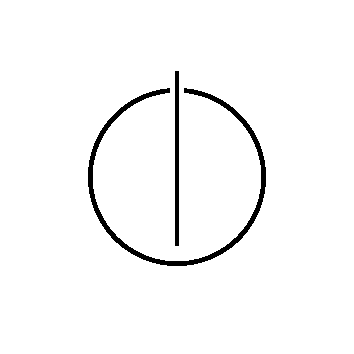
\includegraphics[width=4cm]{styles/informat.png}
  \end{figure}
  
  \end{center}
%	\clearemptydoublepage
	
	%% The titlepage for the CAMP report document.
% Included by MAIN.TEX


%--------------------------------------------------
% The title page
%--------------------------------------------------

% correct BCOR - undo at the end !!!
\def\bcorcor{0.15cm}
\addtolength{\hoffset}{\bcorcor}

\thispagestyle{empty}

 \vspace{10mm}
\begin{center}
	       \oTUM{4cm}
	   
	   \vspace{5mm}     
	   \huge FAKULT{\"A}T F{\"U}R INFORMATIK\\ 
	   \vspace{0.5cm}
	 \large DER TECHNISCHEN UNIVERSIT{\"A}T M{\"U}NCHEN\\
        
	\end{center}
		

\vspace{10mm}
\begin{center}

   {\Large \doctype}

  \vspace{10mm}
  
  {\LARGE \title}\\
  
  
  \vspace{10mm}
  
  
  {\LARGE  \titleGer}\\
  
  
  \vspace{10mm}

    %\hfill
    \begin{tabular}{ll}
	   \Large Author:     & \Large \author \\[2mm]
	   \Large Supervisor:    & \Large Prof. Dr. Hans-Arno Jacobsen \\[2mm]				
	   \Large Advisor:	& \Large M. Sc. Jan Adler\\[2mm]
	   \Large Date:       & \Large August 15, 2016
	 \end{tabular}
	 
	 \vspace{5mm}
	 
	 \begin{figure}[h!]
  \centering
   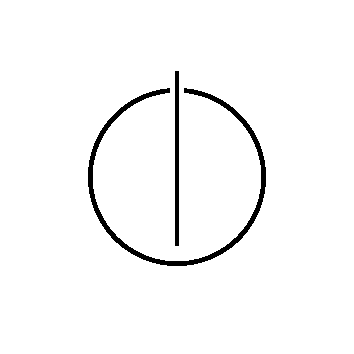
\includegraphics[width=4cm]{styles/informat.png}
  \end{figure}
   

\end{center}

% undo BCOR correction
\addtolength{\hoffset}{\bcorcor}
	
	
%	\input{components/cover_maschmeyer}
	\clearemptydoublepage
	
	% The titlepage for the CAMP report document.
% Included by MAIN.TEX


%--------------------------------------------------
% The title page
%--------------------------------------------------

% correct BCOR - undo at the end !!!
\def\bcorcor{0.15cm}
\addtolength{\hoffset}{\bcorcor}

\thispagestyle{empty}

 \vspace{10mm}
\begin{center}
	       \oTUM{4cm}
	   
	   \vspace{5mm}     
	   \huge FAKULT{\"A}T F{\"U}R INFORMATIK\\ 
	   \vspace{0.5cm}
	 \large DER TECHNISCHEN UNIVERSIT{\"A}T M{\"U}NCHEN\\
        
	\end{center}
		

\vspace{10mm}
\begin{center}

   {\Large \doctype}

  \vspace{10mm}
  
  {\LARGE \title}\\
  
  
  \vspace{10mm}
  
  
  {\LARGE  \titleGer}\\
  
  
  \vspace{10mm}

    %\hfill
    \begin{tabular}{ll}
	   \Large Author:     & \Large \author \\[2mm]
	   \Large Supervisor:    & \Large Prof. Dr. Hans-Arno Jacobsen \\[2mm]				
	   \Large Advisor:	& \Large M. Sc. Jan Adler\\[2mm]
	   \Large Date:       & \Large August 15, 2016
	 \end{tabular}
	 
	 \vspace{5mm}
	 
	 \begin{figure}[h!]
  \centering
   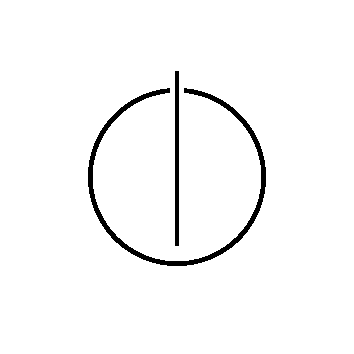
\includegraphics[width=4cm]{styles/informat.png}
  \end{figure}
   

\end{center}

% undo BCOR correction
\addtolength{\hoffset}{\bcorcor}
	
	
	\clearemptydoublepage


\thispagestyle{empty}
\selectlanguage{english}
	\vspace*{0.8\textheight}
	\noindent
	I assure the single handed composition of this master's thesis, only supported by declared resources.
	\newline
	\newline
	\newline
	\noindent
	M{\"u}nchen, August 15th, 2016 \hspace{5cm} \author
\selectlanguage{english}
\newpage
	
	\clearemptydoublepage
\phantomsection
\addcontentsline{toc}{chapter}{Acknowledgements}	


%\chapter*{Acknowledgements}

\vspace*{2cm}

\begin{center}
{\Large \bf Acknowledgments}
\end{center}

\vspace{1cm}

I would first like to thank my advisor Jan Adler for providing me the opportunity to work on an interesting topic and supervising me throughout the research. 
\newline

I thank Prof. Dr. Hans-Arno Jacobsen for providing me an opportunity to write my thesis under the Chair of Distributed Systems. I thank my advisor for providing me valuable feedbacks and suggestion from the start to the end of the thesis.
\newline

I would like to thank my family for giving me the motivation and moral support. I would also like to thank my friends Suvash Sedhain and Niroj Sapkota for their constant support and motivation. And special thanks to my friends for creating a positive environment by cracking jokes and taking off the pressure during coffee breaks.

	
	% Abstract for the TUM report document
% Included by MAIN.TEX


\clearemptydoublepage
\phantomsection
\addcontentsline{toc}{chapter}{Abstract}	





\vspace*{2cm}
\begin{center}
{\Large \bf Abstract}
\end{center}
\vspace{1cm}

% In today's world where billions of people exchange information online, service providers like Facebook, Twitter, Whatsapp store and process tremendous amount of data. Those service providers need distributed scalable storage systems to store and process big volume of data. Even though data are stored in a distributed storage systems, still the huge size of data are bottleneck for performance optimization. Scanning tens of millions rows and few million columns each time are expensive in terms of execution time and processing power. $Materialized$ $Views$ solve this problem by precomputing expensive queries and storing result in a physical table or disk. One of the bottleneck for this approach is constantly maintaining consistency between base table and view table. We propose a $Incremental$ $View$ $Maintenance$ approach to maintain consistency between base table and view table.


In today's world, billions of people exchange information online. Service providers like Facebook, Twitter, Whatsapp store and process tremendous amount of data. Those service providers need distributed scalable storage systems to store and process a big volume of data. Even though data are stored in a distributed storage systems, still the huge size of data can be a bottleneck regarding performance optimization. Scanning tens of millions of rows and few million columns each time are expensive regarding execution time and processing power. $Materialized$ $Views$ solve this problem by pre-computing expensive queries and storing the result in a physical table or disk. One of the bottlenecks for this approach is constantly maintaining consistency between the base table and the view table. In this thesis, we propose a $Incremental$ $View$ $Maintenance$ approach to maintain consistency between the base table and the view table.

	\tableofcontents
  
 % \clearemptydoublepage

\phantomsection
\addcontentsline{toc}{chapter}{Outline of the Thesis}

\begin{center}
	\huge{Outline of the Thesis}
\end{center}




%--------------------------------------------------------------------
\section*{Part I: Introduction and Theory}

\noindent {\scshape Chapter 1: Introduction}  \vspace{1mm}

\noindent  This chapter presents an overview of the thesis and it purpose. Furthermore, it will discuss the sense of life in a very general approach.  \\

\noindent {\scshape Chapter 2: Theory}  \vspace{1mm}

\noindent  No thesis without theory.   \\

%--------------------------------------------------------------------
\section*{Part II: The Real Work}

\noindent {\scshape Chapter 3: Overview}  \vspace{1mm}

\noindent  This chapter presents the requirements for the process.

	\mainmatter
	
	



\chapter{Introduction}
\label{chap:introduction}

At VLDB 2013 Facebooks Vice President of Infrastructure Engineering Jay Parikh stated\cite{parikh:facebook}, that the data warehouse of Facebook is 250 PB in size. Every day, 600 TB of new data are added. The data, which is not older than a day is called $hot\:data$ and it is kept in fast accessible and cached systems. The data, older than a day, is refered to as $cold\:data$. The cold data represents the significantly largest amount of the data volume. It is requested infrequently, but still has to be available to the user. Moreover, the cold data is analyzed, to gain information about the systems or users behaviour. To persist the huge amounts of cold data, $Large\:Scale\:Distributed\:Databases$ are used, e.g. Scuba \cite{barykin:scuba}, Hive, PNUTS\cite{cooper:pnuts}, Dynamo\cite{decandia:dynamo}, Bigtable\cite{chang:bigtable} or HBase \cite{borthakur:facebook}. The distributed nature of these systems make it difficult to retrieve and process data immediately. To analyze the data, it is a common approach, to run queries on multiple nodes in parallel\cite{barykin:scuba}. However, even if the queried data is accessed in-memory and parts of it are cached, querying often involves scanning and recalculating a large amount of base table records. In order to reduce this effort, materialized views have always been a vital option\cite{blakeley:efficiently}\cite{jacobsen:viewmaintenance}\cite{agrawal:asynchronous}. Materialized views can be kept up-to-date by updating them incrementally\cite{gupta:maintaining}.  They guarantee fast access and permanent availability of the aggregated, selected and joined data. Despite their advantages, materialized views are very challenging to the infrastructure, running beneath them. They introduce the problem of view maintenance and complicate the goal of keeping data consistent. In contrast to queries, materialized views are durable. Once a materialized view has become inconsistent, it constantly returns incorrect results. The longer the view is kept, the higher the chances, that data becomes stale. Moreover, there are additional challenges, when integrating materialized views into distributed storage systems. The lack of global synchronization and transactional guarantees can easily lead to corrupt data\cite{jacobsen:viewmaintenance}. We propose a View Maintenance System, that integrates the concept of materialized views with the distributed storage system HBase. We take away the burden of calculating views from the storage servers of HBase and we share the maintenance work among a variable set of $View\:Manager$ components. We show, how we can harness the advantages of materialized views and simultaneously get rid of their negative effects. By doing so, we combine findings in the research field of view maintenance with the advantages of the HBase architecture. We build a View Maintenance System, that is able to safely and efficiently calculate materialized views. 

In Chapter \ref{chap:background}, we analyse the fundamentals of views and view maintenance. In Chapter \ref{chap:relatedwork}, we present research, that is related to this thesis. In Chapter \ref{chap:analysis}, we define the requirements of the View Maintenance System and discuss possible alternatives.  In Chapter \ref{chap:architecture}, we align the architecture of the system and define its functionalities. In Chapter \ref{chap:viewconsistency}, we discuss threats to consistency and apply consistency techniques. In Chapter \ref{chap:loadbalancing}, we show how load balancing can be accomplished in the View Maintenance System. In Chapter \ref{chap:failuredetection}, we take counter measures to component failure. In Chapter \ref{chap:implementation}, we show challenges of the implementation. Finally, we evaluate and interpret the behaviour of the system in Chapter \ref{chap:evaluation}.\\


\chapter{Background}
\label{chap:background}

The first sections of this Chapter explain the fundamentals of Views and View Maintenance. In the following sections technologies are introduced, that are common for todays Large Scale Distributed Databases. The technologies define the infrastructure of the system, that is designed and implemented, later in the thesis. 

\section{Views}
Views are a well-known terminology since the development of relational database systems. Because, there are a lot of queries on the data in a database system, views can be computed. A view makes a database query accessible under a certain name.  This makes life easier for a programmer, because he doesn't need to repeat queries, that are frequently used. Moreover, it reduces complexity, to have a concise name for a query. The view hides the details, for example, if the query statement is very long. Join views for example, span over multiple tables and contain a lot of conditions.
But beyond the practical aspects, a view represents a logical concept.  The result of a query, on the tables of a database system, is nothing more than a table itself. The query selects aggregates or attaches data, but the result set is always a number of data rows, which can be stored like a table. The only difference to a data table is, that the data of the view is derived from already existing data.  A view can be seen as angle of view on the database. In the following, the term $view\:table$ refers to a table representing a view and the term $base\:table$ refers to the data source from which the view is calculated. 


Views are an integral part of relational databases. Nevertheless, views haven't been used a lot by programmers for various reasons.  In $MySQL$ for example, a view is recalculated during every client request. This corresponds to a query, beeing executed for every request. In a small application, with little users, this may be sufficient. However, in the context of larger data sets, repeated tables scans are unfeasible. For that reason, there have been approaches to use $materialized\:views$. Materialized views store the view tables directly on disk, exactly like every other database table. This improves performance significantly, since the view is not recalculated and access to the data is as fast as regular requests. It is only updated, if an insert/update/delete-command has been executed on the data of the base table. Materialized views save a lot of needless recalculations, which is desired, in terms of performance of the database. Unfortunately, the data, that is stored in the materialized view is derived. If a record in the base table changes, then the data in the materialized view is stale. This introduces the problem of $view\:maintenance$. 


\section{View Maintanence}
\label{sec:viewmaintenance}


View maintenance describes the process of updating the view, correspondig to the changes in the base table. Materialized views can be refreshed by recalculating the complete view or by updating those records of the view, which are affected by base table updates. This very efficient way of recomputation is called $incremental\:view\:maintenance$. When performing incremental view maintenance, there are two different options. The first option is the $immediate$ or $synchronous$ maintenance, where the view is updated together with the base table update, in the same transaction. The other option is the $deferred$ or $asynchronous$ maintenance, where the update of the view is shifted to a later point in time. Right, after the base table updates are issued to the database, they are forwarded to another component. The process of forwarding is called $update$ $propagation$. The deferred updates can be applied one by one to the view table. They also can be applied batchwise, in blocks of updates, or on demand, in the moment the client needs the view.  For Large Scale Distributed Databases deferred view maintenance provides some key properties. The storage servers are now able to process more client request per second, because they are not longer bothered with keeping the view up-to-date. Likewise, the view maintenance is decoupled from the storage system. In case, the base table schema is changed and causes the view table updates to fail, the storage servers remain unaffected. But, there are also downsides to deferred view maintenance. Once again, the goal of keeping data consistent is complicated. In the moment, the data is applied to the view, it may be out-dated and stale. Some view types, e.g. the join view, require calls, back to the base table. But in the meantime, the state of the base table may has changed and the delivered data is incorrect. In the thesis, we follow the approach of incremental deferred view maintenance. We aim at using the advantages and simultaneously reduce the negative effects on consistency.


\section{View Types}
\label{sec:viewtypes}


There are different types of views, that can be updated using deferred, incremental view maintenance. These types introduce different challenges to the View Maintenance System. When a base table update is propagated, we distinguish two kinds of view table operations, the local and the global ones. During a local operation, a view record is retrieved from the view. It is updated, and then, put back to the view. During a global operation, the same process happens, but additionally the base table has to be queried, in order to retrieve information, that is not provided by the base table update. Furthermore, the cardinality of the relation between base table and view table records can differ. In some view types, one base table record is mapped to one view record, in other view types, many base table updates are mapped to one view record. Since, we care about view consistency at record level, this is an important aspect.


\subsection{Aggregation}
Aggregation views are all kinds of views, where data of the base table is merged, depending on a particular key. The data can be merged as sum, count, min, max or average of the base table records. Technically, the update procedure remains the same for all cases. By taking the sum for example, the sum over all base records with the same aggregation key is calculated. When using incremental view maintenance, the aggregation key of the base record is looked up in the view table. If the corresponding view record is found, then it is increased or reduced by the delta of the aggregation value. Updates to count and sum views are exclusively local. Only for min and max view, there is a case, where a global operation has to be executed. If in a min view, the minimum of a set of aggregation keys is deleted, the minimum has to be re-evaluated over the whole data set of the base table. The same procedure applies for the deletion of a maximum in a max view. The rest of operations in min and max views is local. The relation between the base table records and the view table records is one-to-many. All base records, containing the same aggregation key, are mapped to the same view record.

\subsection{Selection}
In selection views, base records are just selected according to a condition. Depending on the evaluation of the condition, they are put into the view table or not. Selection views are easy to process considering incremental view maintenance. They only generate local update operations on the view table. Inserts and updates are propagated by inserting or updating the view record. The update of the base table record can render the condition false. Then, the view record has to be deleted. The same happens, in case of the base record, getting deleted. The relation between base records and view records is one-to-one. 

\subsection{Join}
Joins are the most complex case, with regard to incremental view maintenance. Because at least two tables, with two primary keys are involved in a join, a lot of special cases have to be considered. To reduce the complexity, we will only discuss the key-foreign key join view (KF-K). In this type of view, the left table contains a primary key and a foreign key. The foreign key depends on the primary key of the right table. This means, that only foreign keys can be inserted in the left table, that are already existing in the right table. Moreover, primary keys can only be deleted from the right table, if there are no appearances of the key in the left table. This facilitates incremental view maintenance, because lookups have only to be performed on the primary key of the right table. Because, we are using a Key-Value Store, this is a very fast type of lookup. Considering the case, where attributes are joined, that are not primary keys of the join relations, lookups are very expensive. Regarding the right side of the KF-K join view, base records and view records have a one-to-many relation, whereas the left side has a one-to-one relation.




\section{HBase}
\label{sec:hbase}
Large Scale Distributed Databases, as introduced in Chapter \ref{chap:introduction}, are a product of the progress in the IT Industry over the past few years. The user numbers have increased strongly, growing from thousands, to millions of users. Moreover, the exchanged data has become larger, consisting not only of text, but also of photo and video messages. With regard to this use case, traditional, relational database systems are not adequate. They do not provide sufficient performance, to serve the continuously increasing load and store the big amounts of data.

No-SQL data stores are a new kind of database concept, which has gained importance in database technology. One type of No-SQL data store are the Key-Value Stores. The API of a Key-Value Store can be seen like a simple Java Map, which provides the operations put, get and delete. These three operations are sufficient for the client, to manipulate the data of the store. For that reason, the Key-Value Store can be seen as a container of key-value pairs. Specification of data types and relations is avoided. The system has to be flexible, to store any size of data and to split the data into any number of partitions. The parts of the table are distributed over the nodes of the storage system. This guarantees, that large table sizes can be managed. Additionally, the access to a single part of the table is always faster, than the access to the whole table. 

There are also downsides, resulting from the design of the the Key-Value Stores. Data is stored in form of key-value pairs, key and values are written as raw bytes. As stated above, there is no data model defined over the tables of the database. The data of the table is not organized in defined rows and columns, relations between tables are not determined. This enables great flexibility for programmers, but it also means, there are no constraints, ensuring integrity of the data and the relations between the tables. Another disadvantage is the absence of mechanisms, that have been established in traditional databases, e.g. transactions, locking, two-phase commit and globally ordered update logs\cite{jacobsen:viewmaintenance}. Considering the high amounts of updates, that are issued to the Key-Value Store in parallel, it is a big challenge to keep data consistent in a Key-Value Store.

HBase\cite{george:HBase} is one representative of the Key-Value Stores. It is the open source version of Google's Bigtable\cite{chang:bigtable}. HBase has been created with focus on performance, flexibility and fault tolerance. The data model is kept simple, in order to enable spreading and replication of data. The Key-Value Store is designed in a distributed fashion. The architecture allows the definition of tables, that span over multiple storage servers and contain big chunks of data, a scenario, where a classical relational database usually exceeds its limits. At Facebook, HBase is used to build the infrastructure of the message system\cite{borthakur:facebook}. The architecture of HBase consists of a Master and multiple $Region\:Servers$. The task of the Master server is controlling the storage, whereas the Region Servers keep the stored data. If a client wants to put a value to the storage, the request gets routed to the Region Server, that manages the appropriate key range. The Region Servers then answer the request of the client. They can manage one or more key ranges and they can be deployed and removed on the fly. 

In HBase, all data in a table is depending on a primary key. Therefore, the table can be split into key ranges. A key range is called a $Region$. Regions are the logical unit of distribution, so that the table can be spread over many Region Servers. The Region Servers act as a container for the Regions and they can be deployed in any number. A Region Server can hold multiple Regions at a time. Regions can be moved between Region Servers to balance the load of the system or to achieve a smooth distribution of data.  For the purpose of integrating the Region Servers into the View Maintenance System, we have to extend their functionality. We are doing this in a component oriented fashion, so that the additional features can be deployed independently on the Region Server.


The basic Region Server implementation of HBase consists of a $Write\:Ahead\:Log$ and multiple $Region\:Containers$. If a client issues an update, it is routed to the Region Server, hosting the key region of the appropriate key. The client transmits the update to the Region Server. When client updates arrive at the Region Server, they are written to a Write Ahead Log first. In the moment the update is written to the Write Ahead Log, it can be considered as persisted safely. Then, the updates are inserted into a Memstore, to guarentee fast access to the data. After a while, when the memstore exceeds its capacity, the updates are flushed to the actual table file on disk. The table files as well as the Write Ahead Log are written to the Hadoop Distributed File System $HDFS$ and replicated multiple times. If the Region Server crashes and the volatile data in the memstore is lost, the Write Ahead Log is needed for recovery.

HBase is equipped with a $Master$ component. The Master component is not part of the data path. It is just responsible for controlling the Region Servers. By performing  assign and remove commands, it (re-)allocates Regions and ensures a uniformly distributed load. The Master controlls the system state. In case of server crash, the Master collects the abandoned Write Ahead Log and assigns it to a new Region Server. In order to react to system events, the Master keeps an observer registered at Zookeeper. Here, the complete system configuration of HBase is stored. There is only one Master in HBase, making the component a single point of failure. But, there is an option to initialize multiple Masters. If the currently running Master fails, its session node in Zookeper gets destroyed and another Master takes over. 



\section{Hadoop Distributed File Systems}

A Distributed File System is structured like a file system on a single computer. There is a hierarchy of directories and files, originating from a root directory. Every directory and file has a defintion of the users, that are allowed to access it. In a local file system the single unit of storage a physical block on the hard drive. In a Distributed File System it is the whole harddrive of the computer, itself. The network nodes of the Distributed File System from a higher-level hard drive. In contrast to the local file system, this has the following advantages. The storage capacity of a Distributed File System can be extended almost infinitely. If the capacity of the current nodes is exceeding the limit, new nodes with additional capacity can be attached to the cluster. Google used the Distributed File System GFS to realize the storage functionality of Google Mail. The latter is managing Emails of millions of users. This volume of data could never be managed by a local file system, even on a high-performance server. Moreover, the block size in a Distributed File System is significantly higher. It is configured to deal with large chunks of data. Other advantages, that come with Distributed File Systems, are a high degree of availability and fault tolerance. If one node of the Distributed File System crashes, the system is still present to the application, using it. The system is able to recover from node failures, automatically. Usually, there is a replication factor, that can be adjusted in a Distributed File System. A replication factor of three means, that the stored content of a node, is always copied to two other nodes. This way the data is existing three times in the network. When one of the nodes goes down, there are still two copies. The Distributed File System then tries to establish the old replication factor of three as soon as possible.
The enumerated advantages make Distributed File System a good choice for the storage level of Key-Value Stores. Google used the Distributed File System GFS as storage layer for the Bigtable service. Every record, that is put to a table on a storage server of Bigtable, is finally written to a file of GFS. Here the database records and transactions can be protected against server crashes. They are replicated on multiple nodes. The distributed nature of the file system corresponds to the distributed nature of the database. In a typical setup on storage node and one data node of the file system are hosted on the same physical machine. The Hadoop Distributed File System HDFS is for HBase, what GFS is for Bigtable. A Distributed File System that is used to store the physical table files as well as the various log files of HBase. 

 

\section{Zookeeper}
\label{sec:zookeeper}
The coordination service Zookeeper facilitates tasks, that are typical for distributed environments. For example, in a distributed system, there is always the need to store a global configuration. The configuration should be persisted safely and accessible for all components. Zookeeper replicates configuration data to mutiple network nodes. But in contrast to a distributed database Zookeeper is just suited for small chunks of data. To store the configuration information Zookeeper provides a hierarchical data structure of what are called znodes. A znode can have children, that are again znodes. There are two different types of znodes, a persitent or an ephemeral znode. A persistent node lives as long it is not deleted, whereas the the ephermal node is bound to the session of the client, who created it. Ephemeral nodes are a mechanism to control the liveliness of a client. Zookeeper keeps contacting the client with heartbeat messages. If a client doesn't answer anymore, Zookeeper considers it crashed and deletes the ephemeral node.

Zookeeper is an event based system. Observers can be registered to any znodes and to any type of events. If one of the events is triggered, Zookeeper notifies the observer. Possible events are creation, deletion or udpate of a znode or the znode children. Since the tree of znodes is a replicated structure, Zookeeper ensures atomicity and sequential consistency for all client operations. With the aim of achieving high performance, the clients are updated asynchronously. In case a client is notified about an event the registration is lost and the client has to register again.

HBase uses the coordination service Zookeeper\cite{hunt:zookeeper} to store configuration information and to detect failure of single components. It is like HBase a scalable system, so multiple instances can be spawned on different network nodes. This set of nodes is called  $Zookeeper\:ensemble$. All Region Servers have to register at the Zookeeper ensemble. They create an ephermeral node and if one of them fails, Zookeeper notices it. Then a corresponding event is created and the master of HBase is informed. Additionally, Zookeeper is the first contact point for all clients of HBase. Before talking to HBase, the client contacts a random node of the Zookeeper ensemble and is then routed appropriately.



\section{Consistent Hashing}

The advantages of consistent hashing has been examined in \cite{karger:webcaching}. Consistent Hashing is a principle which consistently maps resources to servers or caches. When a resource is delivered to the system, the hashring determines which network node is responsible for it. In contrast to a standard modulo function the consistent hashring allows adding resources, without reassigning most of the resources to other network nodes. 





\chapter{Related Work}
\label{chap:relatedwork}

In this Chapter, we learn about the different approaches, that have been made by researchers to perform view maintenance in materialized views. In the first Section, we describe the origins of view maintenance, in order to extract the basics of this field. In the second Section, more recent work is shown, which builds the starting point of the thesis.

\section{Foundations}

There has been many research in the field of view maintenance in the nineties when relational database systems became important\cite{blakeley:efficiently, gupta:maintaining, zhuge:view, colby:algorithms, wang:efficient}. This research has layed the foundations to caclulate materialized views safely and efficiently. In \cite{blakeley:efficiently} an algorithm is developed, that reduces the number of base table queries, during the update of a join view. In \cite{zhuge:view} the ECA algorithm is developed, which prevents update anomalies. When base table updates of join views are processed, queries have to be sent to the data sources, to evaluate the matching rows. While the matching rows are evaluated, further updates can be processed. They can have an effect on the result of the queries, called error terms. The ECA algorithm compensates the error terms by subtracting them from the results. In \cite{colby:algorithms} the basics of deferred view maintenance are layed. The possiblity of differential tables, that keep a precomputed delta of the view table, are researched. Multiple algorithms are suggested to perform deferred view maintenance. Incremental, deferred view maintenance can save a lot of computing time but in return is a big challange towards consistency. Lots of efforts have been made to prevent update anomalies when using incremental view maintenance\cite{gupta:maintaining, zhuge:view, salem:how}. However, the concepts, that are researched in the discussed papers, were designed to meet the requirements of that time. The data sets were centralized and of manageable size. Relational database systems used a database management system to provide access to the data and simultaneously ensure transactional consistency. Usually, the databases were standalone and the update load on the system relatively low. We are still able to use theoretical concepts of that time, but especially the architecture of the systems has changed to what is described in Chapter \ref{chap:introduction}.

Particularly, in the context of datawarehouses view maintenance has been researched extensively. In papers\cite{wang:efficient}, \cite{agrawal:efficient} and \cite{zhuge:strobe} the first approaches are developed to integrate incremental, deferred view maintenance in the context of multiple data sources. In \cite{zhuge:strobe} the strobe algorithm is created. It is a refinement of the ECA algorithm in \cite{zhuge:view} and deals with update anomalies, that occur, when multiple base table updates of a join view arrive at different data sources. In \cite{agrawal:efficient} the sweep algorithm is defined. The algorithm is evaluated with the help of a consistency model. The consistency levels of the model are convergence, strong consistency and complete consistency. A consistency model is introduced to the view maintenance context, for the first time. The sweep algorithm is defined to guarantee complete consistency. Like the ECA and the strobe algorithm, the sweep algorithm compensates error terms of interfering updates, as explained above. But the sweep algorithm does compensation more efficiently. Instead of sending compensation queries to the data sources, it evaluates and compensates the error terms locally at the data warehouse. This is called on-line error correction. In \cite{wang:efficient} the consistency model of \cite{agrawal:efficient} is apdopted and extended with the level of weak consistency. An algorithm is developed that improves the performance of sweep. Thoughts arise, that complete consistency is not needed in most contexts. Therefore it can be dropped in order to gain computation speed. The research on data warehouses is closer to the architecture of Large Scale Distributed Databases than the context above. But the data warehouse is still a central component, where the flow of base table updates is joined. Here transactions can be serialialized in order to build a global order. In the context of HBase, the architecture is completeley distributed. The base table as well as the view tables are partitioned and spreaded over the network.


There have been used versioning and timestamp based approaches to defer view maintenance and ensure data consistency, simultaneously\cite{salem:how, zhou:lazy}. In \cite{zhou:lazy} a SQL version store is used to categorize every update. The update operations receive a transaction number, as well as a statement number within the transaction. These sequence numbers increase monotonically and build an absolute ordering of updates on a global level. Now, the view maintenance can be shifted to any point in time. When executing the view maintenance, the information needed in order to process the base table updates, is taken from the version store. This means, the database can be queried in exaclty the state, it has been in, when the base table update was applied to it. Futher research is conducted on what is called scheduling of view maintenance tasks in \cite{zhou:lazy}. View maintenance tasks consist of blocks of updates, that are applied to the view. The tasks are processed at points in time, where the update load on the system is low. This way the server is relieved in times of heavy update load. The view maintenance task are always applied in right order. As an optimization they can be combined to bigger tasks in order to reduce overhead during view maintenance. There are approaches in \cite{zhou:lazy}, but in the distributed database HBase we cannot rely on time synchronization. HBase provides features of row versioning, but the time on each Region Server might be different. Especially, if Region Servers are distributed geographically, a global notion of time cannot be achieved. Furthermore the authors in \cite{zhou:lazy} assume, that view maintenance is processed, when the system has free cycles. In many of todays large scale Internet platforms, the update load is constantly high. In such an enviroment we need a way to completely relieve the stroage server from the view maintenance.





\section{Recent Research}

The research in  \cite{chen:multiversion} solves consistency problems in materialized views, that are calculated out of losely coupled independent data sources. A data source is a similar term, for what we call a part of the base table. By doing so, in \cite{chen:multiversion} the problem of view maintenance, as described in Section \ref{sec:viewmaintenance}, is extended. The paper also covers the problem statements of view synchronization and view adpation. These both problem definitions deal with schema changes in the base table, which have to be reflected in the view table, dynamically. In contrast to \cite{jacobsen:viewmaintenance} and \cite{agrawal:asynchronous},  \cite{chen:multiversion} is focused on serializing transactions on a global level. Therefore, additional information are stored at the data sources, which apply a logical timestamp to every update records. Moreover, meta information is stored, in order to react to schema changes, properly. While updating the view, a vector containing the different timestamps from the data sources, is maintained. This vector specifies the state a data source has been in, when propagating the update. It can be used to clearly distinguish the order of updates at the view table. Aiming at completely correct ordering of transactions, there is no notion of consistency levels. In \cite{jacobsen:viewmaintenance} and \cite{agrawal:asynchronous} consistency is bound to a certain cost. The higher the consistency level, the higher the cost. The architecture in \cite{chen:multiversion} is a classical data warehouse structure. There are multiple, loosly coupled data sources and one data warehouse. This facilitates View Maintenance to a great extent because the view table is always accessed by the same process. In \cite{jacobsen:viewmaintenance} view tables are distributed and access to them is concurrently. There is no central point in the system, where transactions could be serialized. The latter enviroment, is what we strive for, in the thesis. Furthermore, we want to avoid storing additional data at the data sources like in \cite{chen:multiversion}. We just want to use the build-in mechanisms of HBase in order to achieve the goal of consitent data. 


The paper \cite{jacobsen:viewmaintenance}  brings View Maintenance to Large Scale Distributed Databases. The paper starts with a more general definition of the distributed architecture, that is named Web Data Platform. The term Web Data Platform is similar to what we call View Maintenance System. In the context of Web Data Platforms, the term View Manager, as an independent component for updating views, is defined for the first time. Updates, that are issued to the storage servers are propagated to the View Managers.  View Managers relieve the storage servers, by taking over the work of recalculating the View Tables. Like the storage servers, View Managers are distributed. They can be deployed at any time in the places, they are needed. In \cite{jacobsen:viewmaintenance} data consistency is identified as the most challenging problem during the process of propagating the updates and calculating the views. To measure the consistency, a consistency model is introduced and different levels of consistency are defined. Afterwards, different scenarios are discussed, that lead to inconsistent data. In order to prevent those scenarios, various techniques are applied, e.g. Signatures, Test-And-Set-Methods or Flow Control. The techniques are combined to a set of algorithms, which run on the View Managers. There are different algorithms for different view types, e.g. sum/count, min/max, selection, join. Finally, the researched algorithms are applied to the consistency model. The consistency level, that can be guaranteed, is proven on a theoretical base. \cite{jacobsen:viewmaintenance} builds the theoretical foundations of the thesis. We adopt the context and some of the main ideas of the paper, e.g. the View Managers. But whereas \cite{jacobsen:viewmaintenance} is focused on theoretical aspects of view maintenance, this thesis is concerned with the realization of a View Maintenance System.  We integrate the theoretical approach into an existing Key-Value Storage. Furthermore, we show how View Maintenance can be done in a dynamic and scalable way. Extending the theoretical reasearch, we enhance the consistency, by further developing the ideas in \cite{jacobsen:viewmaintenance}.

Another paper, that also researches View Maintenance in the context of Large Scale Distributed Databases is \cite{agrawal:asynchronous}.  In the paper the terms Remote View Table and Local View Table are introduced. Remote View Tables stand for view tables, that are kept in a separate table on different storage server. Local View Tables on the contrary are kept on the same storage server as the base table. They try to use the advantage of proximity. In \cite{agrawal:asynchronous} the mechanisms of incremental, deffered View Maintenance are applied to the architecture of Yahoo's PNUTS\cite{cooper:pnuts}. By using PNUTS, already existing mechanisms, e.g. failure recovery, performance optimization are extended to the View Maintenance System. There is a component, that is equivalent to the View Manager, called View Maintainer. In contrast to the View Manager, the View Maintainer is always bound to the storage server, where the base table updates originate. The view types, that are supported in \cite{cooper:pnuts} are Equi-Joins, Selection views and Group-by-aggregation views.
Like in \cite{jacobsen:viewmaintenance} timeliness can only be guaranteed for a single record. Consistency in \cite{agrawal:asynchronous} is also researched with the help of a consistency model. However, the consistency model differs from the model in \cite{jacobsen:viewmaintenance}. It is strongly bound to the PNUTS architecture. The statements are not as general valid as in\cite{jacobsen:viewmaintenance}. Calls to a view record may involve callbacks to the base table. There are thoughts on making the view storage fault tolerant. View tables are replicated by the underlying PNUTS architecture.  


\chapter{Analysis}
\label{chap:analysis}

In this Chapter, we analyze the possiblites of building a system, that is able to perform proper View Maintenance in distributed storage system. In the first Section, we define the requirements, that are made to the system. In the second Section, we discuss alternatives of calculating view tables in HBase. We judge the alternatives by their ability to fullfill the requirements.


\section{Requirements}

The requirements are defined as follows. The distributed Key-Value Store HBase has to be used to store the base table and the corresponding view tables. The view tables should be calculated from the base table by using incremental, deferred view maintenance as explained in Section \ref{sec:viewmaintenance}. By doing so consistency of data should be ensured to a reasonable degree, which has to be defined. Mechanisms have to be established, that prevent updates from being applied twice, not in order or not at all to a view table.  

The distributed Key-Value Store HBase offers performance, scalability and recovery mechanisms in the presence of failure. We want to inherit these desirable properties to view maintenance. A View Maintenance System for materialized views should be able to handle changing sizes of workload. There should be a component of scalibility, that can propagate view updates and that can be dynamically added, as the number of updates grows. Additionally, a View Maintenance System should have the ability to shift workloads between the components, to achieve an efficient usage of resources. Different data sets may generate different update distributions and the View Maintenance System should then react accordingly.

When operating large scale internet platforms, we can state that failure is not the exception but the norm. Especially, in the case of horizontal partitioning, commodity hardware is likely to fail\cite{chang:bigtable}. Therefore we want to equip our view maintenance system with recovery mechanims. The system should be able to detect crashed View Managers. It should automatically recover from the crash scenario. Lost updates should be retransmitted and the update flow should be redirected to other working View Managers.


\section{Alternatives}
\label{sec:alternatives}

The naive approach would be, to execute a scan over the whole base table. This is not very efficient. The requests take a very long time because the client scans every Region Server, sequentially until the whole base table has been traversed. The work of scanning the base table, can be parallelized. Therefore, a concept  of HBase called Endpoint Coprocessor is used. It is a piece of code, that is sent to every Region Server and executed there. This way a sum view can be calculated, for example. The piece of code, that the client sends, scans the rows and summarizes the values of a certain aggregation key on every Region Server. Then, the Region Server sends back the intermediate results. The client aggregates the intermediate results of all Region Servers, to retrieve the final result. This approach significantly improves the request times for the client. But with an increasing number of client requests, the network gets flooded by messages between clients and Region Servers. Because the Region Server has to send back a list of aggregation values, the messages can grow very large. For that reason, this approach is fine for small environments, but not for Large Scale Distributed Databases.

Another possibility, that can be used in HBase are update hooks. Here, the program code is deployed directly on the Region Server. When issuing a put operation, the hook is called before the operation is executed and the parameter of the operation are handed over. The Region Server now requests and updates the view record autonomously by using the HBase client API. This is a more efficient solution, since we refresh the view locally and recordwise. The view is materialized and the system can serve a growing number of view requests. As a downside of this approach, we cannot change the view definition. It is hard coded into the program, that we deploy on the Region Server. Moreover, the burden of updating the view is located at the Region Servers. If the cluster of Region Servers is confronted with heavy loads, then the performance of the system will begin to slow down. The Region Servers will have to serve client requests and query the view table at the same time. 

For that reason, we take the approach of using View Mangers, as it is described in \cite{jacobsen:viewmaintenance}. The updates are propagated from the Region Server to the View Managers. The propagation is done asynchronously by reading from the Region Server log. Using the HBase client API is avoided, such that the Region Servers can focus on serving the client requests. 


\chapter{Architecture}
\label{chap:architecture}

In this Chapter, we give an overview of the system, that we intend to build on top of the HBase data store.  Then, we introduce all components of the architecture in detail. Subsequently, we show how the components interact, to create higher level processes. Finally, we show the operating mode of the system, with a little example, illustrating the path of an update, traveling through the system.



\section{System Overview}
\begin{figure}[h!]
  
  \centering
    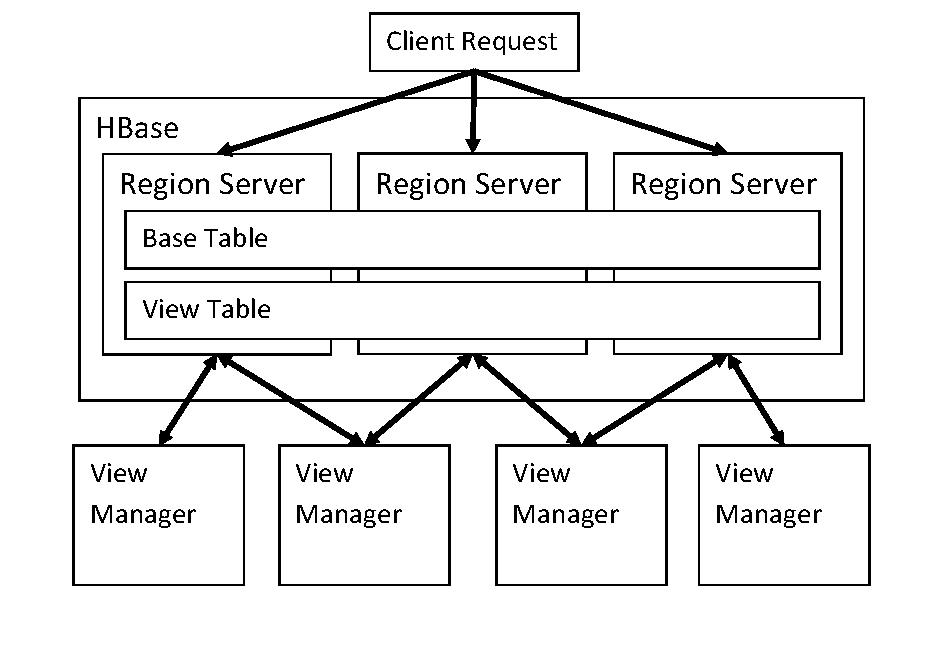
\includegraphics[width=\linewidth]{SystemOverview2}
    \caption{System overview}
    \label{fig:systemoverview}
\end{figure}




In Figure \ref{fig:systemoverview}, the overview of the complete system is shown. On top of the architecture reside the clients, issuing updates to the base table. Below the client, the Key-Value Store HBase is located. On the one hand, we use HBase simply as a data storage. We issue updates and send queries to the client interface. We retrieve base table data and create view tables out of it. On the other hand, we adopt  architectural patterns of HBase, to build up a $View\:Maintenance\:System$. Similar, to the Region Servers of HBase, we define a unit of scalability, called $View\:Manager$. The View Maintenance System is, like HBase, controlled by a Master component, which does not lay on the data path. Additionally, we use the distributed coordination service Zookeeper and we also write to the underlying HDFS, to persist changes.

We are using incremental, deferred view maintenance. Therefore, the updates on the basetable are not processed at the Region Servers. Instead, they are propagated to the View Managers. The View Managers remove the burden of updating the view from the Region Servers. Once the View Manager has been assigned to a Region Server, the Region Server streams all arriving updates to the View Manager. Subsequently, the View Manager processes the updates. It retrieves the corresponding view record from the view table. Then, it calculates the new view record by adding the delta of the base table update to the view record. Finally, it writes back the result to the view table.

A View Manager is the unit of scalability in the View Maintenance System. If a Region Server is overloaded, additional View Managers can be assigned to it. The relationsship between Region Servers and View Managers is a one-to-many relationsship. Multiple View Managers can be attached to a Region Server. Then, the stream of updates is divided and the updates are processed concurrently. To allow scalability, independent of the scenario, View Managers should be exchangable at any time. This means, a View Manager is always able to process any base table operation on any view table at any time. If a View Manager crashes, another View Manager can immediately take over. If a View Manager is reassigned, it moves from on Region Server to the next and continues working without interception.

As mentioned above, due to its design goals, HBase is not equipped with a powerful query language. View managers are able to bring back the expressivness of views to the system, without hurting the performance of HBase. Following types of views can be created: count, sum, min, max, join and selection. We are using a primitive query language, e.g a sum view is defined as $basetable(viewtable$ $sum,$ $aggregationKey,$ $aggregationValue)$. 
The View Managers are doing their view maintenance work in parallel. For that reason, a large number of views can be defined and kept up-to-date simultaneously. In most data warehouse enviroments, the data sources are distributed and the warehouse is centralized\cite{chen:multiversion}. Our approach is capable of splitting the base table, as well as the view tables into multiple Regions and distribute them over the Region Servers.\\   

\section{System Components}
\label{sec:systemcomponents}

In the following, we explain the components, that we developed, in order to build up a View Maintenance System.  We start with the master, that is controlling the system. Then, we go on describing the extensions we made to the HBase Region Server. Finally, we introduce the View Manager, which represents the core component of the View Maintenance System \\



\subsection{VM Master}
HBase uses a Master component to control the storage system. We want to use a similar mechanism, to control the View Maintenance System. Because, we don't want to interfere with the HBase Master, we create our own Master component, called $VM\:Master$. A presentation of the VM Masters architecture is shown in Figure \ref{fig:master}. The View Managers in the system are assigned to Region Servers dynamically. The VM Master determines, which View Manager is assigned to which Region Server. Moreover, the VM Master takes care of the systems running condition. In case of a View Manager crashing, the VM Master takes measures, to guarantee an errorless recovery. It continously monitors the systems state and is able to control the components remotely. The VM Master consists of four subcomponents: the $Event\:Processor$, the $Load\:Balancer$, the $Recovery\:Manager$ and the $Component\:Controller$. 

The Event Processor observes the events occuring in the system. If any system component is added, removed or crashes, the Event Processor is informed. Then, it creates an event and passes it either to the Load Balancer or to the Recovery Manager. All standard operating procedures, like adding and removing components, are forwarded to the Load Balancer, while a crash event is handed over to the Recovery Manager. 

The Load Balancer tries to balance the systems load by assigning View Managers to the Region Servers. The load balancer is always called, when a component is added, removed or has crashed. Likewise, it is able to perform a temporary load balancing and shift the hardly loaded or idle View Managers from one Region Server to another. To calculate the load plan, the Load Balancer needs to be informed about the utilization of the components. Therefore, the number of updates, that are currently pipelined, is aggregated in a treewise fashion from the View Manager to the Region Server to the VM Master. The Load Balancer holds a reference to the Component Controller to execute its load plan.

The Component Controller represents the VM Masters interface to control the entire View Maintenance System. It contacts the compenents and uses a message protocol to transmit commands. The Component Controler is used, to realize the caclulated load balancing actions. It also receives confirm messages from the components, to verify, that a given instruction has been executed by a component. This is vital, to keep a consistent system state.\\

The Recovery Manager is informed in case one of the components crashes. When a View Manager crashes, the Recovery Manager performs an action to find out the last processed updates. It then, informs the Region Server, to replay and reassign the updates, that might have been lost during the crash of the View Manager.



\begin{figure}[h!]
  
  \centering
    \includegraphics[width=\linewidth]{RegionServer}
    \caption{extended Region Server}
    \label{fig:regionserver}
\end{figure}

\subsection{VM Region Server}
\label{subsec:vmregionserver}
The Region Server of the View Maintenance System extends the architecture of a Region Server of HBase. Therefore, we call it $VM\:Region\:Server$. The components, which are added for view maintenance purposes, can be seen in Figure \ref{fig:regionserver}: the $WAL\:Reader$, the $Update\:Assigner$ and the $Update\:Distributor$. The updates are passing these components sequentially, in exact that order.  The VM Region Server is then, able to, not only persist the update operations of the clients, but also forward the updates to a large number of registered View Managers. 
 
The WAL Reader compenent is able, to connect to the file system HDFS. If updates are inserted to the Write Ahead Log, the WAL Reader starts reading them. By doing so, the updates are propagated completely asynchronous. The updates are listed in the Write Ahead Log in strict FIFO order and they are tagged, with a unique, sequential number. Later, this helps us to globally identify the updates. The WAL Reader acts like a pointer to the Write Ahead Log of the HBase Region Server. It constantly polls the log folder of the Region Server. If it has found new update entries, it points to the line in the log file and starts reading the updates. If problems occur during update propagation, the WAL Reader is able to jump back to a previous line of the Write Ahead Log and to read the updates several times. This procedure is called $replaying$ the Write Ahead Log. After the WAL reader has extracted the updates, it forwards them to the Update Assigner.

The Update Assigner is responsible for assigning the updates to the View Managers. It uses a consistent hash ring.  Every View Manager, which registers at the Region Server, is inserted into the hash ring. A hash value is calculated from the View Managers system ID. This hash value is then put to a treemap, implementing the hash ring. If a View Manager leaves, it is deleted from the hashring by removing its entry in the treemap. To assign a key to a View Manager the Update Assigner calculates a hash value out of the key of the base table update. Then, the View Manager, laying closest to the key on the hashring clockwise, is determined. If the assignment has been carried out, the Update Assigner delivers the update to the Update Distributor. By using consistent hashing, only a small amount of keys has to be remapped, in case a new View Manager is added or removed. Consistent hashing is a key aspect, when establishing flow control and providing consistency guarantees in the View Maintenance System.

The Update Distributor creates an own queue for every View Manager. Depending on the assignment, the update is put to the corresponding queue. From there, the updates are sent to the View Managers in FIFO order. To speed up update distribution, the update distributor runs every queue separately. It doesn't wait for acknowledgements, but pushes the updates to the View Managers without delay.
 
Finally, there is a $RS\:Controller$ component, which is not involved in the update processing. Instead, it is conducting all internal components. When the Region Server starts up, the controller initializes every component. Moreover, it is the interface through which other components can talk to the Region Server. The VM Master for example, uses the RS Controller to remotely controll the functions of the Region Server.\\ 

\subsection{View Manager}

Like stated above, the View Manager is the component of scalibility. A detailed picture of its architecture is depicted in Figure \ref{fig:viewmanager}. The View Manager is able to process view updates at record level. The subcomponents, that are handling the update processing are the $Pre\:Processor$ and the $Processor$.

The Pre Processor resolves the view tables, that are mapped to a base table update. This procedure can change the number of processed updates dramatically, e.g. if a lot of views are assinged to one base table. For that reason, the Pre Processor measures the current load of the View Manager. The information about the load state is then send back to the Region Servers periodically.

The Processor performs the actual work of computing the view deltas. It can retrieve view records from the view tables. Subsequently, the Processor queries the base table. This is an optional step, since most of the updates are local. For example, all update operations on a sum view are local, because only the difference of the client update has to be added or subtracted from the view table record. A global operation would be the deletion of a current minium in a in min view. Then, the whole base table had to be queried to find a new minimum. 

As the most important step, the Processor calculates the new value of the view record and updates the view. Because the view can also be a distributed dataset the Processor may contact multiple Region Servers. Additionally the Processor maintains a $Commit\:Log$. There, it puts the base table updates, indicating, that they have already been processed. The Commit Log is like the Write Ahead Log written to the HDFS.

\section{System Operations}
\label{sec:systemoperations}

In order to control the View Maintenance System, we have to define the possible system operations. The system operations should be executed atomically and leave our system in a consistent state. System operations can be either triggered by system events or by the VM Master to transform the systems state. The VM Master keeps a model of the system state stored in the systems configuration. This model contains a list of View Managers, Region Servers and a map of assignments, showing the assignment of View Managers to Region Servers.\\

\noindent  
\textbf{Add View Manager -- }Adding describes the process of adding a new View Manager resource to the View Maintenance System. When a View Manager is added to the system, it primarily contacts the Zookeeper ensemble. To register at the View Maintenance System it creates a session node in the View Manager branch of Zookeeper. The session nodes are called ephemeral nodes in Zookeeper. The master component keeps an observer registered to the View Manager branch and is informed as soon as a new node is created. When the master notices the creation of a new View Manager it updates the system configuration and immediately assigns the View Manager to the most loaded Region Server. A visualisation of the process can be seen in Figure \ref{fig:addviewmanager}.\\

\noindent  
\textbf{Remove Manager -- }Removing describes the process of deleting a View Manager resource from the system. A remove operation can either be initiated by the master, sending a remove command or by the viewmanager itself. However, the View Manager cannot be removed instantaneously. It might be, that the queues of the View Manager are full of updates. Then, the View Manager needs some time, to finish its work. Nevertheless, incoming updates have to be stopped from beeing assigned to that particular View Manager. For that reason, the View Manager sends a withdraw command to the Region Server. In the last step, the View Manager waits until the updates have been processed. At that point in time, the deletion of the View Manager is still not acknowleged at the VM Master. If the View Manager crashes, while processing the last updates, the VM Master is notified and replays the updates. Only, if the View Manager has processed the last updates safely and confirmed the removing the VM Master accepts the disappearance of the View Managers session node.\\ 

\noindent  
\textbf{Assign View Manager -- }Assigning a View Manager describes the procedure of attaching it to a Region Server. In contrast to the add operation, the View Manager is already part of the system. It is registered at Zookeeper and the VM Master knows about its existence. The master then initiates the procedure by sending an assignment command, including the targeted Region Server as a parameter, to the View Manager. From there on, the View Manager handles the assignment by itself. It sends a $request$  $assign$ message to the Region Server. The Region Server registers the View Manager by performing several initialization steps. It adds the View Manager to its hash ring and creates a queue, where the assigned updates are stored. The Region Server then runs a thread, that contacts the View Manager and starts sending the updates from the queue. To complete the process the Region Server sends an acknowledgement, confirming, that the View Manager has been added. The View Managers forwards the acknowledgement to the VM Master, indicating that the procedure has been finished. We intentionally exlude the VM Master from the  assignment procedure to not overburden it with communication tasks. Especially, when scaling to several hundreds of nodes this aspect is critical. A visualisation of the process can be seen in Figure \ref{fig:assignviewmanager}\\
 
\noindent  
\textbf{Withdraw View Manager -- }The withdrawing operation of the View Manager is contrary to the assign operation. It takes away the View Manager from the Region Server. In contrast to the remove operation, the View Manager remains in the system and can then be used as a free resource. The withdraw operation is initiated by the VM Master, sending a withdraw command to the View Manager. The View Manager then forwards the command to the Region Server. The Region Server performs the same steps as for the assignment, but in the opposite order. It takes away the View Manager from the hash ring such that no more updates can be assigned. Then, after the last updates are transmitted it stops the sending thread and removes the update queue. To complete the process it sends a confimation message to the View Manager. The View Manager informs the VM Master, which updates the systems configuration. A visualisation of the process can be found in Figure \ref{fig:withdrawviewmanager}\\

\noindent  
\textbf{Reassign View Manager -- }A reassign operation is used to move a Region Server from one Region Server to another. It is frequently performed during load balancing. The operation is initiated by the master, sending a reassign command to the view manger. The View Manager simply cascades the operations withdraw and assign. When it receives the assigment confirmation of the target Region Server it sends an acknowledgement to the master. A visualisation of the process can be found in Figure \ref{fig:reassignviewmanager}\\

%\end{itemize} 

We designed the system operations according to the ACID principles. The system operations are always commited by the VM Master, updating the systems configuration accordingly. This is supporting atomicity, because, if a system operation somehow fails, then the system configuration is not updated. Only, a completely successful operation is recorded by the master. Isolation of system operations is quaranteed by the VM Masters subcomponent Component Controller. The Component Controller executes the commands, which are performed as part of the system operations, one after the other. There is a property, specifying a fixed number of retries, in case a component is not answering. A View Manager changes its state from "running" to "assigning", when receiving an assign command. In case, a second command is sent by the master, while the View Manager is executing the first command, then the former is beeing denied. However, the system operations are not perfectly consistent. A system operation, like the assignment of a View Manager, may be executed successfully and then, the final message to inform the VM Master gets lost. The system state is not be reflected in the systems configuration then. But regarding the case, we can also conclude that the systems operability will not be hurt. The Region Server forwards updates to the View Manager, which processes the updates typically. As soon as the VM Master performs the next load balancing, it notices an idle View Manager and reassigns it, reasonably. The systems configuration is persisted safely by storing it to the Zookeeper, guaranteeing durability of the system operations. 

\section{Update path}
Exemplarily, we show how an update travels through the system. Consider a base table relation $R(\underline{K},X,Y)$. Two views $S_1(\underline{X},Y)$ and $S_2(\underline{X},Y)$ are defined over the base table. The base table is stored on two Region Servers $rs_1$ and $rs_2$. Two View Managers $vm_1$ and $vm_2$  are assigned to the Region Server $rs1$, one View Manager $vm_3$ is assigned to $rs_2$. In order to perform the insert operation $i_1(R(k1,x1,50))$ to the base table, the client contacts the Zookeeper ensemble. From there, the client is routed to Region Server $rs_1$, because $rs_1$ is serving the key region key $k_1$ belongs to. The client sends a put operation, containing $i1$ to the HBase client interface. The Region Server accepts the update and stores it to its Write Ahead Log. Now HBase proceeds by putting the update to its Memstore and, if the Memstore is full, flushing it to disk. Anyway, the Wal Reader component, which is part of the Region Server extension, collects the update $i_1(R(k1,x1,50))$ from the Write Ahead Log. It passes the update to the Update Assigner.  The update assigner caluclates a hash value $h(k_1)$ out the key $k_1$. Then, it uses the hash ring and determines, that View Manager $vm_1$ is responsible for $k_1$. The Update Assigner calls the Update Distributor, handing over the name of $vm_1$ and the update $i_1$. The Update Distributor puts $i_1$ to the queue of $vm_1$. From here, it is transferred to $vm_1$.\\
$vm_1$ preprocesses update $i_1$. It identifies the base relation $R$ and resolves view $S1$ and $S_1$. The Pre Processor generates two updates out of $i_1$, namely $i_{1,S1}$ and $i_{1,S2}$. Then, it passes the two updates to the Processor component. The Processor  retrieves the view records $S_1(x1, 20)$ and  $S_2(x1, 50)$. It incrementally adds $i_{1,S1}$ and $i_{1,S2}$ to both view records, resulting in $S_1(x1, 70)$ and  $S_2(x1, 100)$. In the last step, $i_{1,S1}$ and $i_{1,S2}$ are written to the Commit Log of $vm_1$, indicating that the work for these updates has already been performed. A visualisation of the process can be seen in Figure \ref{fig:updatepath}  



\chapter{View Consistency}
\label{chap:viewconsistency}
In this Chapter, we discuss how consistency can be established with regard to the systems architecture. In order to measure and compare consistency, we define a consistency model and the corresponding consistency levels. In the main Section, we classify scenarios, that are challenging to the consistency. For every scenario, we make a little example and propose a solution. 


\section{Consistency model}
\label{sec:consistencymodel}

The consistency model formalizes the process of view maintenance and introduces the different levels of consistency. Because there has already been research on consistency in view maintenance\cite{zhuge:strobe, jacobsen:viewmaintenance} we adopt the consistency model of Jacobsen and apply it to our architecture.
In the model $B$ represents our base table, whereas $V$ represents our view table. Both tables change as we are starting to issue updates. Therefore we use the notion $B_i$ and $V_j$ to specify the state of the respective table. Because we are interested in view consistency at record level we write $B_i(r)$ and $V_i(r)$ to indicate a state of a single record of the table. The initial baste table state is denoted with $B_0$. If we now store some updates to the base table, the records in the table change and we enter an immediate state $B_i$ with $B_0 < B_i < B_f$. Finally we enter $B_f$, which is the state when all updates have been applied. Simultaneously the View Maintenance System propagates the updates and applies them to the view. Similarily, the view starts with state $V_0$ and ends up with $V_f$. The view does not necessarily represent the correct derivation of the base table. Therefore we use a function $view(B_i)$ to indicate how the view table should look like. Then we can compare the current condition of the view to the desired condition. To compare base or view table states to each other we write $B_i \leq B_j$. This means for every record $r$ the following holds true: The version of record $r$ in $B_i$ is smaller or equal than the version of record $r$ in $B_j$. By version we are refering to the $timeline$ of a record. Every time we update a record we produce a new version of it. The timeline of a record plays an important role. In a ditributed data store, we assume that servers are not perfectly synchronized in time. For that reason we cannot make any statements about the the global order, in which the updates are happening. But since an update of a single row always occurs at the same server we can rely on the order of updates to this row. In the following we call this property $timeliness$. 


\subsection{Levels of Consistency}
To measure and compare consistency within the View Maintenance System, we introduce consistency levels.  In order to describe the levels we use the terms of the consistency model. The consistency levels build on top of each other, meaning every level requires the preceding level to be fulfilled\\
\noindent  
\emph{Convergence -- }Convergence describe the simpest level of consistency, where the view table has been calculated correctly. The end states of the base table $B_f$ and the view table $V_f$ correspond to each other, denoted by: $V_f(r) = (View(B_f))(r)$\\\\
\emph{Weak consistency -- }We achieve convergence. Moreover every view state that is generated through the view maintenance process correspondes to a base state. However, not every base state has to be reflected. For each intermediate state of the view table the following holds true: $V_j(r) = (View(B_i))(r)$\\\\
\emph{Strong consistency -- }We achieve weak consistency. Moreover the intermediate view table states are ordered corresponding to the base table states. This means if $B_{i1} \leq  B_{i2}$ then $V_{j1} \leq V_{j2}$\\\\
\emph{Complete consistency -- }We achieve strong consistency. Moreover every base table state $B_i$ is reflected by a corresponding view table state $V_j$. In most cases it is enough for the client to retrieve a consistent view state. It is not necessary that every possible base state is reflected in the view.

\section{Threats to consistency}
\label{sec:threatstoconsistency}
Because we cannot prove cosistency at once, we group the threats to consistency into different classes. First we describe the nature of the problem and illustrate it with an example. Then, we develop a solution to avert the threat. We do so by establishing appropriate mechanisms in HBase and the View Maintenance System. In Figure \ref{fig:co_consistencyproblems}, a time flow diagram of the threats is depicted.\\
 
 
\subsection{Non idempotent updates} 
\label{subsec:nonidempotentupdates}
In the View Maintenance System, updates are sent over the underlying network several times. Since we can not always rely on perfect transmisson, messages have a chance of beeing duplicated. Moreover, the process of recovering from View Manager crashes, forces us to replay the Write Ahead Log of the Region Server. In both cases, duplicated updates are send repeatedly to a View Manager. This can have severe consequences on consistency, because the same update is applied several times. In a sum view for example, convergence can be violated, as the following example shows.\\
 
\noindent 
\emph{Example -- }We define a base table $R(\underline{K},X,Y)$ and view table $D(\underline{X},S)$. The view is defined as
\begin{verbatim}
	SELECT SUM(Y) FROM R GROUP BY X
\end{verbatim}
The initial table states are $B_0\{R(k1,x1,50)\}$ and $V_0\{D(x1,50)\}$. There is one insert $i_1(R(k2,$ $x1,100))$. Because of transmission problems or recovery actions insert $i_1$ gets duplicated and is transferred to View Manager $VM_1$ twice. $VM_1$ updates the view record twice, leading to a final view table state $V_f\{(x1,250)\}$ where it should be $V_f\{(x1,150)\}$. A diagram of the example is shown in Figure \ref{fig:co_nonidempotentviewupdates}.

\noindent  
\emph{Solution -- }To solve the problem of idempotent view updates, we have to use signatures of view records. Signatures are a suggestion in \cite{jacobsen:viewmaintenance}. The signature reflects the state of a view record. Every time a base table update is applied to the view record, the signature is recalulated by appending the id of the base table update. If adding another base table update yields the same signature, the udpate has already been applied.


\begin{figure}[h!]
  
  \centering
    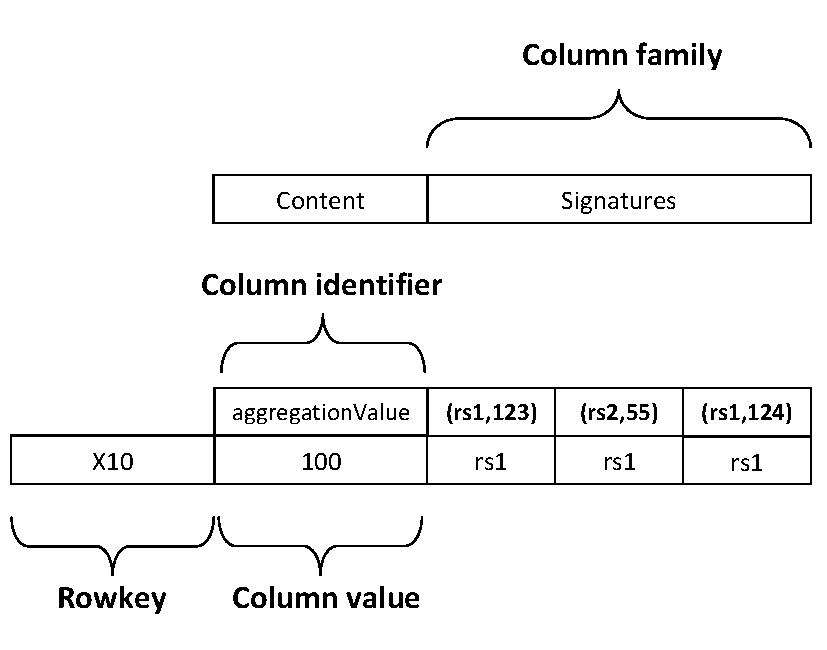
\includegraphics[width=\linewidth]{HBaseRow}
    \caption{HBase Row}
    \label{fig:hbaserow}
\end{figure}


Therefore, we use the possibility of the column based database HBase, to attach arbitrarily columns to one rowkey. In the example, we inserted the update $i_1(R(k2,x1,100))$ to the base table. Now, the corresponding view record $D(x1,50,S)$ is retrieved from the view table. It consists of an aggregation key $x_1$, an aggregation value $100$ and a list of signature records. Figure \ref{fig:hbaserow} depicts the representation of the view record in HBase. The aggregation key uniquely identifies the view records of the sum view. It is stored in HBase as $rowkey$. The aggregation value is persisted by attaching it to a $column\:identifier$, called aggregationValue. In the example, it is just one aggregation value, but in general, there could be several. They are merged under a $column\:family$, named Content.\\ 
In the HBase architecture we can easily derive a global id for the base table updates. A Region Server orders its base table updates using a sequential number $rs_{seqno}$. When an update is written to the Write Ahead Log, the sequence number $rs_{seqno}$ is increased by one. $rs_{seqno}$ is only a local identifier, but if we put it together with the id of the Region Server $rs_{id}$, we receive a global id. For that reason, we use $(rs_{id}, rs_{seqno})$ as the column identifier of a $signature\:record$. It indicates distinctly, if a base table update has already been applied to the view record or not. Additionally, we store the key of the base table operation to the signature record. All signature records are merged under the column family Signatures. When retrieving the view record, we simultaneously fetch all signature records. Since HBase tables work column oriented, the get operation is still fast. Moreover, it is executed atomically and cannot be interfered. To update the view record, we add up the delta value of the base table record. Then, we append a new signature record to the end of the Signature family.\\

\subsection{Wrong update order} 
As mentioned in Section \ref{sec:consistencymodel}, timeliness is an important property of the View Maintenance System. For most classes of views, it is not vital to preserve global order of updates, since it is a requirement for strong consistency. But in the moment, the timeline of a single base table record is changed, even convergence cannot be quaranteed. The following example illustrates this case. 

\noindent 
\emph{Example -- }Consider a selection view with a base table $R(\underline{K},Y)$ and view table $S(\underline{K},Y)$. The view is defined as
\begin{verbatim}
	SELECT K,Y FROM R WHERE Y < 300
\end{verbatim}
There are two updates $u_1(R(k1, 100))$ and $u_2(R(k1, 200))$. View Manager $VM_1$ propagates update $u_1$ and $VM_2$ propagates $u_2$ delivering it faster than $VM_1$. This means the updates are inserted into the base table in right order  but into the view table in wrong order. The final table states are $B_f\{(k1, 200)\}$ and $V_f\{(k1, 100)\}$.

Another example, showing the importance of record timeliness is the following: A join view with two base tables $R_1(\underline{K},X)$, $R_2(\underline{K},Y)$ and view table $S(\underline{K},X,Y)$. 
\begin{verbatim}
	SELECT K,X,Y FROM R1,R2 WHERE R1.K = R2.K
\end{verbatim}
The initial table states are $B_0\{R_2(k1, 200)\}$ and $V_0\{\}$. There are two updates $i_1(R_1(k1,x1,$ $100))$ and $d_2(R_1(k1,x1,100))$. View manager $VM_1$ propagates update $u_1$ and $VM_2$ propagates $d_2$ delivering it again faster than $VM_1$. This means the deletion $d_1$ of the row is delivered before the insertion $i_1$, leading to divergent final states  $B_f\{\}$ and $V_f\{(k1,x1 100)\}$. A diagram of the example is shown in  \ref{fig:co_wrongupdateorderjoin}.\\

\noindent  
\emph{Solution -- }The examples show the importance of record timeliness. In Subsection \ref{subsec:nonidempotentupdates}, we introduced a global id $(rs_{id}, rs_{seqno})$. Anyway, we cannot use this id because, it is just an identifier. It does not introduce a global ordering to updates.  But again, we can rely on the fact, that updates are always written to the Write Ahead Log in local FIFO order. Because updates to the same base table row are always performed locally, we can conclude that local FIFO order is equivalent to record timeliness. This means the whole view maintenance system can guarantee timeliness, if the following two statements hold true.
\begin{itemize}
	\item The updates in the system are always processed in FIFO order
	\item Base table updates to the same rowkey have to be always processed by the same View Manager
\end{itemize}


The first claim is already fullfilled by the architecture of the components. The VM Region Server as well as the View Manager are working with update streams and they are processing the updates sequentially. However, to accomplish the second claim we have to route the updates to the View Managers actively. In the following, we call this mechanism $flow\:control$. To establish flow control and assign the updates consistently, the Update Assigner uses the hash ring. The hash value, which is calculated out of the key of the base table update, remains the same, if the key remains the same. Therefore, multiple updates on a base table record get always assigned to the same View Manager. In Figure \ref{fig:consistentHashing}, key $k_4$ gets always assigned to View Manager $VM_1$. If we calculate the hash value $h(k_4)$ and traverse the hashring in clockwise fashion, then we hit the hash value $h(VM_1)$ of $VM_1$ first.
\begin{figure}[h!]
  
  \centering
    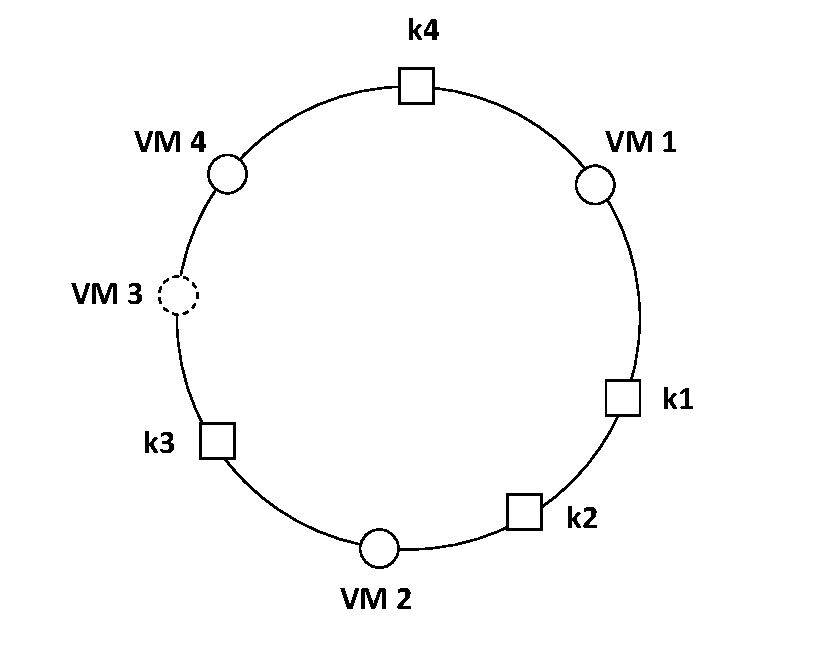
\includegraphics[width=\linewidth]{ConsistentHashing}
    \caption{Consistent Hashing}
    \label{fig:consistentHashing}
\end{figure}

$Flow\:control$ is an easy exercise, as long as we are bound to a static context. In a dynamic context, View Managers can be assinged to or withdrawn from the Region Server. They can crash and be removed from the system. All these processes happen while the stream of updates is continuing. Then, there is a short period of time, in which the order of updates can be changed. Consider an update $u_1(k3, x1, 100)$ taken from the Write Ahead Log and an Update Assigner maintaining the hash ring of Figure \ref{fig:consistentHashing}. The Update Assigner calculates a hash value $h(k_3)$ from key $k3$. The hash value of the View Manager $h(VM_4)$, who is hit first in the hash ring, is determined responsible. Now another View Manager $VM_3$ joins with a hash value $h(VM_3)$, lying between $h(k_3)$ and $h(VM_4)$. The next update $u_2(k3, x3, 150)$ on the same key $k3$ is propagated. The View Manager determined responsible, is now $VM_3$. Taking into account, that $VM_4$ has already queued a lot of updates and $VM_3$ is just processing its first update, we can assume that $u_2$ is likely to pass $u_1$. Again, the record timeline has been broken. To overcome this situation, we establish a control mechanism. If a new View Manager gets registers at the Region Server, then the Region Server put it on the hash ring like in normal operation mode. But the assinged updates of the new View Manager are not delivered.  Instead, the message queue of the new View Manager is put on hold and a marker message $m_1$ is inserted into the stream of all remaining View Managers. The View Managers are processing their update streams and after a while, they entcounter the marker message $m_1$. They react to the message by sending an acknowledgement to the Region Server. After the Region Server has collected all marker messages $m_1$ from the View Managers, it releases the previously queued updates. Now it can be sure, that no update of $k_3$ is still in progress at any of the View Managers.\\   

\subsection{Concurrent commit} 
Our view maintenance architecture aims at a highly parallelizing updates. As we already discovered, we can use flow control to sequentially process updates of a single base table record. But views aggregate the base table data and therefore, updates of multiple base table records are merged together. These updates can of course be processed in parallel. A single view record can be updated by two different View Managers concurrently. This can violate the convergence of a view table as the following example shows.\\ 

\noindent  
\emph{Example -- }Imagine a base table $R(\underline{K},X,Y)$ and view table $D(\underline{X},S)$. The view is defined as
\begin{verbatim}
	SELECT SUM(Y) FROM R GROUP BY X
\end{verbatim}
The initial table states are $B_0\{R(k1,x1,50)\}$ and $V_0\{D(x1,50)\}$. There are two inserts $i_1(R(k2,x1,100))$ and $i_2(R(k2,x1,200))$. View Manager $VM_1$ propagates update $i_1$ and $VM_2$ propagates simultaneously $i_2$. Since the keys of both insert transactions are different, this is not violating the record timeline. Both View Managers retrieve the view record  $D(x1,50)$. Then, they add the delta of their insert operation and write back the view record. Since both view updates are calculate on the same view record value, one of the updates gets lost. In this case, $VM_1$ writes back $D(x1,150)$, then $VM_2$ overwrites the result by putting $D(x1,250)$. The final view table state is $V_f\{D(x1,250)\}$, but it should be $\{D(x1,350)\}$. A diagram of the problem is shown in \ref{fig:co_concurrentcommitsum}.   

\noindent  
\emph{Solution -- }We use $checkAndPut$ methods, provided by HBase, to notice if the value of a view record has been manipulated, while we were calculating the new one. Again consider the situation of the example, when both View Managers have retrieved and calulated the new view records. $VM_1$ writes back its value $D(x1,150)$ to the view table. Likewise, $VM_2$ tries to update the view record, but this time the checkAndPut methods fails. $VM_2$ retries to retrieve and update the view record. It fetches $D(x1,150)$ and calculates $D(x1,350)$. Now the checkAndPut method is successful and $VM_2$ writes back the correct result.\\


\subsection{Update Interference} 
Update interference is a long existing issue in the reasearch of view maintenance. As explained in Section \ref{sec:viewtypes}, there are local and global transactions. Examples for global transactions are the delete operation of a minimum/maximum in a min/max-view or the insert operation of a join view. In case of the min/max-view, we need to compute a new global minum/maximum. In case of the join view, we have to globally query the base table, to determine the matching rows of the join. However, when querying a large set of base table updates, it can happen, that base table records are updated meanwhile. Then the updates are included multiple times. They are in the result of the predecessing query and they trigger an update by themselves. For the min/max-view, this leads to a violation of strong consistency. For the join view, the resulting consistency level depends on, wether the primary keys of the base tables are included in the view or not. If they are included, strong consistency is violated, but weak consistency can be guaranteed. This is related to the fact, that multiple inserts to the same row doesn't change the result. But, if the primary keys are not included, then convergence is violated as the following example illustrates.\\

\noindent  
\emph{Example -- }Imagine two base tables $R(\underline{K},X,Y)$ and  $S(\underline{J},X,Z)$. The view is defined as $D(\underline{X},Y,Z)=R(K,X,Y) \bowtie S(J,X,Z)$. The initial table states are $B_0\{\}$ and $V_0\{\}$. There are two inserts $i_1(R(k1,x1,100))$ and $i_2(S(j1,x1,200))$. View Manager $VM_1$ propagates update $i_1$ and $VM_2$ propagates simultaneously $i_2$. In order to update the view record $VM_1$ has to query the base table. It has to be evaluated if a row of $S$ matches $i_1$. A query to a distributed data set can take a long time and it might happen that update $i_2$ is applied to a Region of the base table before the query of $i_1$ is executed completely. Then the query returns the matching row $D(x1, 100, 200)$. $VM_2$ calculates the join record for $i_2$ and also queries the base table, which yields the same result $D(x1, 100, 200)$. The join record is included twice, producing a final view table state of $V_f\{D(x1, 100, 200), D(x1, 100, 200)\}$.  This violates the requirement of convergence. A diagram of the problem is shown in \ref{fig:co_updateinterferencejoin}\\

\noindent  
\emph{Solution -- }To solve this issue, in \cite{chen:multiversion} the problem of update interference is reduced to the problem of serializing base table transactions at the view table. A global order of base table updates is established by timestamping them with a vector clock. When quering the base table, logical timestamp are used, to retrieve the results. The timestamp indicates the state of the table, when the udpate was applied. The query is then executed on this particluar state of the base table and retrieves the chronological convenient base record version.  If interfering updates exist, they are just excluded from the results. We adapt this concept, nonetheless our context differs from the context in \cite{chen:multiversion}. In \cite{chen:multiversion} the architecture is a centralized Data Warehouse with distributed data sources. Our view table is not centralized, but spread over multiple Region Servers. This means, we cannot serialize the base table operations at view table level, but we can serialize them at view record level. We are storing signature records for every base table update, that has been applied to the base table, in order to detect duplicate updates. We can use the list of signature records to create a logical timestamp. This timestamp can then be taken, to query the base table. Everytime a a record is saved to a HBase table, Hbase produces a new version of it. For that reason, not only the current value, but also the older values can be requested from the table. We restrict the query to return only the versions of base table records, that have a sequence number below the highest sequence number in the signature. In doing so, we exclude all updates that have been issued after the current processed update.

\chapter{Load balancing}
\label{chap:loadbalancing}

In this Chapter, we explain the mechanisms of the system to distribute the work equally among the View Managers, even in a scenario of changing update loads. To achieve this goal, we establish two different kinds of update distribution, local and global load balancing. In both sections, we develop a methodology to measure and calculate the load, in order to change the systems state accordingly.\\  


\section{Local load balancing}

The flow of updates from Region Servers to View Managers can be controlled. This control is always established locally throughout a $subsystem$. The term subsystem refers to a Region Server and the list of View Managers, that are currently assigned to it.\\

\noindent  
\textbf{Update distribution -- }The update distribution from the Region Server to the View Managers is dictated by the consistent hash ring of the Update Assigner. We not only use the hash ring, to consistenly map keys to View Managers and establish flow control. We also use the hash ring to equally distribute the updates. For Consistent Hashing, there is a concept called virtual nodes. If we put just one node on the hash ring for every View Manager, chances are high, that some View Managers get granted a larger key range than others. To overcome this scenario, nodes are replicated in the hash ring. For every View Manager a hash value $h(VM_1)$ is calculated as initial point and from there, a fixed number of points, e.g. hundred, are picked. This helps to minimize the mean variation and achieve an equal distribution.\\ 

\noindent  
\textbf{Load calculation -- }To measure the load distribution within a subsystem we don't care about the load of the Region Server. Instead we are interested in the contingent of updates, a certain View Managers has queued. Ideally, we pick the point exactly after the updates have been pre-processed. Here we know, how many view tables have to be updated. Moreover, this is the last queue before the processing step and we can see how many updates have been accumulated. We calculate  \[load_{VM}(vm)=\sum_{n=0}^{size(queue_{proc}(vm))} numView(queue_{proc}(vm, n))\]If a View Manager is overloaded the update queue indicates it instantly. The View Managers periodically send status messages to their Region Server to report the load.\\  

\noindent  
\textbf{Controlling update flow -- } Especially, when we are using differently powerful network nodes or network connections, this can improve efficiency to a large extent. As mentioned above, we are using virtual nodes within our hashring to equally distribute the udpate load. By modifying the number of virtual nodes, on the hashring, we are able to manipulate the contingent of updates a View Manager receives. We define the contingent of a View Manager by 
$contingent_{VM}(vm)=\frac{numOfVirtualNodes_{VM}(vm)}{numOfVirtualNodes_{subsystem}(rs)}$ 
When the View Manager is put onto the hash ring, for the first time, this should be a fixed number. For example, consider a hash ring with two View Manager $VM_1$ and $VM_2$. Because, we have set the number of virtual nodes to 50, $VM_1$ and $VM_2$ receive a contingent of 50 percent. If a new View Manager $VM_3$ joins again, 50 new nodes are placed on the hash ring, setting the new contingent to 33 percent for each View Manager. Now, in addition to the queued update load we measure the throughput of every View Manager by evaluating the processed updates per second. In order to change the update load of a View Manager, we can adjust the number of virtual nodes. Reducing the number of virtual nodes corresponds to a smaller number of updates assigned to the View Manager, whereas increasing the number virtual nodes has the opposite effect. In order to adjust the virtual nodes, we use the measured load  of a View Manager, devided by the load of all View Managers, belonging to the subsystem 
$loadPercentage_{VM}(vm)=\frac{load_{VM}(vm)}{\sum_{n=0}^{numVM(r)}load_{VM}(vm)}$. 
Since a View Manager should posses a number of virtual nodes, that corresponds to its load, we can set both statements equal $contingent_{VM}(vm)=loadPercentage_{VM}(vm)$. The resulting equality can be used, to determine the number of virtual nodes a View Manager should receive, depending on its update load.

\section{Global load balancing}

Global load balancing is a mechanism, during which the View Managers are assigned to or shifted between the Region Servers. This kind of dynamical view maintenance, should addresses especially the scenario, where one Region Server is heavly flooded by client updates, whereas other Region Servers are not concerned with updates at all. Reassigning a View Manager is bound to a certian cost. Therefore, reassigning View Managers blindly can lead to worse results. We have to measure the load of the subsystems accurately and calculate a load plan.\\ 


\begin{figure}[h!]
  
  \centering
    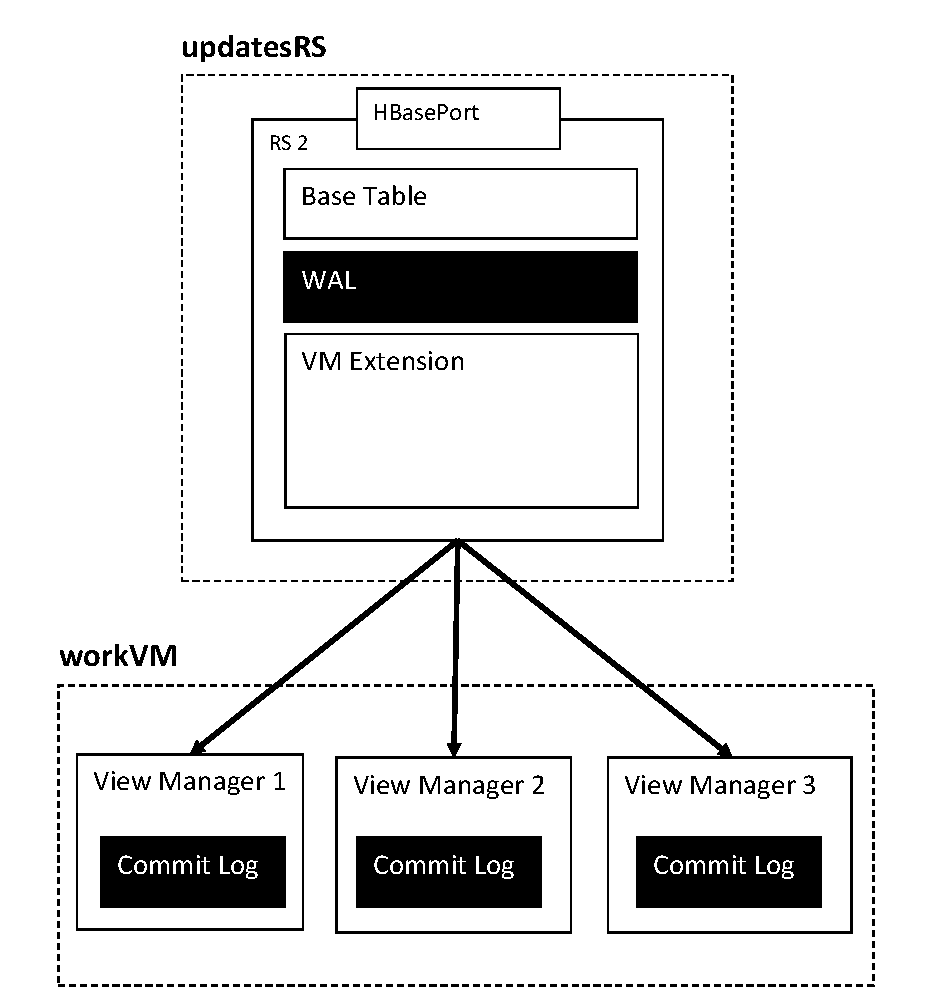
\includegraphics[width=\linewidth]{LoadBalancing}
    \caption{Load Balancing}
    \label{fig:loadbalancing}
\end{figure}

\noindent  
\textbf{Load calculation -- }The first intuitive point, that we use for measuring the systems load is located at the Region Server. Because every update in the process passes the Region Server, we get a complete picture how the loads are distributed. We pick the point where the updates are entering the system. Its right after they are read from the Write Ahead Log and before they are queued for assignment. Then we can determine the number of updates received by the Region Server with equation:
\[updates_{RS}(r)=\sum_{n=0}^{size(wal_r)} numView({wal_r}(n))\]
$wal_r$ denotes the Write Ahead Log of Region Server $r$. ${wal_r}(n)$ returns the nth entry of the Write Ahead Log, containing exaclty one base table update. The number of views, that are defined over the base table relation of the update, is determined by function $numView(u)$. This looks like an easy and efficient approach. The updates are not assigned at that measurement point and therefore we can react to big loads of updates that are flooding a particluar Region Server by simply assigning additional View Managers to it. But the equation doesn't contain any information about how many View Managers are assigned to a Region Server and which amount of work they are serving. As a second point we measure the amount of updates processed by calculating 
\[work_{RS}(r)=\sum_{n=0}^{numVM(r)}size(cl_{r,n})\]
To evaluate the work done at the subsystem, we iterate over all View Managers $n$ assigned to the Region Server $r$ with commit log $cl_{r,n}$. Function $size()$ evaluates the number of updates that a view manager has written to its commit log. Finally we determine the current load that weighs on a Region Server by substracting the amount of work done from the number of queued updates.  
\[load_{RS}(r)=\frac{updates_{RS}(r)- work_{RS}(r)}{numVM(r)}\]
Now we have derived an accurate number of the amount of updates that are burdened on a subsystem, containing of a Region Server and its assigned View Managers. To implement the load measurement the View Managers are continously sending status reports to the Region Server. The report contains the number of updates that have been processed and written to the commit log. The Region Server on the other hand, calculates the load of the subsystem and sends a status report to the master. Based on the status reports the load balancer component of the master makes a descision how the View Managers should be distributed. There are five events the load balancer has to react to: View Manager/Region Server added, View Manager/ Region Server removed and a general load balancing. The latter can be performed periodically to relieve a heavy loaded Region Server or to reassign View Managers sitting idle.\\


\noindent  
\textbf{View manager increased -- }When a View Manager is added to the system, it is idle by definition and needs to be assigned to a Region Server. Before we assign the View Manager, we analyse the systems state. In order to find a Region Server, we exercise two different rounds of selection. In the first round, we select all Region Servers that haven't got a View Manager and whose update count in the Write Ahead Log is larger than zero. We want to avoid at all cost, that there is a Region Server with already queued updates and no View Manager to process them. If no region Server of that kind is found, we look in the second round for the Region Server with the highest update load. If there are multiple Region Servers with a maximum load, one is picked out of the resulting set randomly. The process is shown in Figure \ref{fig:lb_addviewmanager}.\\
\begin{itemize}
	\item First round, look for blocked Region Servers:
\[\{r \in R \mid updates_{RS}(r) > 0 \wedge numVm(r) == 0\} \]
	\item Second round, look for heaviest loaded Region Server:
\[\{r \in R \mid load_{RS}(r)== max(load_{RS}(r_1),..load_{RS}(r_n))\} \]
\end{itemize}


\noindent  
\textbf{View manager decreased -- }When a View Manager is removed or crashes, the View Manager count is decreased. If it hasn't been the last View Manager of the affected Region Server, then nothing is done. If it was the last View Manager of the Region Server and updates are still queued, then we have to ensure again, that the stream of updates is not blocked. We select the least loaded Region Server with more than one View Manager and reassign it to the affected Region Server. The process is shown in Figure \ref{fig:lb_removeviewmanager}.
\begin{itemize}
	\item First round, determine if affected Region Server is blocked:
\[updates_{RS}(r) > 0 \wedge numVm(r) == 0\]
	\item Second round, depending on first round, do nothing or search View Manager from least loaded subsystem and reassign it:
\[\{r \in R \mid load_{RS}(r)== min(load_{RS}(r_1),..load_{RS}(r_n))\} \]
\end{itemize}

\noindent  
\textbf{Region server increased -- }When the Region Server count is increased, we have to assure that the newly added Region Server is not blocked. The scenario is similar to the case $View$ $Manager$ $decreased$, if a Region Server loses its last View Manager. Therefore we take the exact same counter measures. We just substitute the affected Region Server with the newly added one. The process is shown in Figure \ref{fig:lb_addregionserver}.\\

\noindent  
\textbf{Region server decreased -- }When a Region Server crashes, there can be several free View Managers that have to be reassigned. The scenario is similar to the case $View$ $Manager$ $increased$. But now we can have more than one View Manager, therefore we execute the steps of $View$ $Manager$ $increased$ multiple times, until no free View Managers are left. The process is shown in Figure \ref{fig:lb_removeregionserver}.\\

\noindent  
\textbf{General load balancing -- }When we are doing the standard load balancing, two rounds are performed again. In the first round, we look for least and the heaviest loaded subsystem, respectively. First, we caclulate the current $throughput$. Then, we calculate $throughput^*$, which we get by taking a View Manager of the least loaded subsystem and reassigning it to the heaviest loaded subsystem. Finally we compare $throughput < throughput^*$ to find out if a reassignment of a View Manager would improve the systems overall performance.   
First round:\\

\begin{itemize}
	\item First round, determine least and heaviest loaded subsystem:\\
$\begin{array}{ll} rmax & \in R_{max}  =\{r \in R \mid\\& loadRS(r)== max(load_{RS}(r_1),..load_{RS}(r_n))\} \end{array}$

$\begin{array}{ll} rmin & \in R_{min}  =\{r \in R \mid\\& loadRS(r)== min(load_{RS}(r_1),..load_{RS}(r_n))\} \end{array}$
	\item Second round, compare loads of reassignment:\\
$load_{RS}(r_{min}) + load_{RS}(r_{max}) < load_{RS}(r_{min}^*) + load_{RS}(r_{max}^*)$
\end{itemize}

\chapter{Failure Detection}
\label{chap:failuredetection}

Failure detection and automatic recovery plays a critical role for distributed view maintenance. In a scenario, where we scale up to hundreds of network nodes, we cannot rely on manually actions, to restart components or clean up data inconsistencies. The components, that are scalable in our system are View Managers and Region Servers. For that reason, we model a crash scenario for both component types and formulate appropriate counter measures.\\
 
\noindent  
\textbf{Crash of master -- }The crash of the master component is a special case because the master does not lay on the update path and it is just a single unit. However if it crashes we  handle the case like HBase is dealing with a master crash. There is no way of running multiple master at a time, but regardless of that multiple master can be started. Only the master who first contacts the Zookeeper and establishes its session node, is the operating master. The others are just backup masters contacting the Zookeeper periodcally. If the current master crashes one of the waiting backup masters overtakes by using the persistently stored system configuration.\\ 

\section{Crash of View Manager}

When a View Manager crashes, the Region Server, who is sending updates, doesn't notice anything. For the sake of perfomance, the View Manager does not acknowledge the update messages. The Region Server is just firing the updates to the View Managers.  
But as mentioned above, the View Manager has registered to Zookeeper by creating an ephemeral node. This means, the active session of the View Manager is monitored. The timeout, after an View Manager is declared crashed, can be specified. If the View Manager has crashed, its ephemeral node is destroyed. Since the master has registered an observer to the View Manager branch, it gets informed by Zookeper. In Figure \ref{fig:viewmanagercrash} the process is shown. \\

\begin{figure}[h!]
  
  \centering
    \includegraphics[width=\linewidth]{SO_ViewManagerCrash}
    \caption{View Manager crash}
    \label{fig:viewmanagercrash}
\end{figure}

To record its work state, the View Manager is equipped with a Commit Log. The Commit Log is located in a directory of the distributed file system HDFS. It is represented by a replicated logfile, named after the viewmanager. After each processed entry, the View Manager writes the transaction to the Commit Log. If the View Manager has crashed, the Commit Log contains the last processed update. 

Nevertheless, sending the updates to the View Manager is usually a lot faster, than the View Manager can process the updates. Hence, a lot of updates can be waiting in the queue of the View Manager. In case of a crash, all the updates in the queue are lost. As mentioned above, the VM Master is informed when the View Manager crashes. The Event Processor of the master creates an event and passes it to the Recovery Manager. The Recovery Manager opens the Commit Log of the crashed View Manager. If it finds already processed transactions, it evaluates the transaction with the highest sequence number. 

In the next step, the Recovery Manager of the VM Master sends two messages to the responsible Region Server via the Component Controllers interface. The first message contains a withdraw View Manager command, such that the Region Server deletes the View Manager from its hashring and stops sending updates to it. In the second message, the Recovery Manager sends a command to the Region Server, advising it to replay the Write Ahead Log. Upon receiving the replay command, the Region Server activates its WAL Reader component to reset the pointer of the Write Ahead Log. From the current position, the WAL Reader sets the pointer to the position of the highest sequence number, retrieved before.

Now, the Region Server starts replaying and resending the updates from the position, where the View Manager crashed. As a downside, some of the View Managers, who are working properly have to process some of the udpates twice. But due to the fact, that we are using signatures, non-idempotent udpates are not a problem. Likewise, the record timeline can be quranteed.



\section{Crash of Region Server}
Exactly like the View Manager, the Region Server is registred at the Zookeeper service. If the Region Server crashes, the VM Master is notfied by Zookeeper. As a first step the master does a look up in the system configuration, to discover which View Managers are currently assigned to the crashed Region Server.  Then, it sends a message to the View Managers, informing them about the crash of the Region Server. Now, the View Managers act similar to the withdraw command. They wait until all the updates in their queues have been worked off. After the updates are finished, the View Manager extracts the sequence number of the last processed update and sends it to the VM Master. If by chance, one of the View Managers crashes as well, the VM Master is aware of it. It just reads the sequence number from the Commit Log. Subsequently, the VM Master compares all collected sequence numbers and determines the smallest one. It has to use the smallest number, to eliminate the possiblity of updates getting lost. The VM Master reassigns all View Managers to a new Region Server. Finally, it advises the new Region Server to replay the updates from the smallest sequence number, retrieved before.


\chapter{Implementation}
\label{chap:implementation}

In this Chapter, the architecture, designed in Chapter \ref{chap:architecture}, is realized. First, the parts of the implementation are discussed, that concern the whole architecture.  The communication between the components, the integration with HBase as well as Zookeeper. Then, in the following Sections, implementations of individual components are picked, that have been particular challenging. For example, the implementation of the subcomponent WAL Reader, is explained in detail. 

\section{Components}

Figure \ref{fig:implementationoverview} shows a small setup of the View Maintenance System. In the top right, there is the VM Master component, controlling the system. In the top center, there is a Region Server, holding two update queues, which are serving a View Manager, respectively. In the bottom of Figure \ref{fig:implementationoverview}, there are two View Managers, which are processing the updates. Every component possesses a Controller subcomponent, that manages it. The Controller subcomponent is initialized during creation of the component. It starts the other subcomponents in single threads. As you can see in Figure \ref{fig:implementationoverview}, the subcomponents are connected by three little squares in most cases. The squares represent queues, that are implemented as buffers between the components. They buffer base table updates, as well as communication messages, that are sent between the components. The following example illustrates, how the queues are working, to build a conveyor of updates. The WAL Reader subcomponent of the Region Server runs in a single thread. It connects to the HDFS and pulls updates from the Write Ahead Log. It puts the update to a queue, which is simultaneously the input queue of the successor component. The queues are implemented by a class called $ConcurrentLinkedQueue$. This class ensures mutual exclusion upon access to the data. Because two threads from different sides are accessing the data structure concurrently, this a necessary requirement. The class owns two methods $push$ and $pull$, whereas $push$ inserts an element at the beginning of the queue and $pull$ retrieves and deletes an element from the end of the queue. Using the queues, every subcomponent thread can work at its own speed, that it is able to achieve. This prevents the subcomponents from being flooded with updates and most important, the updates are always kept in the right order. However, tests of the system have showed, that, if queues are running too full, the subcomponent begins slowing down constantly. For that reason, the preceding subcomponent can respect a certain limit. In case the output queue of the predecessor reaches this limit, it stops working and waits until the size of the queue has droped again.


\begin{figure}[h!]
  
  \centering
    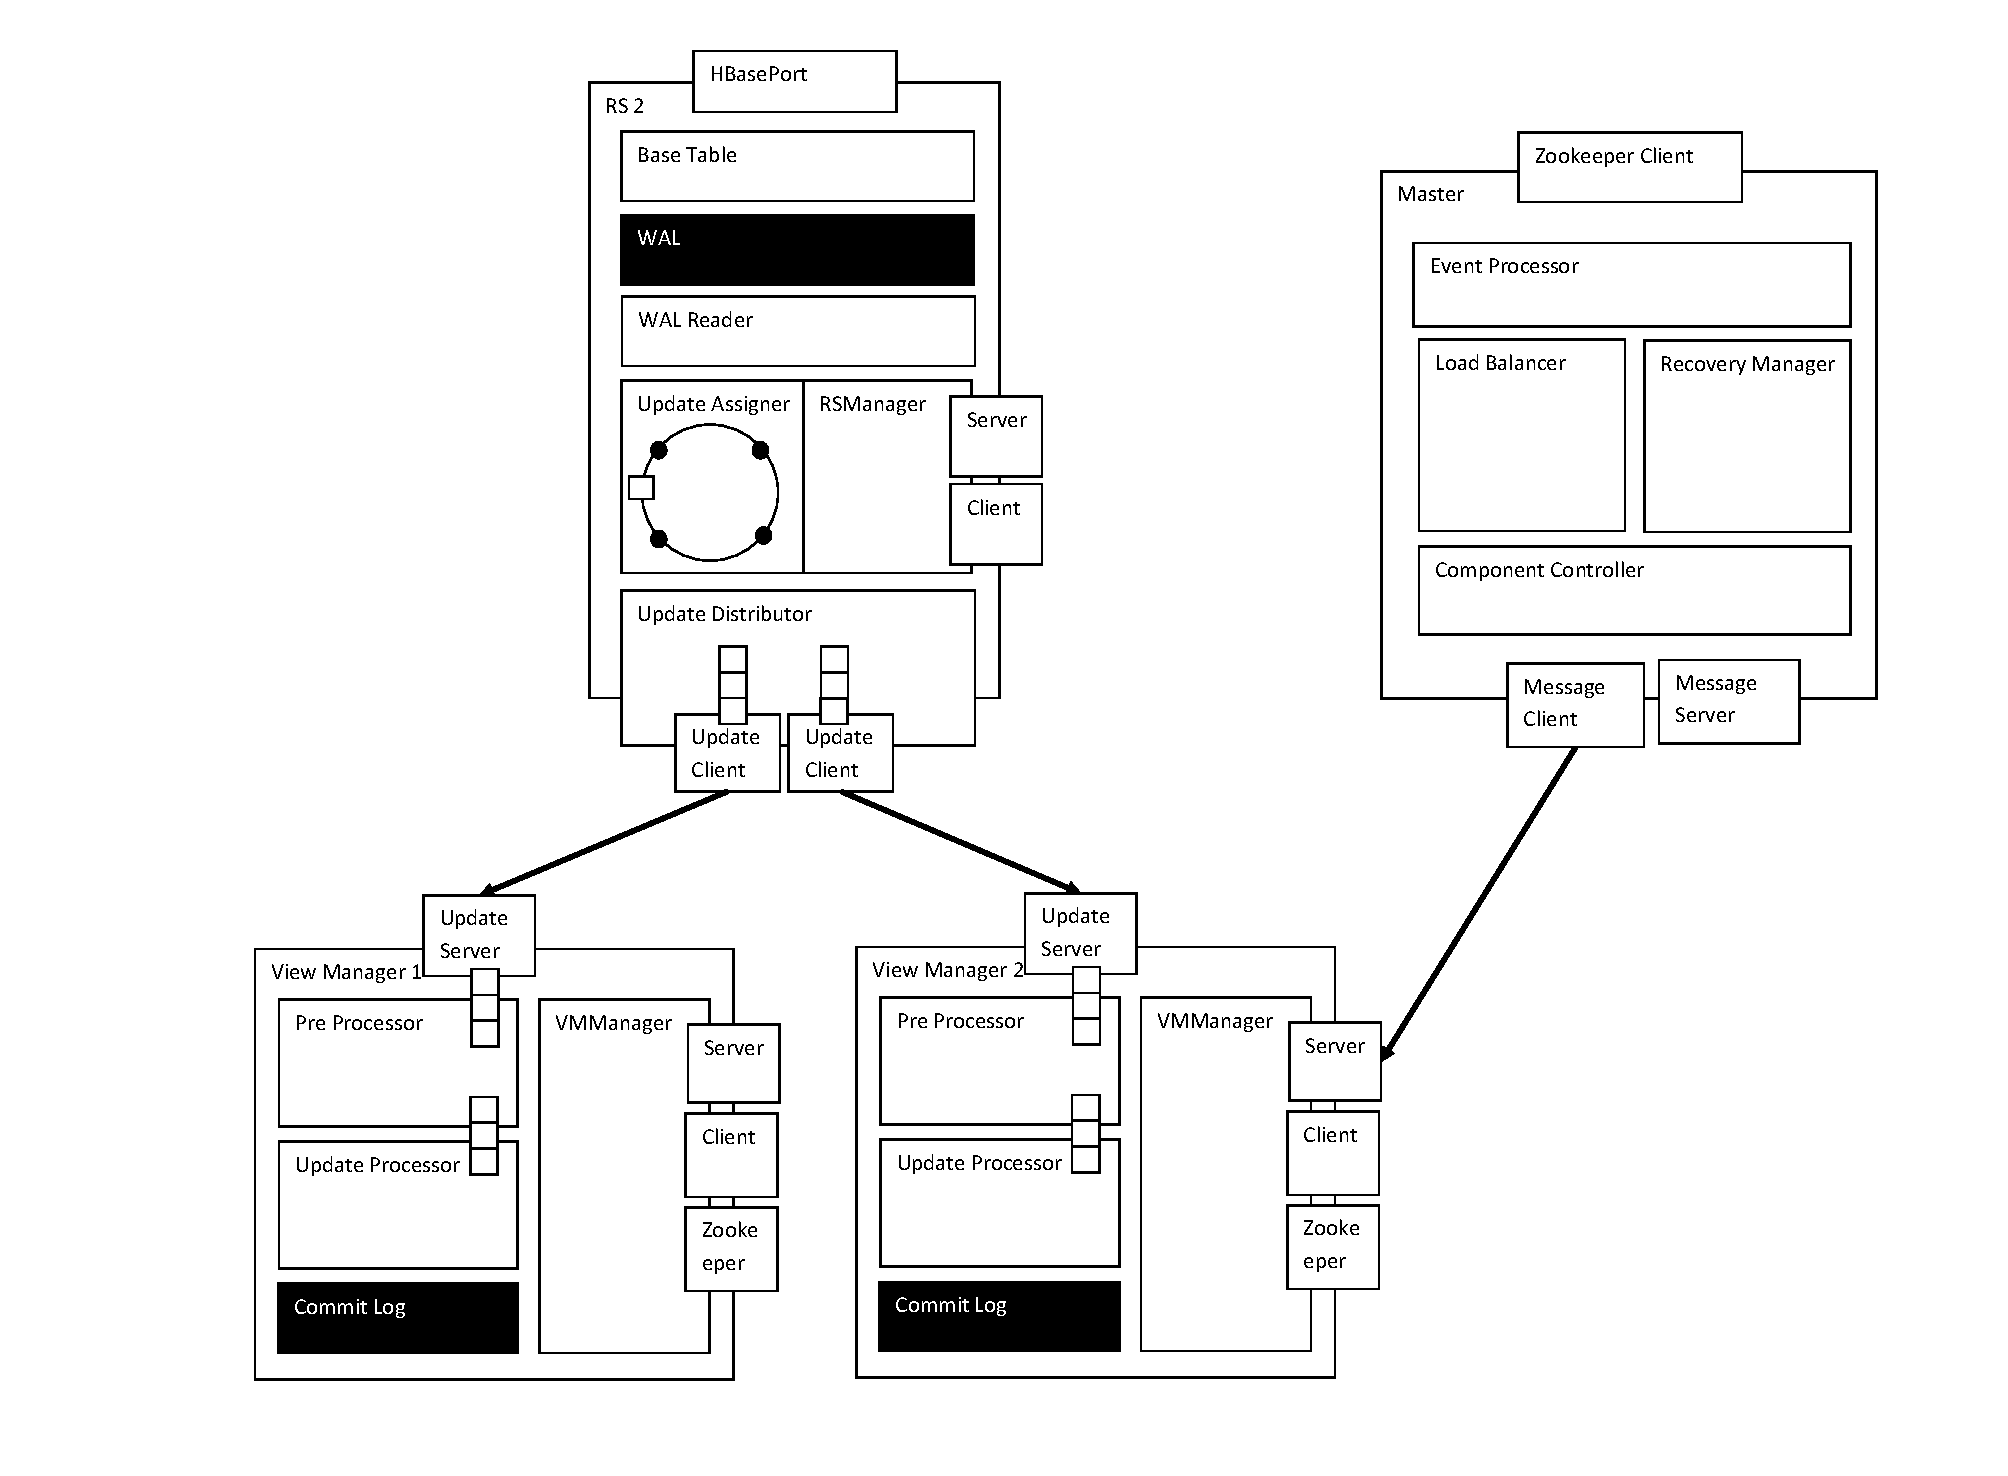
\includegraphics[width=\linewidth]{ImplementationOverview}
    \caption{Implementation Overview}
    \label{fig:implementationoverview}
\end{figure}


\section{Communication}

We implement the communication between the components with the help of sockets. For that reason, there are always two roles of communication. The sender of a message runs a client socket. The client socket opens a tcp connection to a certain address/port and hands over its request. The receiver of the message runs a server socket. The latter is listening on a defined port of the hosting machine. When the server socket accepts a client call, it passes the call to a separate thread. Then, the thread processes the client request. In order to communicate properly, the components have to always implement the client and the server side of the communication. Because, the way components communicate in the system is identical, we only have to implement a $Client$ and a $Server$ class for all components. In addition to the communication roles, there are two types of communication between the components. One type of communication is the $update\:flow$, the other type is the $message\:flow$. The two types differ in the messages they exchange, but also in the way they communicate. Therefore, we implement two different handler classes for both types. The update flow is established by the classes $UpdateClient$ and $UpdateServer$, whereas the message flow is realized with the help of the classes $MessageClient$ and $MessageServer$. 


\subsection{Update Flow}
The update flow is always a one-directional communication from a Region Server to the View Managers. The main purpose of the update flow is to push as many updates through the communication channel as possible. Therefore, the protocol of the update flow doesn't provid acknowledgements. In order to send the updates, the Region Server creates an individual update queue for every assigned View Manager. Then, the Region Server starts an instance of the class $UpdateClient$ in a single thread. The thread just pulls updates from the update queue and sends them to the $UpdateServer$ object. The $UpdateServer$ object receives the updates and puts them to an update buffer. The updates are sent in form of string messages. To use the full bandwith of the tcp channel, a message is always filled up to a fixed size. It can happen, that multiple updates are send within a message, as well as, that only one half of an update is sent. For that reason, the updates have to be reassambled at the side of the $UpdateServer$  object. To denote the start and the end of and update, we use the letters '$<$' and '$>$'. The update string stores the properties of the $BaseTableUpdate$ class in the following format. $<baseTable;regionServer;type;rowkey;col1=val1,col2=val2;oldcol1=oldval1,oldcol2=oldval2>$. The letter '$;$' separates the single parts of the message. The field $rowkey$ stores the key of the base table update. After the rowkey, two variable message parts follow. The first message part stores the columns and their values, that have been set in the update operation. There can be arbitrary columns for a rowkey and therefore, the columns and their values are separated by the letter '$,$'. The second variable part corresponds to the first part, but it stores the old values, which were found at the rowkey, before the base table update was applied. In case of an insert operation, the part with the old values is empty. For update operations, both variable parts are filled. Considering the delete operation, the first part, containing the new values, is empty.

\subsection{Message Flow}

The message flow is established in order to exchange information between the components. In most cases, the communication is initiated by the VM Master. In contrast to the update flow, the message communication is bi-directional. Every message is acknowledged by the receiver, to ensure, that it has been processed. If a message is not acknowledged, the sender tries to resend the message several times. After a fixed number of tries, the sender gives up and proceeds with other communication messages.  The messages correspond to the following format: $<component;systemID;command/event;params>$. The field $component$ specifies the type of the sending component. In the View Maintenance System, there are three types:  VM Master, VM Region Server, View Manager. The second field $systemID$ allows the component, to be identified and addressed uniquely, in the entire system. The system ID again, corresponds to a certain format: $<name;ip;messagePort;$ $updatePort>$. For example, the system ID of a View Manager could be $<vm1;192.168.0.20;$ $4555;4666>$. If a component registers at Zookeeper in the beginning, it does so by using the system ID. This way, the VM Master instantly knows, that it has to send the commands to the IP address $192.168.0.20$ on port $4555$. Likewise, a Region Server knows, it has to send the updates to IP address  $192.168.0.20$ on port $4666$. Considering again, the format of the messages, there are two more fields: $command/event$ and $params$. The field $command/event$ specifies either an command or an event. Most of the commands, that are implemented, are derived from Section \ref{sec:systemoperations}. There are additional commands for failure recovery. With the help of commands the VM Master instructs the components to execute the transferred action. For the commands, sometimes extra params are required. They are stored into the field $params$ and divded by the letter '$:$'.  In Table \ref{tab:commands}, an overview of the systems commands is given.

\begin{table}[h!]
\begin{center}
\begin{tabular}{ l l l}
  command & sender & receiver \\  \hline
  assignViewManager & Master & View Manager \\
  withdrawViewManager & Master & View Manager \\
  withdrawCrashedViewManager & Master & Region Server \\
  resassignViewManager & Master & View Manager \\
  shutdownViewManager & Master & View Manager \\
  replayWriteAheadLog & Master & Region Server \\
  startUpdateProcessing & View Manager & Region Server \\
\end{tabular}
\end{center}
\caption{Commands}
\label{tab:commands}
\end{table}

Instead of a command, an event can be put into the message. An event informs the receiver about an action, that has taken place in the system. Usually, to kinds of events are sent to the Master. The first kind are the Zookeeper events, that inform the Master about creation and deletion of components. The second kind are component events, that acknowledge the commands, the Master has given previously. Both kind of events are processed at the Master and lead to subsequent commands. In Table \ref{tab:events} an overview of the system events is shown.




\begin{table}[h!]
\begin{center}
\begin{tabular}{ l l l}
  command & sender & receiver \\  \hline
  rsAdded & Zookeeper & Master \\
  rsCrashed & Zookeeper & Master \\
  rsShutdown & Zookeeper & Master \\
  vmAdded & Zookeeper & Master \\
  vmCrashed & Zookeeper & Master \\
  vmAssigned & View Manager & Master \\
  vmWithdrawn & View Manager & Master \\
  vmReassigned & View Manager & Master \\
  vmShutdown & View Manager & Master \\
  crashedVmWithdrawn & Region Server & Master \\
  statusReportVm & View Manager & Region Server \\
  statusReportRs & Region Server & Master \\
  markerReceived & View Manager & Region Server \\
\end{tabular}
\end{center}
\caption{Events}
\label{tab:events}
\end{table}


\section{Zookeeper Integration}

\begin{figure}[h!]
  
  \centering
    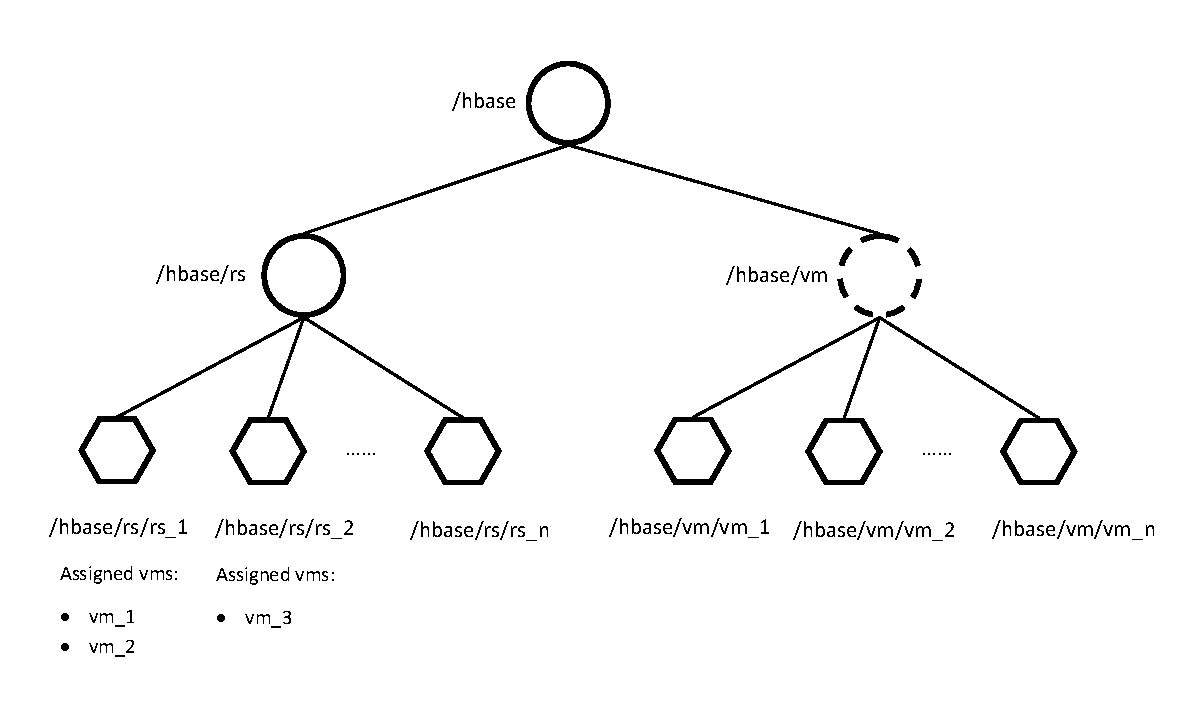
\includegraphics[width=\linewidth]{Zookeeper}
    \caption{System model in Zookeeper}
    \label{fig:zookeeper}
\end{figure}

Like explained in Section \ref{sec:zookeeper}, the coordination service Zookeeper is used to de-, register components and to detect crashes in the View Maintenance System. Zookeeper keeps the current system configuration by storing a model of the system.  In Figure \ref{fig:zookeeper} the data structure of the system model is shown. Persistent nodes of Zookeeper are depicted by a cirlce, whereas ephemeral nodes are represented by a diamond. The root node is referenced by path $/hbase$. HBase creates it automatically when starting up the system. The left branch can be reached by path $/hbase/rs$. In this directory HBase creates a node for every Region Server, e.g. $/hbase/rs/rs1$. The nodes of the Region Servers are ephemeral. This means they are created when a Region Server starts up and joins the HBase cluster. If a Region Server performs a shutdown or crashes, then the node is destroyed immediately by Zookeeper. Ephemeral nodes are always bound to a session of a client and Zookeeper controls the liveliness of clients by sending heartbeat messages periodically. In HBase every node can store additional information in a small text file. We use this ability to store a list of View Managers within every Region Server node. This way, the assignment of View Managers to Region Servers is persisted safely, into Zookeeper. Stored information in Zookeeper is replicated, so even in case the master crashes, the system configuration is still available. Another master can start up, access the configuration and continue controlling the system. The right branch of Figure \ref{fig:zookeeper} is added for view maintenance purposes only. It is a persistent node, which is referenced by $/hbase/vm/$. When the VM Master starts up and the node is not existing, it creates a new one. In case, there are old session nodes in $/hbase/vm/$, the VM Master cleans them up. During startup every View Manager creates an ephemeral node, e.g. $/hbase/vm/vm1$. Similar to the Region Servers, the node is deleted as soon as the View Manager leaves the cluster. 
In order to realize the described functionality, the API of Zookeeper has to be used.  The VM Region Server and the View Manager components use the same Zookeeper functions to register themselves. Therefore, we implement one Zookeeper Service for all components. The service provides the procedures $createSessionNode$, $deleteSessionNode$ and $nodeExists$. With the help of $nodeExists$, the component checks, whether it has already been registered. If yes, the component aborts startup with an appropriate message. If no, the component executes $createSessionNode$. 
The VM Master controls the View Maintenance System. It does so by reacting to events, that occur in the system. The subcomponent, which is responsible for collecting the events, is the Event Processor. The Event Processor implements the $ChildrenCall$ interface of Zookeeper. On startup the Event Processor is registered to the $/hbase/rs$ and the $/hbase/vm$-node of Zookeeper. In case, children of these nodes are removed or added, Zookeeper performs a callback to the Event Processor. It executes the method $processResult$ of the $ChildrenCallback$ interface and hands over an up-to-date list of children. The Event Processor compares the list with the last copy it received and creates a new event, e.g. View Manager $vmAdded$. Then, the Event Processor passes the event to the Load Balancer for further processing. Everytime, the Event Processor receives a notification, it has to register at Zookeeper again. Zookeeper supports this asynchronous type of event processing, to achieve high performance and scalability and to avoid unneeded subscriptions.
     

\section{HBase Integration}

\subsection{Reading WAL Records}
\label{subsec:readingthewal}

In Section \ref{sec:systemcomponents} we explained, that the WAL Reader component of the VM Region Server retrieves the updates from the Write Ahead Log of the underlying distributed file system HDFS. To implement access to the Write Ahead Log, we have to use the client API of HDFS. But as a start, we have to understand how HBase manages its logs files in HDFS. Figure \ref{fig:hdfs} shows a hierarchic view of the folders, starting with the root directory of HBase. In the root directory, there is a directory called $.logs$. In that directory a subdirectory for every Region Server is created by HBase. The name of the subdirectory consists of the address, the port number of the Region Server and a hash value. Here the Write Ahead Log of the Region Server can be found. There is always one Write Ahead Log for one Region Server. The Write Ahead Log itself is a package of multiple log files, that are named after the Region Server, plus an additional hash value. If a log file exceeds a certain size, a new log file is started. As mentioned in Subsection \ref{subsec:nonidempotentupdates} all update entries, that are written to the log files, receive a unique sequence number by HBase. HBase uses the sequence number to identify, which updates have been flushed to disk already. If a log file contains only updates, that have been written to the table already, it is deleted. The WAL Reader component uses the sequence number as pointer to the Write Ahead Log. Because of the pointer, the WAL Reader knows, where it has read the last update entry.\\

\begin{figure}[h!]
  
  \centering
    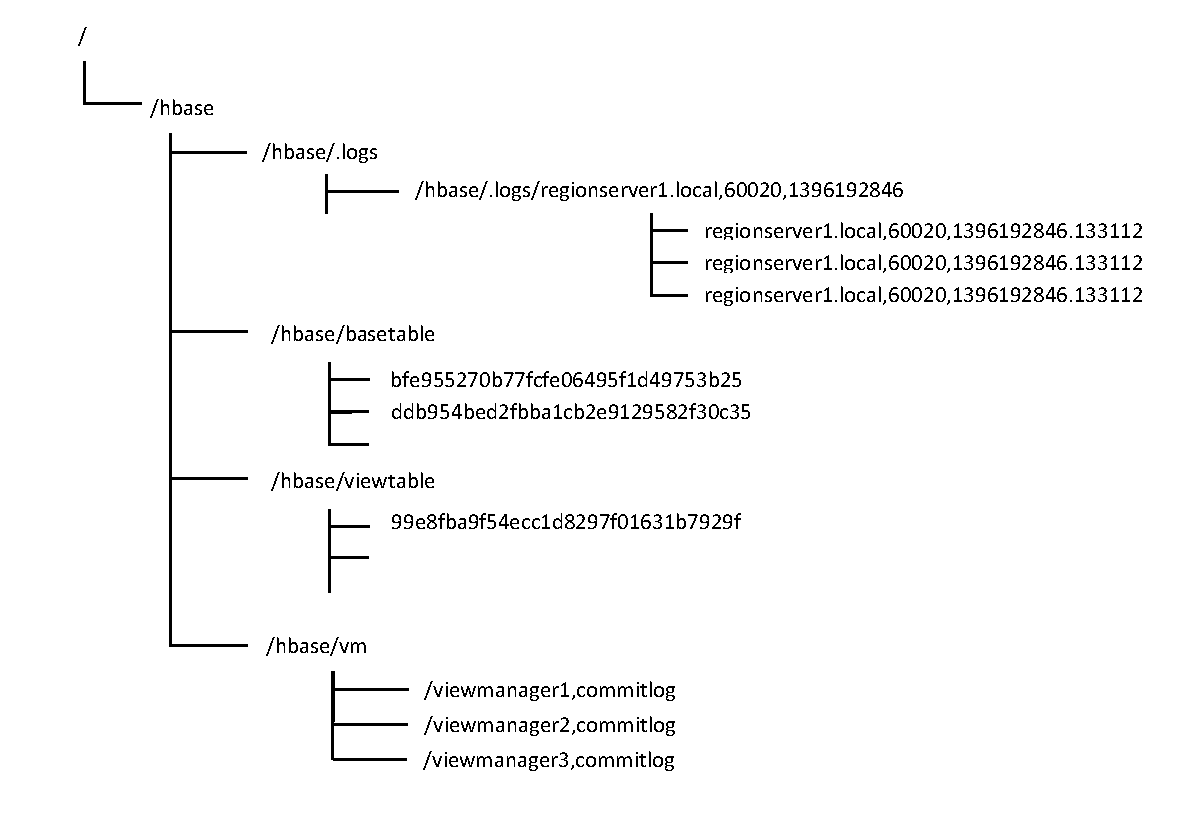
\includegraphics[width=\linewidth]{HDFS}
    \caption{Directory Structure in HDFS}
    \label{fig:hdfs}
\end{figure}


For every table in the data base, there is a directory in the root folder of HBase. For the View Maintenance System, this means one directory for the base table and one directory for the view table, as depicted in Figure \ref{fig:hdfs}. The table directory contains a subdirectory of every table region, named with the hash value of the region keys. The table regions can be hosted on different Region Servers and for that reason, the Region is stored independently of the Region Servers. Every table entry, that has been written to the WAL and is inserted into the Memstore, is flushed to disk after a while.  Then it is written to the table file in the Region directory of the base or view table. 


In the constuctor, the WAL Reader receives the address of HDFS and the address of the Region Server, it is placed on. In order to extract the client updates from the WAL, the WAL Reader connects to the HDFS and reads out all subdirectories of the $/hbase/.logs$-directory. The subdirectory, whoose name contains the Region Server address, is selected as base directory. Then the WAL Reader iterates all log files, it finds in the base directory. The log file is read by using the $SequenceFileLogReader$ class of HBase. The $SequenceFileLogReader$ retrieves a WAL entry for every client update. The WAL entry consists of a $HLogKey$ and $WALEdit$ object. Like a key of a table, referencing a certain value, the $HLogKey$ references a WAL entry. It contains the sequence number and the name of the table, the update was made to. The $WALEdit$ object represents the logged client operations. It contains a list of $KeyValue$ objects, because the client is able, to update multiple columns of rowkey, at a time. These updates are executed automatically and therefore, persisted to only one log entry. Moreover, the $KeyValue$ object contains the type of operation. Insert and update operations are tagged with put, delete operations are tagged with delete. 

\subsection{Forwarding WAL Records}

To forward the WAL entries, the WAL Reader creates a $BaseTableUpdate$ object, whoose properties are shown in Figure \ref{fig:basetableupdateobject}. This object is filled with the information, that is needed by the View Manager, to further process the update. For example, the name of the base table is the first property of the object. The View Manager needs it to resolve the view tables. The Region Server name and the sequence number are properties to uniquely identify the update, later. Moreover, the type of operation is included, to determine, if a base table update should be added or deleted from the view table. Finally, the $BaseTableUpdate$ object holds the rowkey and a list of new values, as well as the list of old values. In Figure \ref{fig:basetableupdateobject} a base table operation of type update is shown. The list of old columns represent the state of the base table row before the update, whereas the list of new columns represent the current state. Both column sets are needed by the View Manager, in order to calculate the view delta.

\begin{figure}[h!]
  
  \centering
    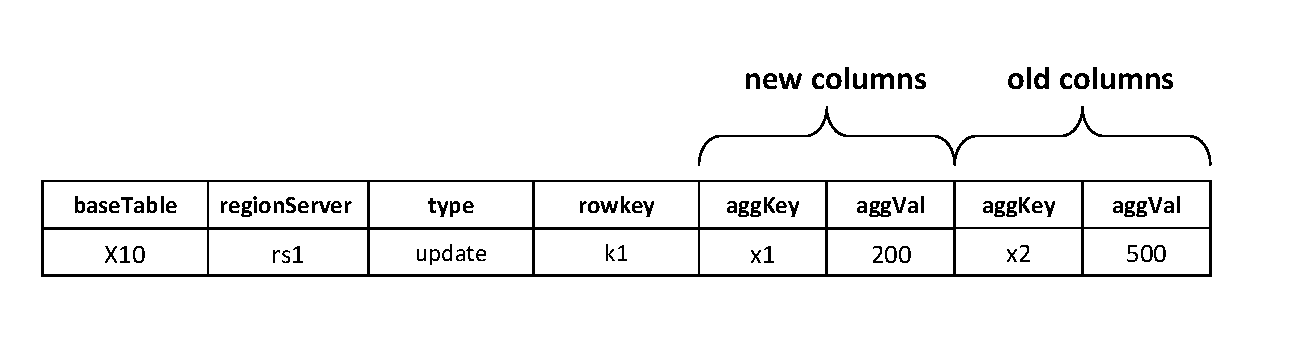
\includegraphics[width=\linewidth]{BaseTableUpdateObject}
    \caption{BaseTableUpdateObject}
    \label{fig:basetableupdateobject}
\end{figure}



In the example of Figure \ref{fig:basetableupdateobject}, the following problem arises. The client sends the rowkey and the new values, together with the operation type put. Using the Key-Value Store API, the client doesn't care, whether the put is an insert or an update operation. In the example, it is an update operation, so the View Manager has to know the old values of the rowkey, that have been updated. But the base tables updates are written to the Write Ahead Log of HBase, before they are inserted into the tables. When retrieving an update from the Write Ahead Log, the former history of the rowkey, that is updated, is not reflected. Therefore, the old columns are not included in the WAL entry. A similar situation appears, when the client deletes a rowkey. It just sends the command $delete\:key$, but the View Manager has to know the values of the row, before it was deleted.

To solve the problem we take an approach, that uses update hooks. As stated in Section \ref{sec:alternatives}, update hooks can be used in HBase, to execute a piece of code, before HBase operations are performed. This can be any kind of data manipulation and definition operations, e.g. put, get or create, drop table.  We use a method called $preWALEdit$. It is called on every Region Server separately, before a client update is written to the Write Ahead Log. The entry, that is going to be written to the WAL, is handed over as a parameter. Additional information can be added to the entry, that will be also persisted to the Write Ahead Log. Like mentioned above, when peforming delete and update operations, the WAL entry is missing the information about the former values. In order to complete the missing information, we perform a local get operation on the rowkey. We don't perform a get using the standard HBase API. This would imply getting routed from zookeeper to the Region Server in three steps. In a distributed storage system, we want to avoid global operations. We already know, that the key of the update operation is located on the Region Server, which is running the $preWALEdit$ method, anyway. Therefore, we use the local context of the Region Server, that is given in the $preWALEdit$ method, instead. The local context helps us, to retrieve the old values and they are put into the WAL entry, together with the rowkey and the new values. These values are later retrieved by the WAL Reader and forwarded to the View Managers with the help of a $BasesTableUpdate$ object.


\subsection{Log Cleaning}
Another implementation problem, that has to be solved, refers to the log cleaning mechanisms of HBase. To not stress the hard disk capacity of the servers, HBase cleans out old logs. If HBase detects, that all entries of a WAL log file, have been flushed to disk, then this file is deleted. This is a worst case scenario for the View Maintenance System because updates could be lost. It would mean, that calculated views are inconsistent, instantly. Again, we make use of the HBase features to overcome the problem. HBase offers the possiblity to replicate database transactions from one HBase cluster to another. Because the replication should be applied immedeatly after the point in time, at which the database update can be considered safely, the entries of the Write Ahead Log are taken. The problem appearing during replication is the same. Log files could be deleted and the replication is then incomplete. For that reason one can override the Basic Log Cleaner class and define own criteria,  that decide about the deletion of a log file. We implement an extended Log Cleaner class and define the criterion as follows. If the processing of the update with the highest sequence number in the log file has been confirmed, then the file can be deleted by HBase. The Log Cleaner class is located at the Region Server, but the Updates are processed at the View Managers. That's why we need to send a sequence number, indicating that the update has been processed, from the View Managers to the Region Server. 

\section{Commit Log}

A Commit Log is written by every View Manager in the system. Like shown in Chapter \ref{chap:failuredetection}, the Commit Log is needed to recover from possible crashes. The entries of the Commit Log should be persisted safely. Therefore, the same approach as for the Write Ahead Log of HBase is chosen. The HDFS API is accessed and the Commit Log is written to the underlying distributed file system. Here, it can be replicated over the nodes of the network. But, there is also a difference to the Write Ahead Log. In the Write Ahead Log one base table udpate results in one log entry. Considering the work of the View Managers, base table updates are multiplied by the number of views, that have been defined over the relation. One base table update can result in hundreds of view table updates. For that reason, one base table update results in multiple log entries in the Commit Log. In case of a crash, the next View Manager can continue the work at exact the point, where the crashed View Manager abandoned the Commit Log. Figure \ref{fig:hdfs} shows how a $/hbase/vm$-directory is created in the root directory of HBase. This is achieved by the VM Master, calling the function $mkdirs$ of the HDFS client API. The directory is then used by the View Managers. Every View Manager connects to HDFS by itself. It creates a Commit Log file and starts adding entries, as new updates arrive. Because the Commit Log works exactly like the Write Ahead Log, the View Manager uses the $SequenceFileLogWriter$ class of HBase. The class enables the View Manager to sequentially put $WALEdit$ objects to the log. The $WALEdit$ objects are referenced by $HLogKey$ object, just like explained in Subsection \ref{subsec:readingthewal}. In addition to the WAL, the $HLogKey$ consists of the view table name, together with the base table name and the sequence number.
     



\chapter{Evaluation}
\label{chap:evaluation}

In this Chapter we present the results of our experiments. We design an evaluation environement, that is reused for every experiment. Afterwards, we conduct seven types of experiments to evaluate effects of different parameters on the systems performance. We describe the results and interpret the meaning of them.  \\

\section{Experiment setup}
\subsection{Deployment}
Our experiments are performed on a cluster of 40 nodes, running on a compute server (Ubuntu 12.10, 4 x Intel Xeon 4650 @ 2.70GHz 8 cores, 32 x 16GB RAM, 2 x 800GB SSD/4 x 1,2 TB HD). We use 11 nodes, to install the Apache Hadoop distribution. The Hadoop Distributed File System builds the bottom layer of HBase, where the data of tables and logs is stored to files. HDFS consists of two types of nodes. The namenode stores metadata and processes the routing requests, when a client contacts the file system for the first time. Similar, to the Master of HBase, there is only one namenode in the system. The data node is the unit of scalability. Like the HBase Region Servers, the data nodes store the replicated files and process the file requests of the clients. In a typical setup, there is one master and ten data nodes. The recommendation of Apache is, to choose exactly as many data nodes as Region Servers. Moreover, a Region Server should always be located at the same machine as the corresponding data node. This is, because HBase prefers writing to a local data node, instead of going for a remote data node. Using locality improves performance to a great extent. In our tests, we made a contradictory and surprising observation. With increasing number of data nodes the performance started slowing down. This might be related to the hard drives of the cluster. Instead of using one hard drive per node, we rely on two SSDs for the whole cluster. This means, if we increase the number of data nodes, then we do not gain the i/o-performance of another hard drive, but instead we write to the same hard drive at different points. To not hurt the performance of the system, we use one master node and one data node on a single machine, respectively. The HBase Master is hosted on the same machine as the HDFS name node. In contrast to the HDFS configuration we initiate multiple Region Servers in the HBase system. Because a Region Server is bound to a certain limit of requests, spreading the requests to different nodes, helps to improve performance. In order to examine the influence of Region Servers we changed the setup, going from one Region Server up to eight instances. On every Region Server node, we deploy the extended functionality like defined in Subsection \ref{subsec:vmregionserver}. It is deployed in form of a java program. At startup, the java program connects to HDFS and begins reading the Write Ahead Log of the Region Server, it is hosted on. As soon as View Managers are added to the hash ring, the program starts propagating updates.  The View Managers are hosted on 20 separate nodes. They are also deployed in form of a java program. We do not always use the full contingent of View Managers, depending on the experiments, that we run. For a proper evaluation, we have to take at least as many View Managers as Region Servers. Otherwise, there are Region Servers that are not able to propagate their updates. Another 8 nodes are reserved for the client application, issuing update operations to HBase. We take 8 clients to generate a high degree of parallelization during update generation. We want to evaluate how the Region Server of HBase perform under heavy update load. Furthermore, the paralellization shortens the creation of the database to a great extent. Especially, when putting a million base table records and more, this is critical. 


\subsection{Table configuration}
\label{subsec:tableconfiguration}
At the start of our experiments, we create one emtpy base table and a set of empty view tables. If a base table update is propagated, every view table has to be updated, separately. The assignment of view tables to the base table and the definition of the views are put to an extra table, named $view\:definitions$. The view definition table is read by the View Managers on startup, so that they know the views they have to update. The view tables have the following view types: count, sum, min and max, selection and k-fk join views. 

We want the base table updates, to be equally distributed among the amount of Region Servers, we define in the experiments. By default configuration, HBase stores all base table records at the same Region Server in one Region. In the moment the Region grows to large, it is split into two Regions and one Region is moved to another Region Server. For our experiments the updates have to be equally distributed. Therefore, we use the option HBase to preconfigure the Regions of the base table. HBase handles the assigment of Regions to Region Servers by itself. For that reason, we cannot assign fixed Regions to the Region Server. Instead, we pre-split the base table and rely on the load balancer of Hbase to equally assign the Regions to the Region Servers. To increase the probability of an equal distribution, we can of course raise the number of Regions. If we have exactly as many Regions as Region Servers, chances are high, that one Region Server gets assigned two Regions while another is sitting idle. But, if we split the table into more Regions, e.g. 10 Regions per Region Server, then the spreading of Regions is very smooth and equal.

For the view types count, sum, min and max we create a column in the base table, called aggregationKey. This column corresponds to the column, that is usually preceeded by a GROUP BY clause in sql statements. The column indicates, which columns should be aggregated. It is the primary key of the view table. The second column is named aggregationValue. This column contains the values, that are counted, summarized, etc. Because we want to use a specified number of aggregation keys, we choose a random number between 1 and a upper bound. The upper bound determines the number of aggregation keys during evaluation. The random number is then appended to x. Likewise, the aggregation values are generated randomly, within a specified range. For the selection view we use the same base table. We just forward the entries of the base table. As selection condition we take the aggregationValue. The k-fk join view needs two base tables. For that reason we create two tables with different primary keys. The primary key of the right table is stored to a column in the left table, called foreignKey.

\section{Workload}

The workload, we generate consists of insert, update and delete operations, that are issued to HBase via the client API. Depending on the view type, the insert operations contain a key and a set of columns. For the first block of experiments, we create an equal distribution of update keys. In order to do so, we need to make the following preparations. 


In case the Regions are equally distributed to the Region Servers, we have to take care that the same number of base table updates is applied to every Region. This can only be achieved by generating the primary keys, appropriately. Consider a table with 100 entries and 5 Regions. The key ranges would be k1 - k20, k21 - 40,...,k81 - k100. By generating insert operation with random keys in the range of k1..k100, we would achieve an equal distribution of update operations. But HBase compares primary keys bitwise. The key k1 e.g., is greater than key k11. For that reason, we get different Region sizes. We have to always use the same number of digits. In the example, we take k001 and k011. Now, the keys are compared correctly and the Region sizes are equal.

During our experiments, we primarily evaluate the performance of the system. Consistency is evaluated on a theoretical basis in Chapter \ref{chap:viewconsistency}. Despite of that, we check the convergence of every view table in the experiment. We precompute a correct view while creating the base table. This precomputed version of the view table is finally compared to the end result, calculated by the view managers. This way we can ensure, that at least the results are correct at the end of the experiment.


In the first set of experiments, we fill the base table by applying a set of 1.000.000 insert operations to the base table. After the base table operations have been issued, the base table contains exactly the same amount of records 

\section{Performance metrics used}
\label{sec:performancemetricsused}

In order to evaluate the performance of the View Maintenance System, we measure performance indices at defined points. The indices are measure at every Region Server, as well as every View Manager. The measures are taken within intervals of a second and written to a statistic log. After every run, the logs are collected for evaluation. The following indices are measured at the Region Server. \\\\
\textbf{Region Server indices:}
\begin{itemize}
	\item $updatesRetrieved$ The total number of updates, that haven been retrieved from the Write Ahead Log
	\item $queueSizeIncoming$ The size of the queue, that stores the WAL entries before they are processed by the Region Server
	\item $updatesAssigned$ The total number of updates, that have been assigned to View Managers by the UpdateAssigner.
	\item $queueSizesOutgoing$ The sizes of the transfer queues, that are created per View Manager. The number indicates how many updates are wainting to be sent to a View Manager.
	\item $updatesSent$ The total number of updates, that have been sent to View Managers.	
	\item $updatesProcessingTime$ The total processing time the Region Server needed to retrieve and send all updates
\end{itemize}
The total numbers of updates show accurately, how many updates have been processed at a certain step in the processing chain of the Region Server. From the numbers we can derive other indices. For example the $updatesAssignedPerSecond$ are build by subtracting the amount of $updateAssigned$ of the last second from the $updatesAssigned$ of the current second. This value nicely visualizes the throuput of the Update Assigner subcomponent. The queue sizes also show an important aspect, that cannot be expressed by the total numbers of updates. They show, how many updates are waiting to be processed by the next subcomponent and help to identify possible bottle necks. Moreover, results of the evaluation showed, that queues, which are flooded heavily with updates, slow down the system, additionally. This was a reason, to implement certain limits at which a predecessing subcomponent stops working, to not overload the successor. In the following, the perfomance indices of the View Manager are shown.\\\\
\textbf{View Manager indices:}
\begin{itemize}
	\item $queueSizeIncoming$ The size of the queue, that is buffering the updates, sent by the Region Server
	\item $updatesReceived$ The total number of updates, that have been received from the Region Server
	\item $updatesPreProcessed$ The total number of update, that have been pre-processed. Pre-processing stands for evaluating the view definition on the updates base table. Depending on the amount of view definitions on the base table the number of updates is multplied after this step. If there are two views defined, then the number of updates, that have to be processed, doubles.
	\item $queueSizeIntermediate$ The size of the queue, that buffers updates between the pre-processing and the processing step
	\item $updatesProcessed$ The total number of updates, that have been processed. Processed updates have been applied to the view, but they are not written to the commit log 
	\item $updatesProcessedPerSecond$ The same as updatesProcessed, but only the number of updates in the last second
	\item $updatesCommitLog$ The total number of update, that have been acknowledged to the commit log.
	\item $updatesProcessingTime$ The total processing time, the View Manager needed to receive and commit all updates
	
\end{itemize}





\section{Summary of control parameters}
Depending on the intention of the experiment, the following control parameters are varied. In order to clearly show the effects of the parameter, in most of the experiments only one parameter is changed.
\begin{itemize}
	\item $numberOfClients$ The number of clients, that are sending update operations to HBase in parallel. The higher the number, the higher the load, that is put on the Region Servers		
	\item $numberOfRegionServer$ The number of Region Servers, that are configured for HBase at startup. 
	\item $numberOfViewManager$ The number of View Managers, that can be assigned to Region Servers in an experiment. The number has to be equal or greater than the $numberOfRegionServers$ because else some of the Region Server cannot propagate their updates and the evaluation run cannot be finished
	\item $numberOfUpdateOperations$ The number of update operations, that are generated and send to HBase by the clients. Every client generates the amount of $numberOf$ $UpdateOperations/numberOfClients$ update operations
	\item $typesOfUpdateOperations$ This parameter defines which types of update operations are generated by the clients. The three possible types are: $insert$,$update$ and $delete$
	\item $numberOfBaseTableRegions$ The number of Regions that are pre-configured for the base table. The number should be chosen with regard to the parameter $numberOf$ $RegionServer$ like explained in Subsection \ref{subsec:tableconfiguration} 
	\item $numberOfViewTableRegions$ The number of Regions, that are pre-configured for the view tables. The number of Regions that are pre-configured for the base table. The number should be chosen with regard to the parameter $numberOfRegionServer$ like explained in Subsection \ref{subsec:tableconfiguration}  
	\item $numberOfAggregationKeys$ The possible number of aggregation keys, that are chosen in case of sum, count, min and max view types. The number determines, out of which range the random number are chosen, in order to generate the aggregation key. The parameter should be chosen with regard to the number of created base table records. The factor $numberOfCreateBaseTableRecords/numberOfAggregationKeys$ finally decides how many base table records are assigned to one view table record. If there are many base table records, many View Managers might be processing requests to the same view record. 
	\item $numberOfAggregationValues$ The range of values, that are aggregated
	\item $typesOfViews$ The types of views, that are used for the evaluation run. Possible types are $count$, $sum$, $min$, $max$, $selection$ and $join$.
	\item $numberOfViews$ The number of view tables, that is created for every view type. This parameter allows the creation of, e.g. hundred view tables, that are assigned to a base table
\end{itemize}



\section{Execution}
\label{sec:execution}

During evaluation we found out, that one Region Server gets overloaded by the clients update operations. For that reason, the minmal configuration is two Region Servers. To ensure, that the updates of both Region Servers get propagated, we use two View Managers. We start HBase and create the base tables, the view tables, as well as the view defintions. If the tables already exist, they are just cleaned. Then, we start the VM Master and the View Managers on their node, respectively. They get assigned automatically to the Region Servers. The context of the first experiments is static, meaning, that the View Managers are assigned in the state of zero updates propagated. A dyamic context would mean to start the View Managers, when the clients have already started putting their update operations. Then, the View Managers would be attached smartly to the Region Servers with the heaviest load. In the static context, the View Managers are just distributed, equally. 

In the next step, we let the clients put the specfied amount and type of update operations to HBase in parallel. Now, the Region Servers start propagating the updates and the View Manager start updating the views. Every, second the View Manager write to their statistic log, as described in Section \ref{sec:performancemetricsused}. When the Region Server doesn't receive updates anymore, it queues a marker update for every View Manager. In the moment the View Manager process the marker update, they stop the processing time and send an answer to the Region Server. If the Region Server has collected the markers of all View Manager it sends an confirmation message to the VM Master. After all Region Servers have confirmed completion, the VM Master begins the last phase. Shutdown messages are sent to all components. The logs and the statistic logs are collected from all nodes and stored in a directory. Now the system is ready to start the next cycle of the experiment. The number of View Managers is increased by one. The experiment is repeated until we reach the maximum of twenty View Managers. Now, the same 19 cycles are repeated for another view type. In the moment all view types are evaluated we stop the experiment.


\section{Experiment 1}
\label{sec:experiment1}


In the first experiment, we want to evaluate the maximal throughput of the View Maintenance System. We want to show, that we can improve the throughput of the system, significantly, by increasing the number of View Managers. If we attach multiple View Managers to a Region Server, the Region Server distributes the updates equally among the View Managers. For every new View Manager, that is attached, the throughput should increase by a linear factor. Furthermore, we want to conduct the experiment for every view type. This way, we want to compare how the different view types perform in terms of throughput and scalibility. In order to determine the throughput of the View Maintenance System, we take a look at the View Managers. The number of updates, that all View Manager write to their commit log corresponds to the number of updates, the system was able to process. Since, we are interested in throughput and not in absolute numbers, we calculate the average throughput of a View Manager as follows. 
\[avg\_throughput_{vm}(vm)= \frac{updatesCommitLog(vm_n)}{updateProcessingTime(vm_n)}\] 
The average throughput of the whole system then evaluates to.
\[avg\_throughput_sys(sys)=\sum_{n=0}^{numVM(sys)} avg\_throughput_{vm}(vm_n)\] 
We use a data set of 1.000.000 insert operations.  We use only insert operations on aggregation views, because this is the simplest type of view operation. It does not involve table scans or multiple operations on the view table. We can exlusively test the performance of scalibility and neglect effects, dedicated to the operation types. The operations are distributed uniformly among the primary keys of the base table. In Figure \ref{fig:throughput}, the results of the experiment 1 are shown. On the x-axis, the number of View Managers is shown. Every point denotes a cycle of the experiment. On the y-axis, the average throughput of the complete View Maintenance System is depicted. The throughput is measured in calculated view records per second.

\begin{figure}[h!]
  
  \centering
    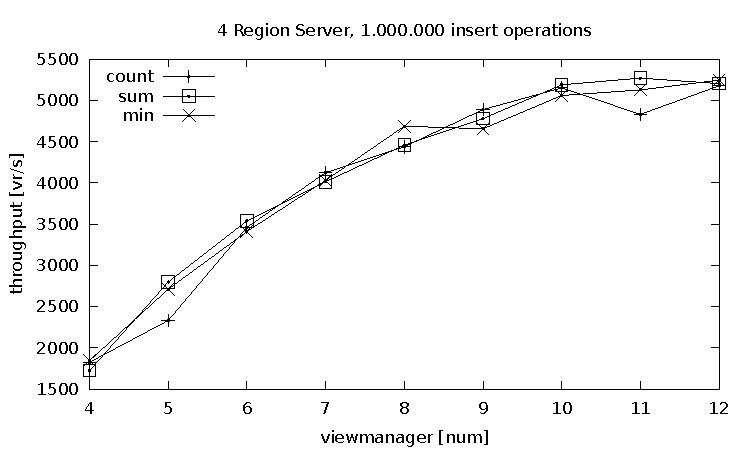
\includegraphics[width=\linewidth]{Throughput}
    \caption{Results Experiment 1}
    \label{fig:throughput}
\end{figure}

As Figure \ref{fig:throughput} shows, we are able to increase the overall throughput of the system from 1500 view records per second to 5500 view records per second, just by adding more View Managers. We make the observation, that the throughput of the system increases nearly linear up to a point of eight View Managers. Then, the effect of parallelization begins to diminish. In the beginning, every new View Manager achieves an additional throughput of 600 - 700 view records per second. This is the maximum number of updates a View Manager can process in the system. By increasing the number of View Managers to ten and more, the additional throughput develops negatively from 700 to 100 view records per second. We are able to exclude the subcomponents of the VM Region Server as reason for this effect. The Write Ahead Log as well as the Update Assigner and the Update Distributor work at a speed of approximately 50.000 updates per second. This is enough speed, to feed at least 50 View Managers in parallel. The bottlneck of the update flow is located at the point, where the View Managers access the view. Changing the number of Region Servers or splitting the view table does not reduce the effect. We think, that the decrease of performance is related to the server cluster, we use for evaluation. We rely on virtualization of the nodes, that are hosting the View Managers. Different nodes of the server cluster write to the same hard drive. Therefore, the limit of hard drive accesses is reached at a certain point and we cannot scale up anymore. In theory, we could futher increase the throughput linearly by adding View Managers with real additional hard disc capacity.



\section{Experiment 2}
\label{sec:experiment2}

In experiment \ref{sec:experiment1} we have shown the effect of scalability. Now, we want to differentiate the effects of the different view types. For that reason, we are using a mixed workload, consisting of insert, update and delete operations. Different update operations of different view types are treated differently by the View Managers as explained in \ref{sec:viewtypes}. Therefore, we expect varying impacts on the different view types. We use a data set of 1.000.000 insert, update and delete operations. The operations are distributed uniformly among the primary keys of the base table. In Figure \ref{fig:throughput_uniform}, the results of the experiment 2 are shown. On the x-axis, the number of View Managers is shown. Every point denotes a cycle of the experiment. On the y-axis, the average throughput of the complete View Maintenance System is depicted. The throughput is measured in calculated view records per second.

\begin{figure}[h!]
  
  \centering
    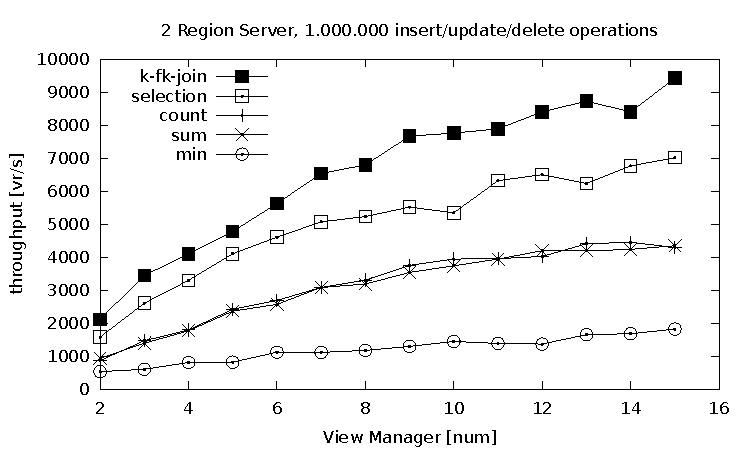
\includegraphics[width=\linewidth]{Throughput_uniform}
    \caption{Results Experiment 2}
    \label{fig:throughput_uniform}
\end{figure}

The results show, that the k-fk-join view performs best. At a first glance, this is a very surprising result because join views have to access the base tables for every insert operation. But in case of the k-fk-join view, the calculation of the view table is different. On insert operations at the left table, the right table is only accessed by the primary key. No table scan is required. Insert and delete operations to the right table do not trigger any processing at all, because the key-foreign-key constraint avoids it. The selection view is also very fast, because the base table updates are just forwarded to the view, depending on a particular condition. The condition decides about the performance of the selection view. Like for the k-fk join, the view maintenance is sped up by those operations, that do no require a view table update. If the selection condition excludes eighty percent of the base table records, then processing only takes place in twenty percent of the cases. The view is very fast. If the condition excludes only ten percent, the selection view is slower but still faster than a count view.

 In Figure \ref{fig:throughput_uniform} the performance of sum and count is nearly equal. This is dedicated to the fact, that the operations of both view types are equal. The only difference is, that in the sum view, we add and substract the value of the base table operations, whereas in the count view, we add and subtract a one. Aggregation views have to calculate every base table operation. There aren't any cases, where no processing is done, like in the k-fk and selection view. Considering the aggregation views, the View Manager has to execute two recalculations for every update operation. One recalculation to subtract the old aggregation value and one recalculation to add the new aggregation value. The min view performs worst, because it is the only view in the test setup, which has to execute table scans. Complete table scans are very expensive. If the min views is configured to provide a lot of aggregation keys, then the minimum value of a particular aggregation key is likely to be deleted. For that reason, the performance of the min view is strongly depending on the number of aggregation keys. We could add a join view to the test setup, where the tables are joined on non-primary keys of both base tables. Then, the performance would be similar to the min view, because the join view would have to execute a lot of table scans, too.




\section{Experiment 3}
\label{sec:experiment3}

In this experiment, we want to evaluate the maximal throughput of the View Maintenance System under unequal update loads. For that reason, we create a load of update operations, that have a higher probability to be stored on a certain Region Server. Instead of a uniform distribution, we use a zipfian distribution on the primary keys of the base table. This means, the closer a key is to the start of the key range, the higher the probability, that an operation is created there.

\begin{figure}[h!]
  
  \centering
    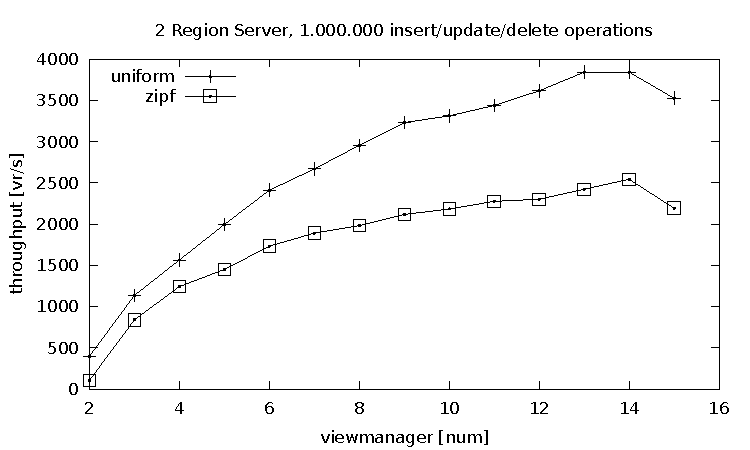
\includegraphics[width=\linewidth]{Throughput_zipf2}
    \caption{Results Experiment 3}
    \label{fig:throughput}
\end{figure}

In the static context, as explained in \ref{sec:execution}, the system doesn't react to the changing update load and some of the View Managers are idle, while others are heavily working. This results in a lower throughput of the View Maintenance System. The more View Managers are used, the more View Managers are sitting idle with regard to the Zipf distribution. For that reason, the effect is intensified at the right side of the diagram.




\section{Experiment 4}
\label{sec:experiment4}


In this experiment, we want to evaluate the effect of different sizes of operation sets to the View Maintenance System. In \ref{sec:experiment1}, we used one million update operations. In productive enviroments, a Large Scale Distributed Database has to handle every size of data sets. We want to evaluate the effect on the system, in a scenario of increasing update operations. We start with a set of 10.000 update operations and increase the number by factor 10 each iteration. The number of Region Servers is two, the number of View Managers remains fixed at eight. We expect the system to handle every update load. Moreover, the throughput of the system should be idependent of the applied load. It should only depend on the number of View Managers, that are available. Naturally, the time to build the view should raise by using a larger data set.

\begin{figure}[h!]
  
  \centering
    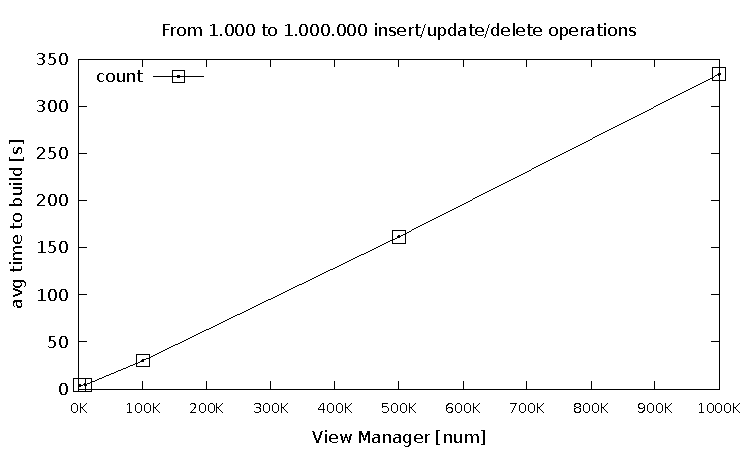
\includegraphics[width=\linewidth]{DifferentDataSize}
    \caption{Results Experiment 4}
    \label{fig:differentdatasize}
\end{figure}

In Figure \ref{fig:differentdatasize}, the results of experiment 4 are shown. On the x-axis, the number of operations is shown, that have been applied to the base table. On the y-axis, the average time to build the view table is depicted. It is measured in seconds. Like expected, the time to build the view increases linearly with the size of the data set. It doesn't matter, if we issue a small or a large set of operations to the base table. The View Maintenance System starts processing the updates at the maximal throughput, it can achieve. In case nothing unexpected happens, the systems keeps the throughput until the processing has finished.


\section{Experiment 5}
\label{sec:experiment5}

In this experiment, we want to evaluate the effect of different numbers of aggregation keys to the aggregation views. The less aggregation keys we use, the more base table updates are mapped to a view record. In scenarios, where we use many View Managers, the probability of contention should increase, significantly. Likewise, the performance is influenced, negatively. To evaluate the effect, we vary the number of aggregation keys. We start at the number of records, which represents a one-to-one mapping and reduce the number of aggregation keys to a minimum of 1000. We expect a decrease in performance, when many View Managers are updating few view records. In this moment, a lot of contention should arise.


\begin{figure}[h!]
  
  \centering
    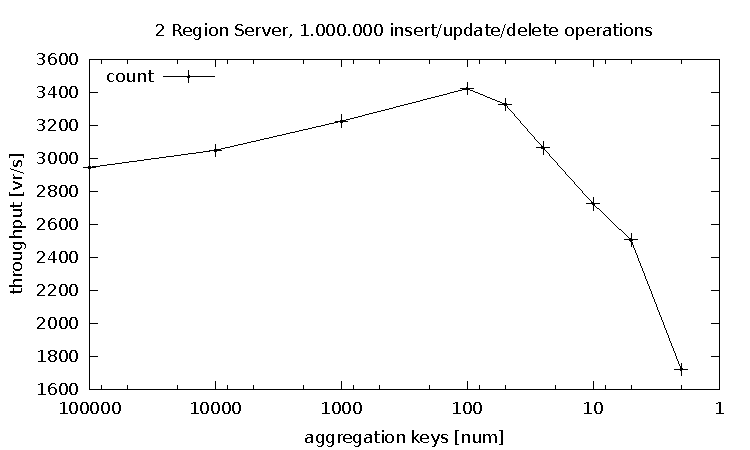
\includegraphics[width=\linewidth]{AggregationKeys}
    \caption{Results Experiment 5}
    \label{fig:aggregationkeys}
\end{figure}

In Figure \ref{fig:aggregationkeys}, the results of experiment 5 are shown. On the x-axis, the number of aggregation keys is shown, that are generated. We reduce the number of aggregation keys and start from 100.000, going down to 2 aggregation keys. Because the the effect is the strongest at the end, we use a logarithmic scale. On the y-axis, the average time to build the view table is depicted. It is measured in seconds. On the y-axis, the average throughput of the complete View Maintenance System is depicted. The throughput is measured in calculated view records per second. Obviously, the curve in Figure \ref{fig:aggregationkeys} rises in the range between 100.000 and 100 aggregation keys. Because the aggregation key is the primary key of the aggregation view, a smaller number of aggregation keys reduces the size of the view table. A smaller size improves the access times to the view table and for that reason we can witness the effect. Around 100 aggregation keys, the performance begins to drop significantly. Here, we record a large gain in view record contentions. Like stated above many View Managers are accessing few view records. In most cases, they have to wait until they are allowed to update the view. 

\section{Experiment 6}
\label{sec:experiment6}

Like the base tables, the view tables can be split into Regions and distributed over the Region Servers. If a view table is distributed, it can be accessed in parallel. As a downside, the routing of the clients is more costly. In \ref{sec:experiment1} we didtn't split the view table. Now, we apply different split factors to the view table and evaluate the effect on performance. We expect a slight increase in performance, even the effects should't be as important considering the dimensions of the test setup. We use a fixed setup of two Region Servers. In addition we use four View Managers for experiment 6a, as well as eight View Managers for experiment 6b. We apply a set of 1.000.000 insert, update and delete operations to the base table. In both experiments, we start with a view table, that is not splitted. Then, we increase the number of view table Regions after every iteration. We stop the experiment at split factor of ten view table Regions.

\begin{figure}[h!]
        \centering        
		\begin{subfigure}{0.49\textwidth}  
%    		\includegraphics[width=\textwidth]{ViewTableSplit}
    		\caption{Results Experiment 6a}
    		\label{fig:viewtablesplit}
		\end{subfigure}
		\begin{subfigure}{0.49\textwidth}   
    		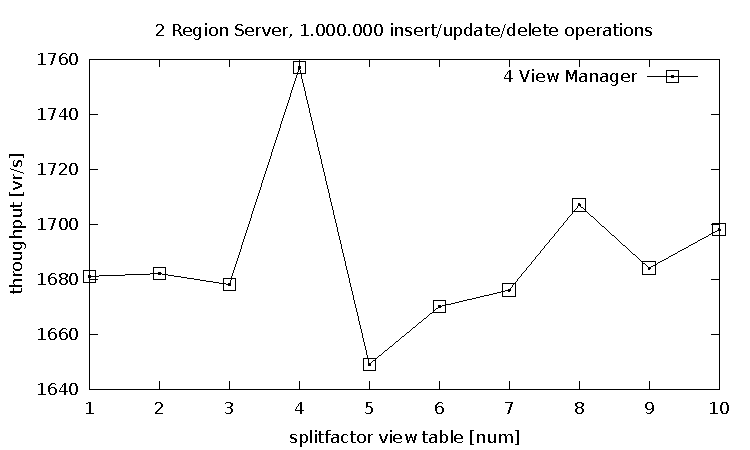
\includegraphics[width=\textwidth]{ViewTableSplit2}
    		\caption{Results Experiment 6b}
    		\label{fig:viewtablesplit2}
		\end{subfigure}		
\end{figure}



Figures \ref{fig:viewtablesplit} and \ref{fig:viewtablesplit2} present the results of the experiments 6a and 6b. On the x-axis, the number of View Managers is shown. Every point denotes a cycle of the experiment. On the y-axis, the average throughput of the complete View Maintenance System is depicted. We discover, that increasing the split factor, changes the throughput. However, we have only small variations up to 50 view records per second. In Figure \ref{fig:viewtablesplit}, the curve rises until it reaches a maximum at a split factor of 7 to 8 view table Regions. The split factor apparently corresponds to the amount of View Managers involved in the view processing. Splitting the view table increases the chances of parallel processing, but only if the number of Regions is about the number of View Managers used. This assumption is supported by Figure \ref{fig:viewtablesplit2}. Here, only four View Managers are used, instead of eight. Suddenly, the maxmima are located at a split factor of 4 and 8. Both points are a multiple of four.


\section{Experiment 7}
\label{sec:experiment7}


In order to recover from crashes, we let the View Managers write to a Commit Log. The Commit Log is located in the underlying HDFS structure. For that reason, the View Managers directly access the client API of HDFS. Since HBase itself is using the HDFS to write logs and table files, the Commit Log influences the overall performance. The more View Manager we start, the more operations are written to HDFS in parallel. In \ref{sec:experiment1} we used the Commit Log. For this experiment, we completely deactivate the Commit Log. We expect a slight increase in performance. 


In Figure \ref{fig:commitlog}, the results of experiment 7 are presented.  On the x-axis, the number of View Managers is shown. Every point denotes a cycle of the experiment. On the y-axis, the average throughput of the complete View Maintenance System is depicted. The throughput is measured in calculated view records per second. The results show, that the throughput of the system is approximately 500 view records per second faster without the use of the Commit Log. However, the shape of the curve remains the same. This is comprehensible, because the Commit Log adds to the reliability of the system and additional guarantees are always bound to a certain cost. In a productive enviroment, the Commit Log could also be switched off.

\newpage
\begin{figure}[h!]
    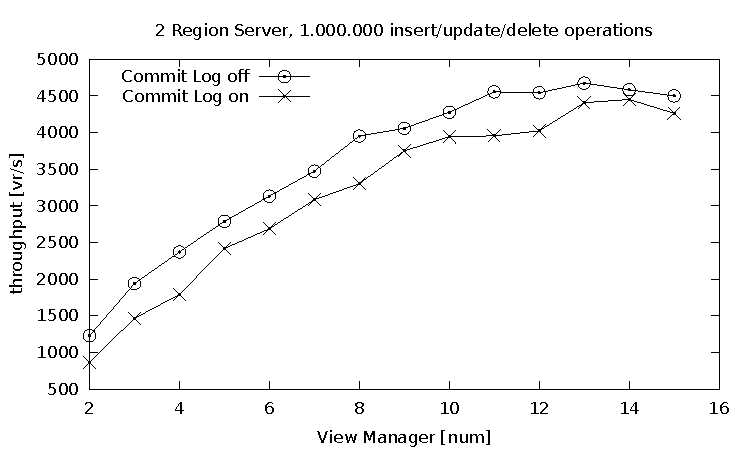
\includegraphics[width=\linewidth]{CommitLog}
    \caption{Results Experiment 7}
    \label{fig:commitlog}
\end{figure} 



\chapter{Conclusion}		
\label{chap:conclusion}

We have build a view maintenance system by using the Key-Value Store HBase. We have shown, that it is possible to calculate every type of view out of distributed data sets, efficiently. We have used the Write Ahead Log of Hbase to propagate base table updates asynchronously and establish incremental and deferred view maintenance. We have build a view maintenance architecture by extending the Region Servers of HBase and applying several patterns from the HBase architecture. We have created the View Manager, a unit of scalability, that can be assigned to Region Server dynamically and perform any update processing task. We have designed a Master component, that controls the system and that is able to react to system events by performing load balancing and recovery actions. We have discussed issues of consistency within the architecture. We have classfied the threats to consistency. We have discussed each class by analyzing examples of different view types. We have designed solutions to avert the threat scenarios. Thereby, we have used build-in features of Hbase, e.g. Test-and-Set methods, as well as established concepts of Distributed Systems, e.g. Consistent Hashing. We have established flow control within our system. We have achieved the goal of parallelising update processing and simultaneously guaranteeing consistent data within our architecture. We have developed load balancing concepts, in order to react to unequal update loads and to efficiently use the given resources. We have discussed fault tolerance and equipped the system with automatic recovery mechanisms. 
We have integrated the View Maintenance System with HBase, Zookeeper and HDFS and have described the interfaces as well as the implementation accurately.  Finally, we have evaluated System by conducting seven experiments. We have proven the scalability of the system within a certain range. We are convinced, that the architecture is able to scale linearly, even beyond the point of the measured limits. We have shown, that the View Maintenance System is able to process sum, count, min, max, selection and k-fk join views . In order to test the systems robustness, we have applied operation sets of different distribution, size and composition. We have conducted several experiments, showing the performance of the different view types. We have discovered, that performance is influenced by many factors and that we have to be careful when changing system parameters. 

	
\chapter{Future Work}	
\label{chap:futurework}

There are some points, we leave open to future work. We designed the View Managers to only support basic types of views. As a next step the View Managers could be equipped with a query language to support also nested constructions.
We have only implemented and tested the crash of a View Manager. The crash of the Region Server has been designed conceptually, but not fully implemented. The realization is more a technical challenge because the recovery has to be performed in accordance to the HBase recovery mechanisms.  However, the implementation should be manageable in reasonable time.

The versioning approach, suggested in Chapter consistency, to get rid of update interference cannot be realized with the current version of HBase. We need a method in the client API, that is not provided. The queries sent to the base table need to be evaluated with regard to the local base states at the Region Servers. Because the HBase API abstracts from the underlying architecture, there is no possibility to send requests, specifying a base table state for a given Region Server. HBase assumes, that all Region Servers are synchronized in time. Since, HBase stores enough information to answer such a query, ways have to be found to work around the probleme.

We developed the View Managers to process the view types sum, count, min, max and selection. Moreover we implemented the a special case of join view. The k-fk join view facilitates the update procedure and speeds up view maintenance to a great extent. Especially, for Key-Value Stores the general processing of join views is bound to high cost. Consider a join view, where columns are joined on non-primary keys. Then table scans have to be executed for every insert operation, that is issued. For that reason, it would be interesting to further research the different types of joins and the implication of these joins to the View Maintenance System.

Finally, the View Maintenance System should be further evaluated. We evaluated the system on a server cluster with many CPU cores and fast hard drives. The nodes of the network were build on top of a virtualisation enviroment. It would be interesting, how the View Maintenance System performs when facing the latency and hardware distribution of a typical Local Area Network.








		% ---------------------------------------------------------------------------
		%
		% Appendix
		%
		% ---------------------------------------------------------------------------
		
		\part*{Appendix}
		\addcontentsline{toc}{part}{Appendix}
		
		\appendix %---------------------------------------
		
		\chapter{Components}
%\section{Detailed Validation Results}
\label{chapter:Components}

\section{VM Master}


\textbf{Interface}

\begin{enumerate}
	\item Ingoing
	\begin{itemize}
		\item $viewManagerAdded$
		\item $viewManagerAssigned$
		\item $viewManagerRemoved$
		\item $viewManagerWithdrawn$
		\item $viewManagerReassigned$
		\item $regionServerAdded$
		\item $regionServerRemoved$
		\item $callLastCommitedUpdate$
	\end{itemize}
	\item Outgoing
	\begin{itemize}
		\item $createZookeperNode$
		\item $assignViewManager$
		\item $reassignViewManager$
		\item $withdrawViewManager$
		\item $removeViewManager$
		\item $replayWriteAheadLog$

	\end{itemize}
\end{enumerate}


\textbf{Subcomponents}

\begin{enumerate}
	\item $VM\:Master\:Controller$
	\item $Event\:Processor$
	\item $Load\:Balancer$
	\item $Recover\:Manager$
	\item $Component\:Controller$
\end{enumerate}
\newpage
\begin{figure}[h!] 
  \centering
    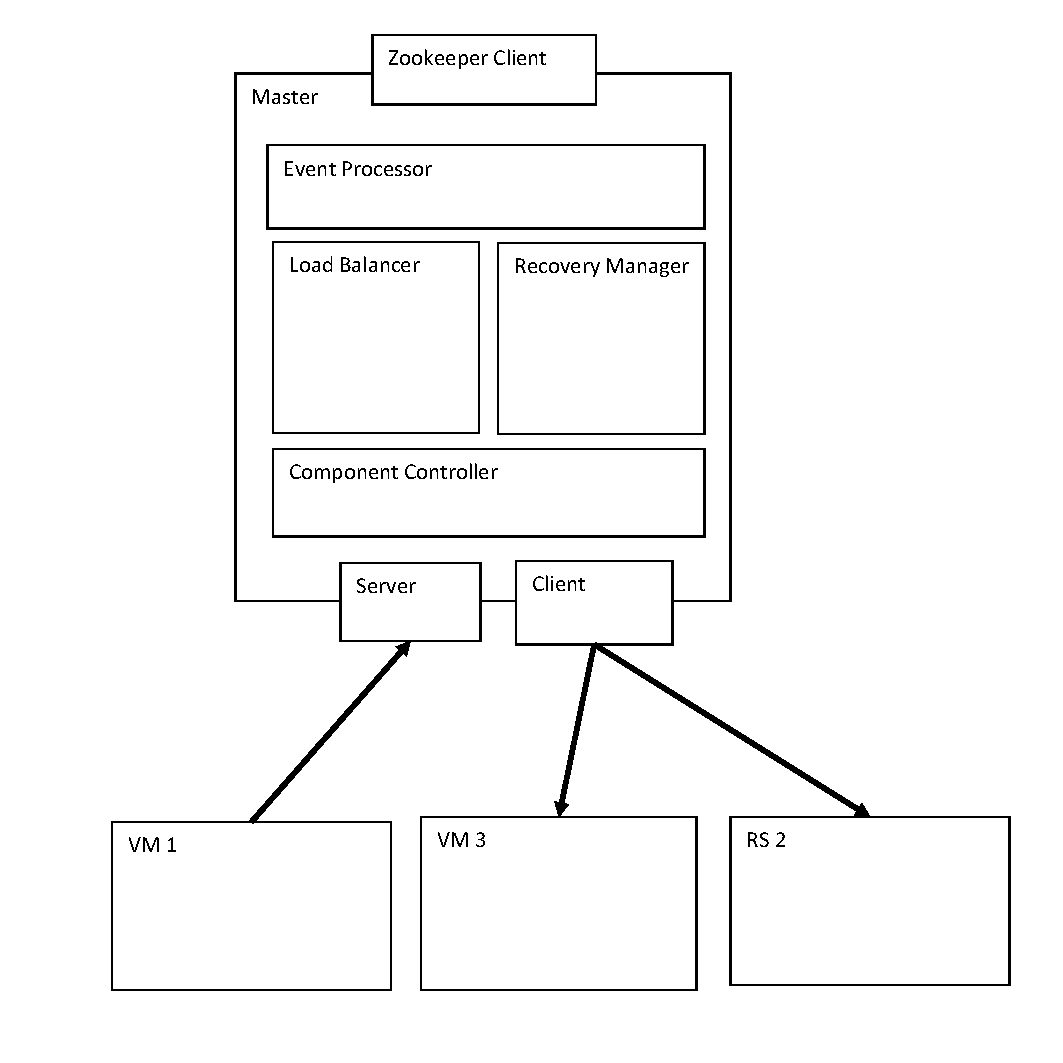
\includegraphics[scale=0.8]{figures/Master}
    \caption{Master}
    \label{fig:master}
\end{figure}

\newpage

\section{VM Region Server}

\textbf{Interface}

\begin{enumerate}
	\item Ingoing
	\begin{itemize}
		\item $put, get, delete$
		\item $assignViewManager$
		\item $withdrawViewManager$
		\item $replayWriteAheadLog$
		\item $statusReportViewManager$
	\end{itemize}
	\item Outgoing
	\begin{itemize}
		\item $createZookeeperNode$
		\item $sendUpdate$
		\item $sendStatusReport$
	\end{itemize}
\end{enumerate}


\textbf{Subcomponents}

\begin{enumerate}
	\item $HBase\:Region\:Server$
	\item $RS\:Controller$
	\item $Write\:Ahead\:Log$
	\item $WAL\:Reader$
	\item $Update\:Assigner$
	\item $Update\:Distributor$
\end{enumerate}

\newpage
\begin{figure}[h!]
  
  \centering
    \includegraphics[scale=0.8]{figures/RegionServer}
    \caption{Region Server}
    \label{fig:regionserverAppendix}
\end{figure}
\newpage

\section{View Manager}



\textbf{Interface}

\begin{enumerate}
	\item Ingoing
	\begin{itemize}
		\item $receiveUpdate$
		\item $assignViewManager$
		\item $withdrawViewManager$
		\item $reassignViewManager$
		\item $removeViewManager$
		\item $callLastCommitedUpdate$
	\end{itemize}
	\item Outgoing
	\begin{itemize}
		\item $createZookeeperNode$
		\item $shutdownViewManager$
		\item $assignViewManager$
		\item $withdrawViewManager$
		\item $getViewDefinitions$
		\item $sendStatusReport$

	\end{itemize}
\end{enumerate}

\textbf{Subcomponents}

\begin{enumerate}
	\item $VM\:Controller$
	\item $Pre-Processor$
	\item $Processor$
	\item $Commit\:Log$
\end{enumerate}

\newpage

\begin{figure}[h!]
  
  \centering
    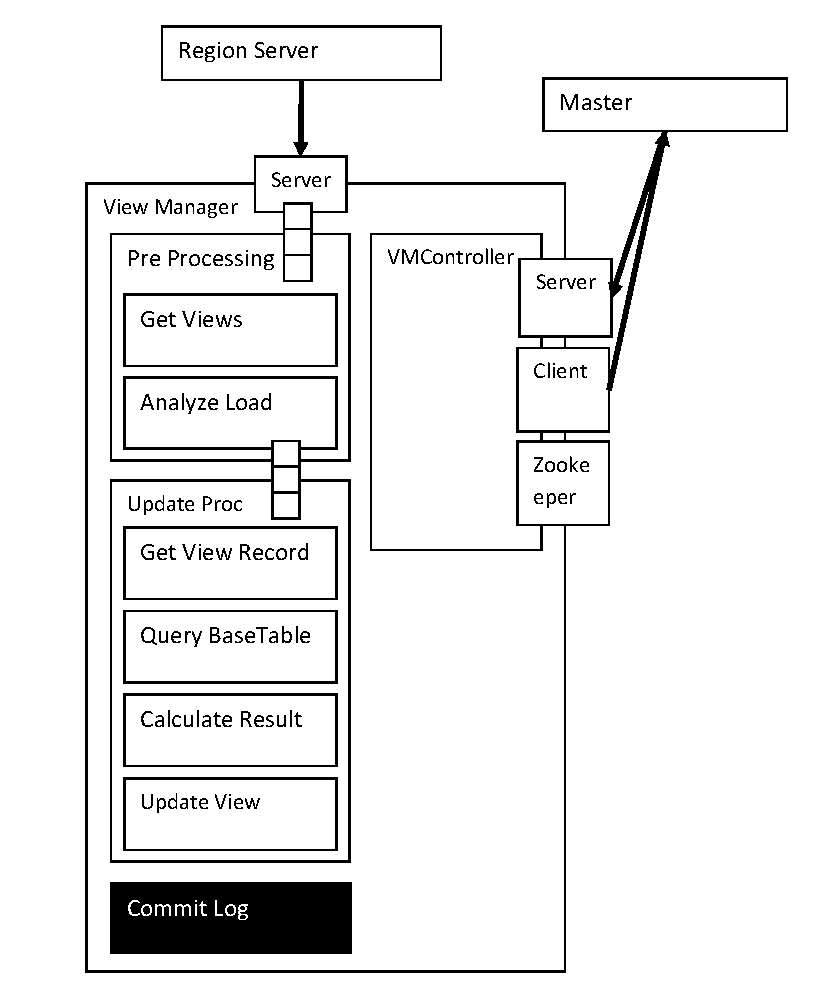
\includegraphics[width=\linewidth]{figures/ViewManager}
    \caption{View Manager}
    \label{fig:viewmanager}
\end{figure}
\newpage



\chapter{System Operations}
\label{chapter:Sytem Operations}


\section{Add View Manager}
\begin{figure}[h!]
  \centering
    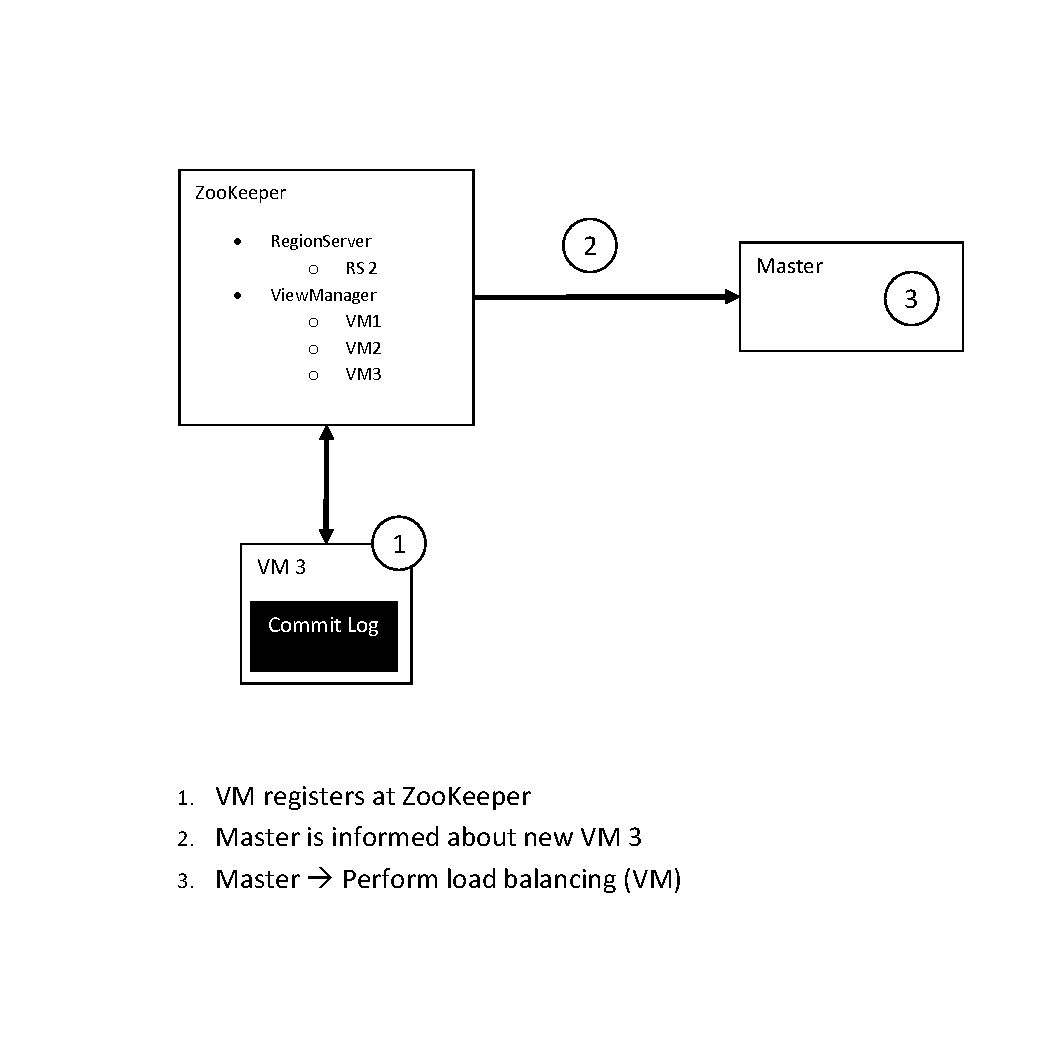
\includegraphics[scale=0.8]{figures/SO_AddViewManager}
    \caption{Add View Manager}
    \label{fig:addviewmanager}
\end{figure}
\newpage

\section{Assign View Manager}
\begin{figure}[h!]
  \centering
    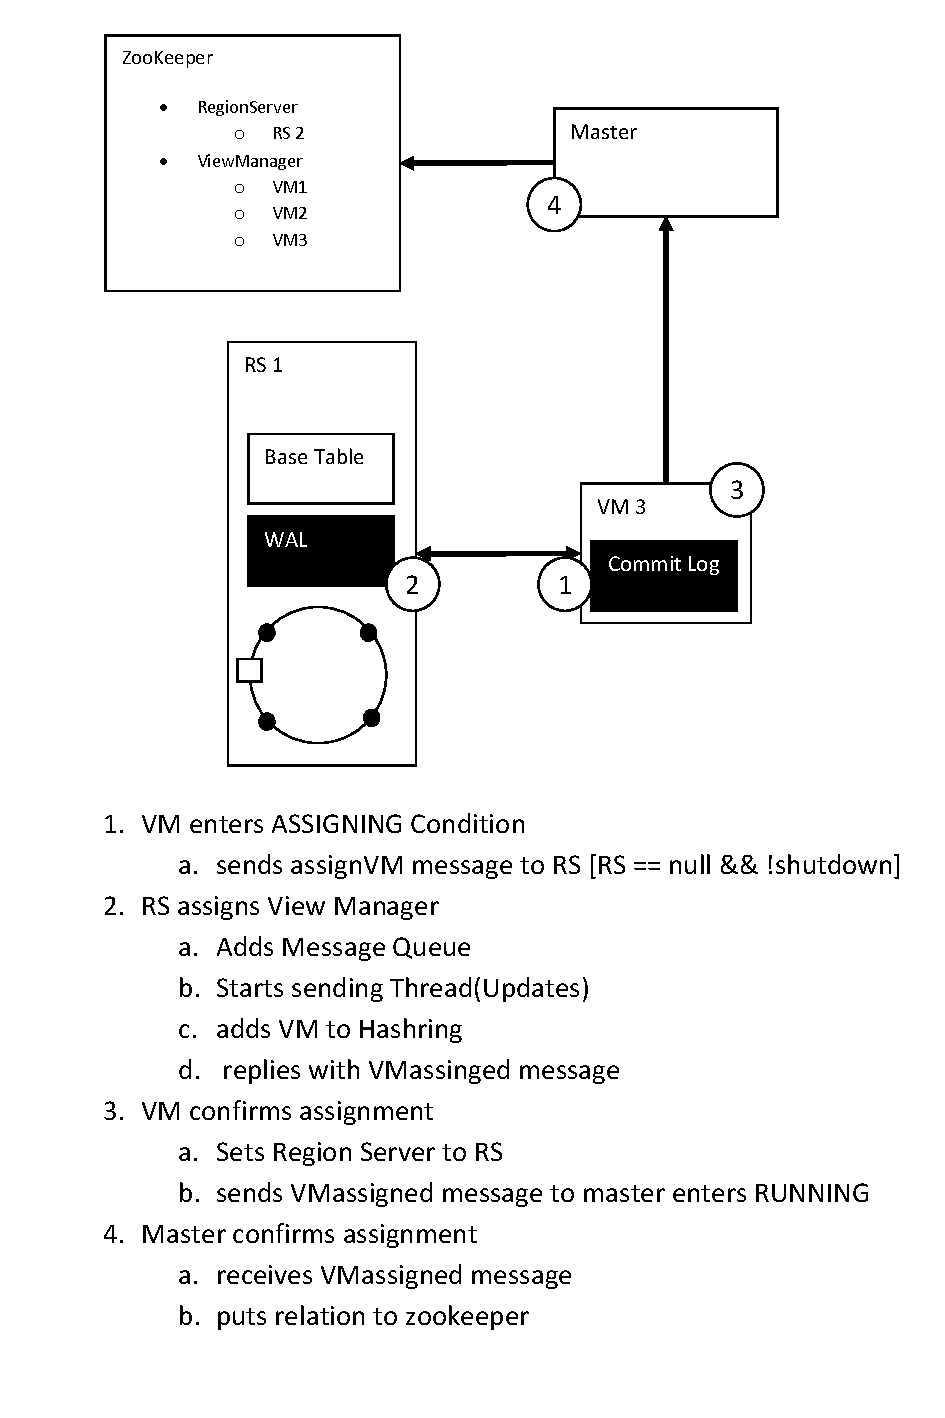
\includegraphics[scale=0.8]{figures/SO_AssignViewManager}
     \caption{Assign View Manager}
    \label{fig:assignviewmanager}
\end{figure}
\newpage

\section{Withdraw View Manager}
\begin{figure}[h!]
  \centering
    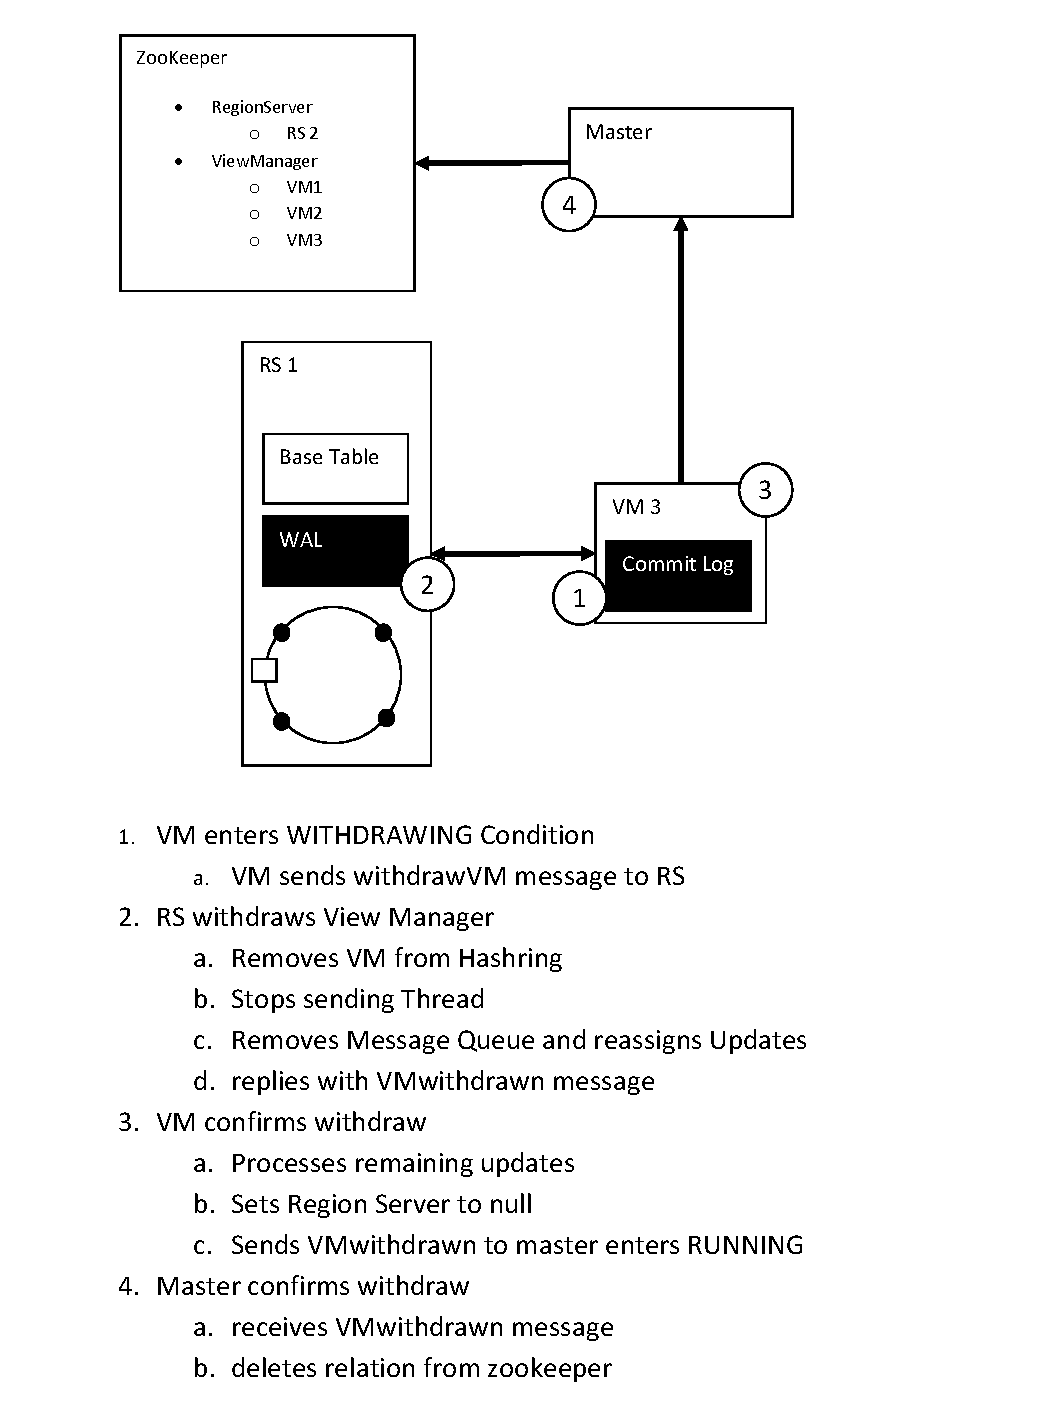
\includegraphics[scale=0.8]{figures/SO_WithdrawViewManager}
     \caption{Withdraw View Manager}
    \label{fig:withdrawviewmanager}
\end{figure}
\newpage
\section{Reassign View Manager}
\begin{figure}[h!]
  \centering
    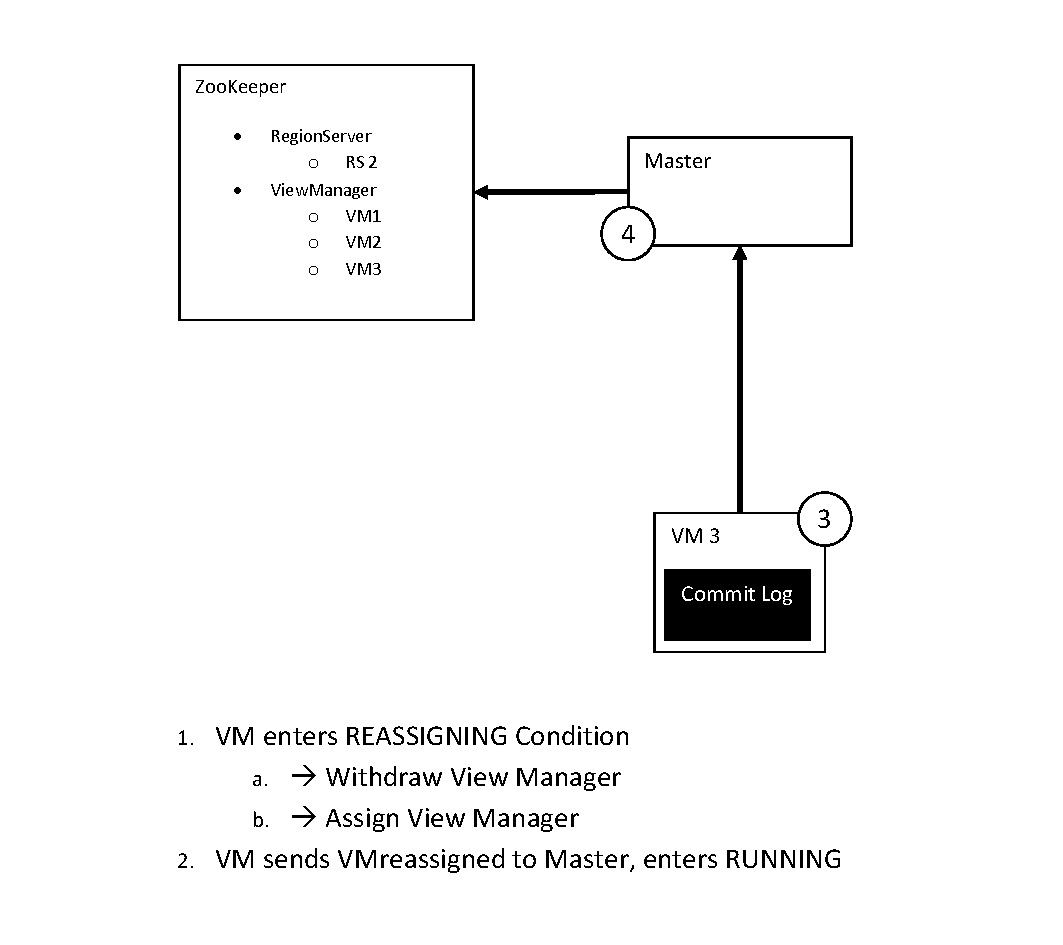
\includegraphics[scale=0.8]{figures/SO_ReassignViewManager}
     \caption{Reassign View Manager}
    \label{fig:reassignviewmanager}
\end{figure}

\newpage

\section{View Manager Crash}
\begin{figure}[h!]
  \centering
    \includegraphics[scale=0.8]{figures/SO_ViewManagerCrash}
     \caption{View Manager Crash}
    \label{fig:so_viewmanagercrash}
\end{figure}
\newpage

\section{Add Region Server}
\begin{figure}[h!]
  \centering
    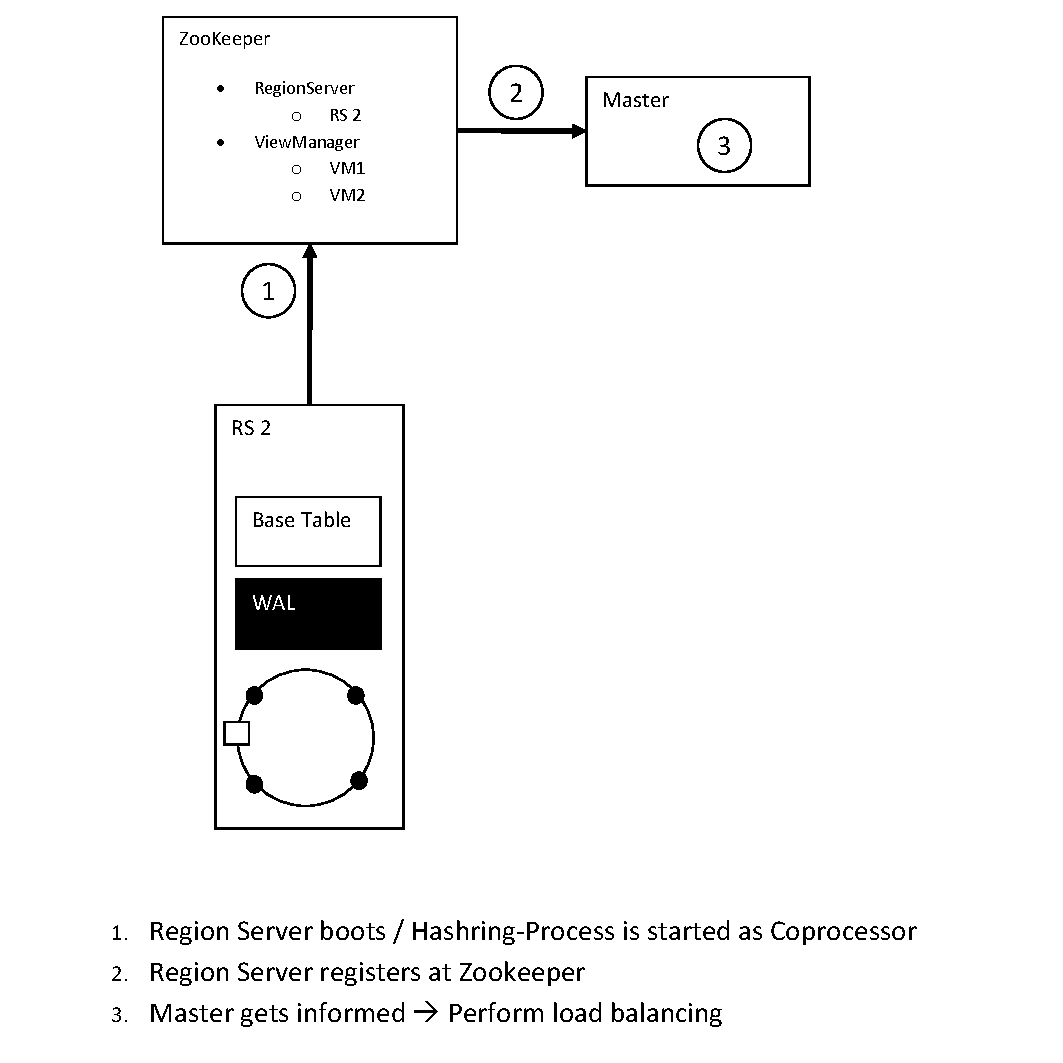
\includegraphics[scale=0.8]{figures/SO_AddRegionServer}
     \caption{Add Region Server}
    \label{fig:addregionserver}
\end{figure}
\newpage

\section{Region Server Crash}
\begin{figure}[h!]
  \centering
    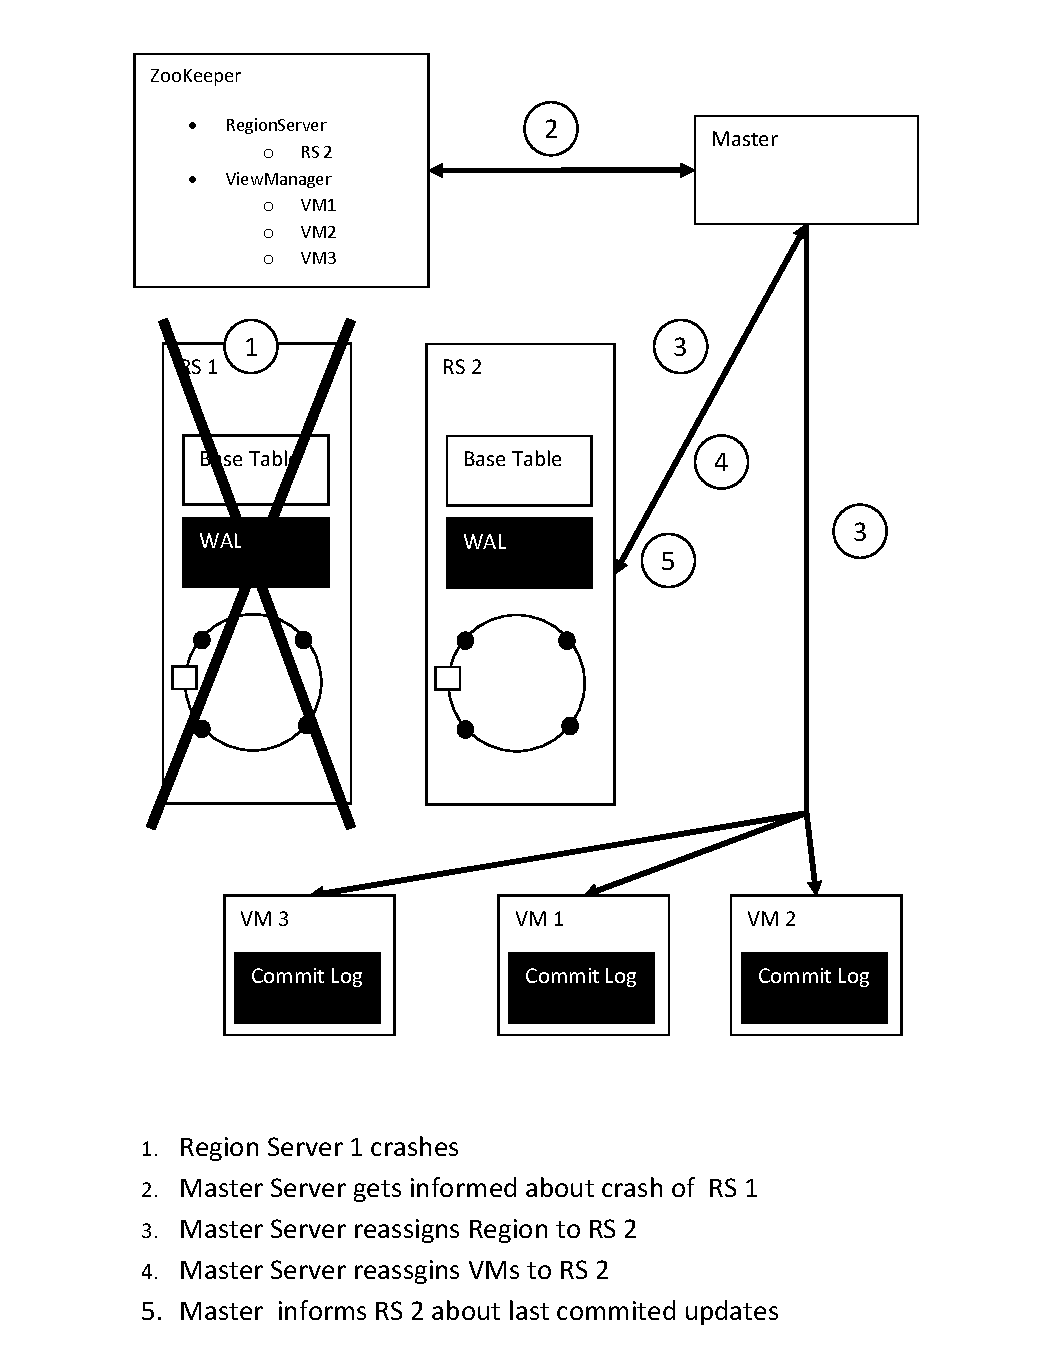
\includegraphics[scale=0.8]{figures/SO_RegionServerCrash}
     \caption{Region Server Crash}
    \label{fig:regionservercrash}
\end{figure}
\newpage

\section{Update Processing}
\begin{figure}[h!]
  
  \centering
    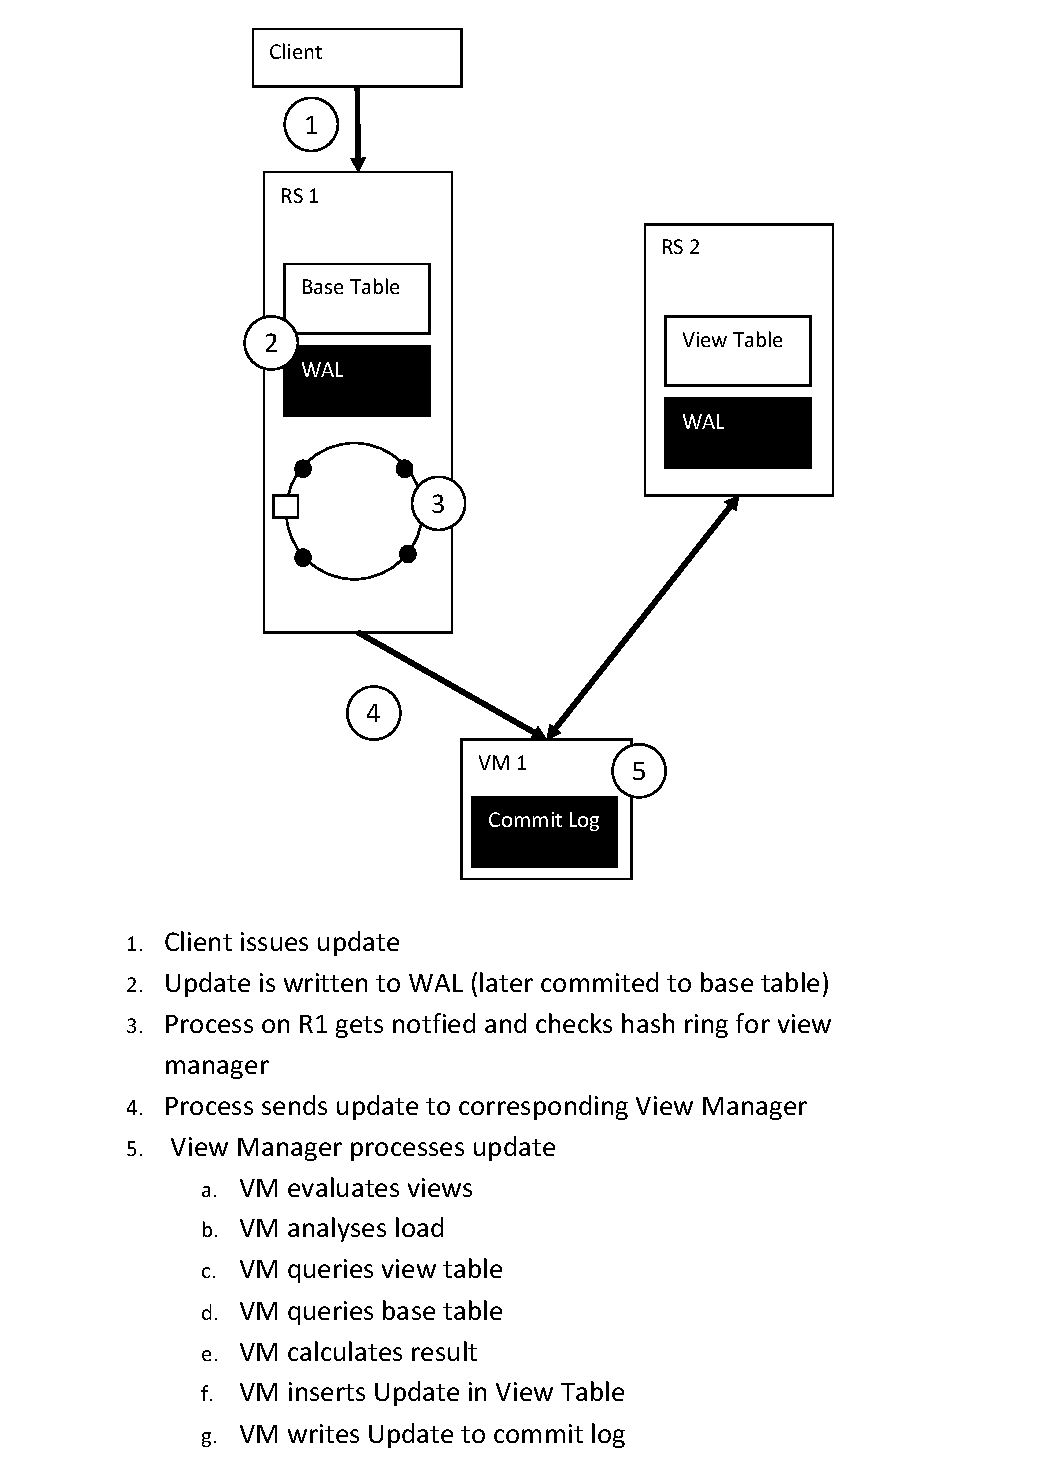
\includegraphics[scale=0.7]{figures/SO_UpdateProcessing}
    \caption{Update Path}
    \label{fig:updatepath}
\end{figure}

\newpage
\section{Status Reports}
\begin{figure}[h!]
  
  \centering
    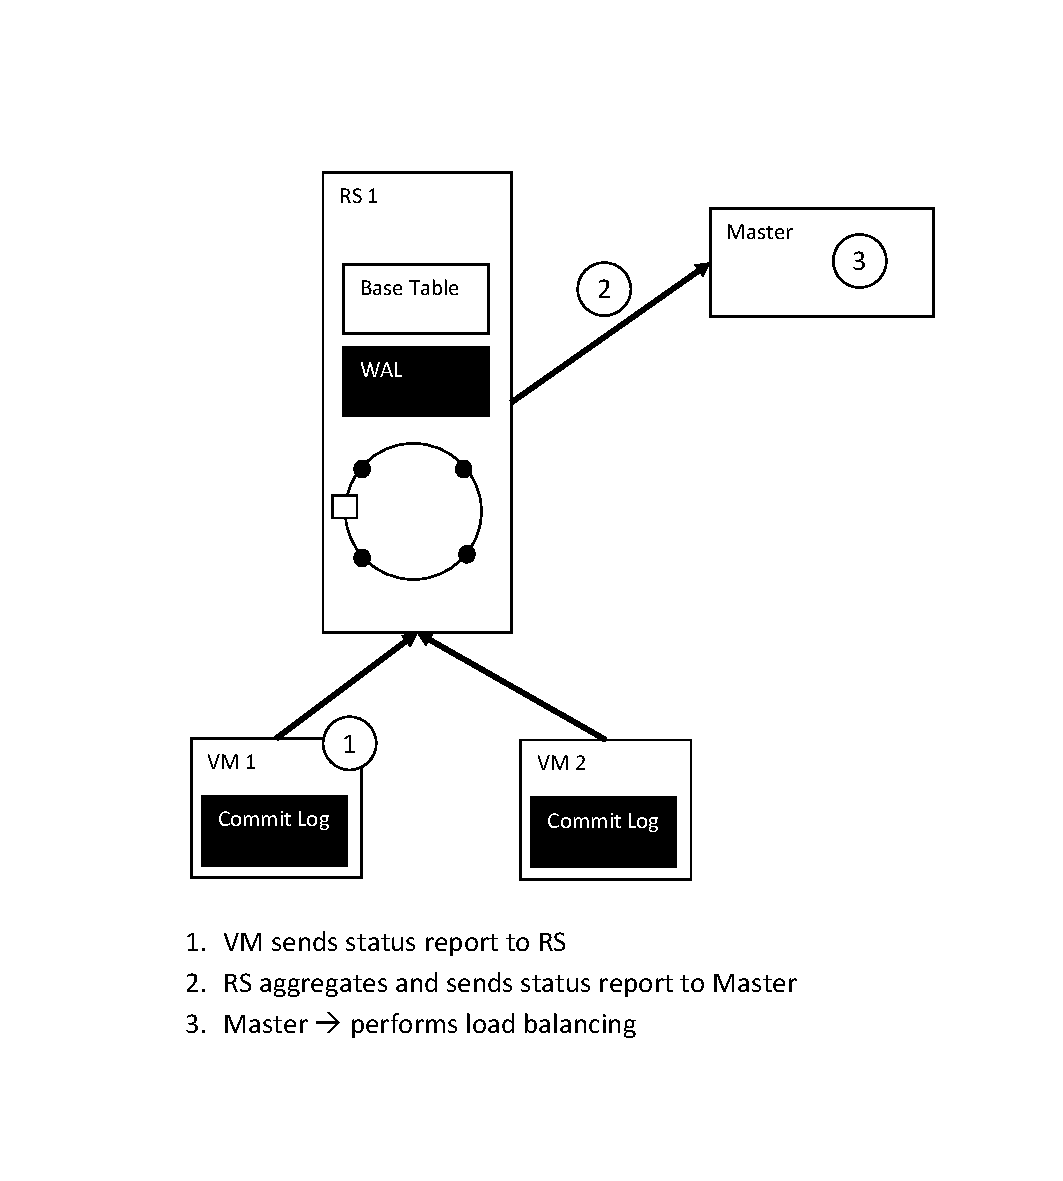
\includegraphics[width=\linewidth]{figures/SO_StatusReports}
    \caption{Status Reports}
    \label{fig:statusreports}
\end{figure}

\chapter{View Consistency}
\label{chapter:viewconsistencyappendix}


\section{Challenges to consistency}
\begin{figure}[h!]
  \centering
    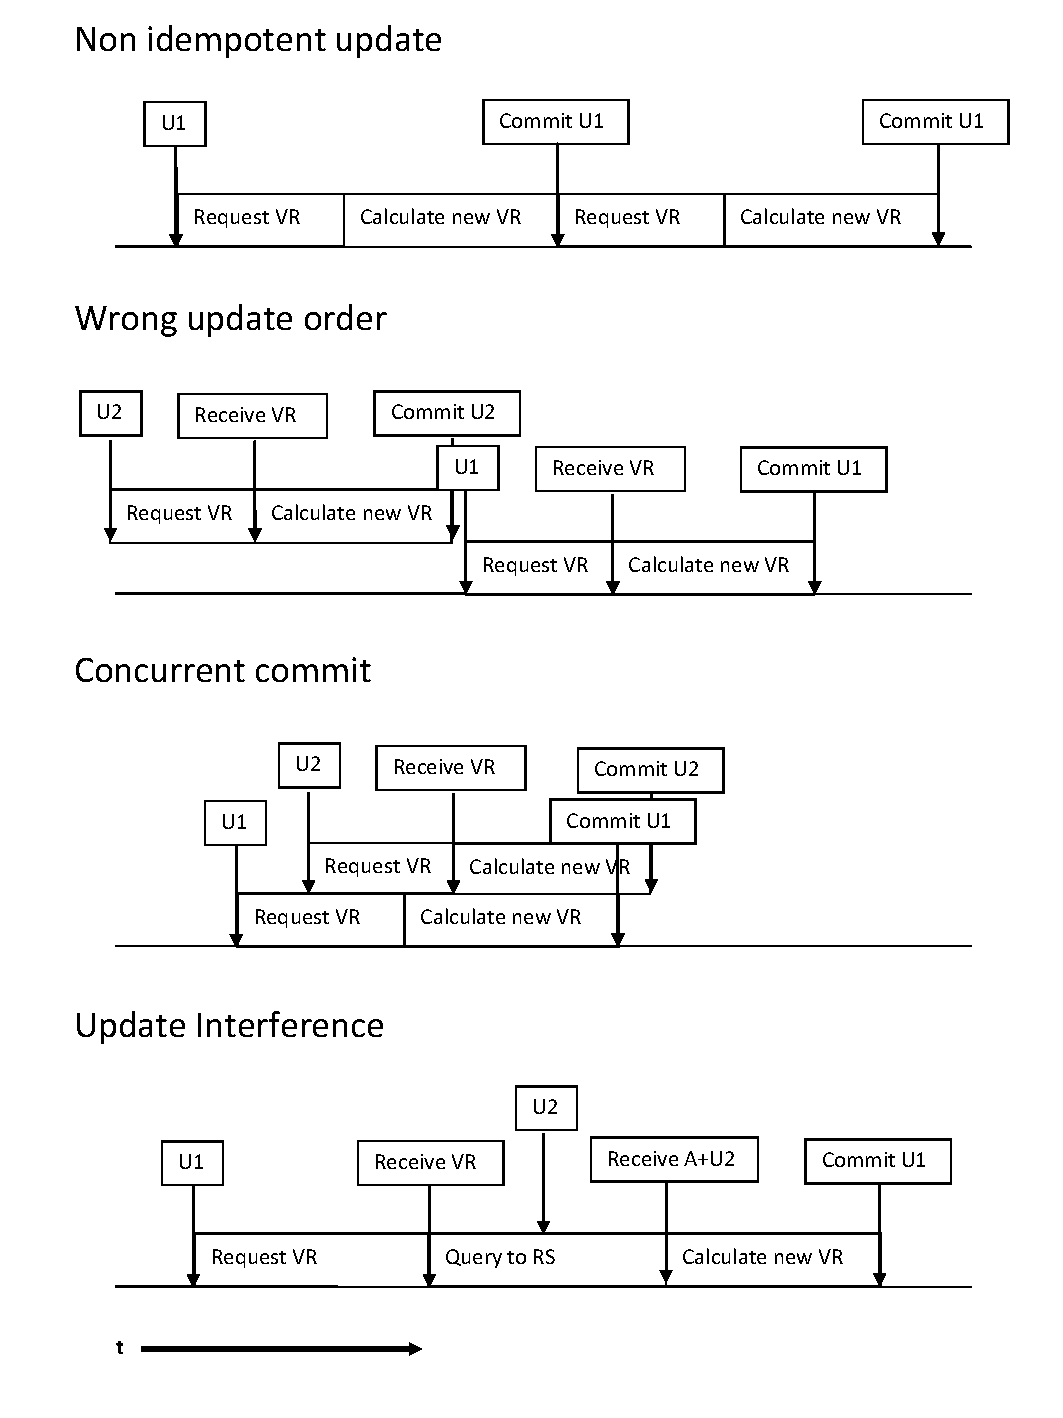
\includegraphics[scale=0.6]{figures/CO_ConsistencyProblems}
     \caption{Consistency threats}
    \label{fig:co_consistencyproblems}
\end{figure}
\newpage

\subsection{Non idempotent view updates}
\begin{figure}[h!]
  \centering
    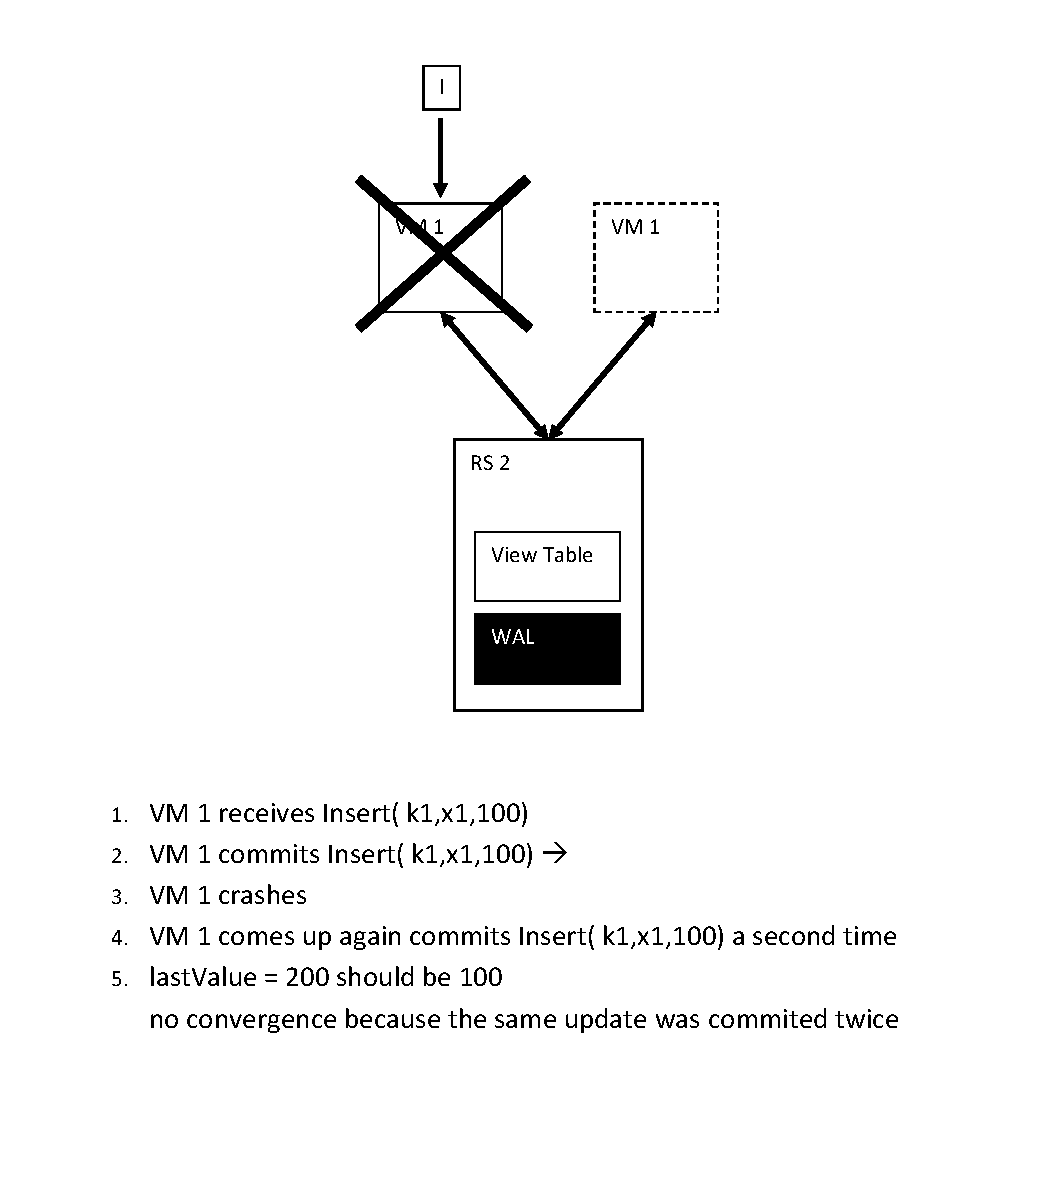
\includegraphics[scale=0.8]{figures/CO_NonIdempotentViewUpdates}
     \caption{Non idempotent view update}
    \label{fig:co_nonidempotentviewupdates}
\end{figure}

\newpage

\subsection{Wrong update order}
\begin{figure}[h!]
  \centering
    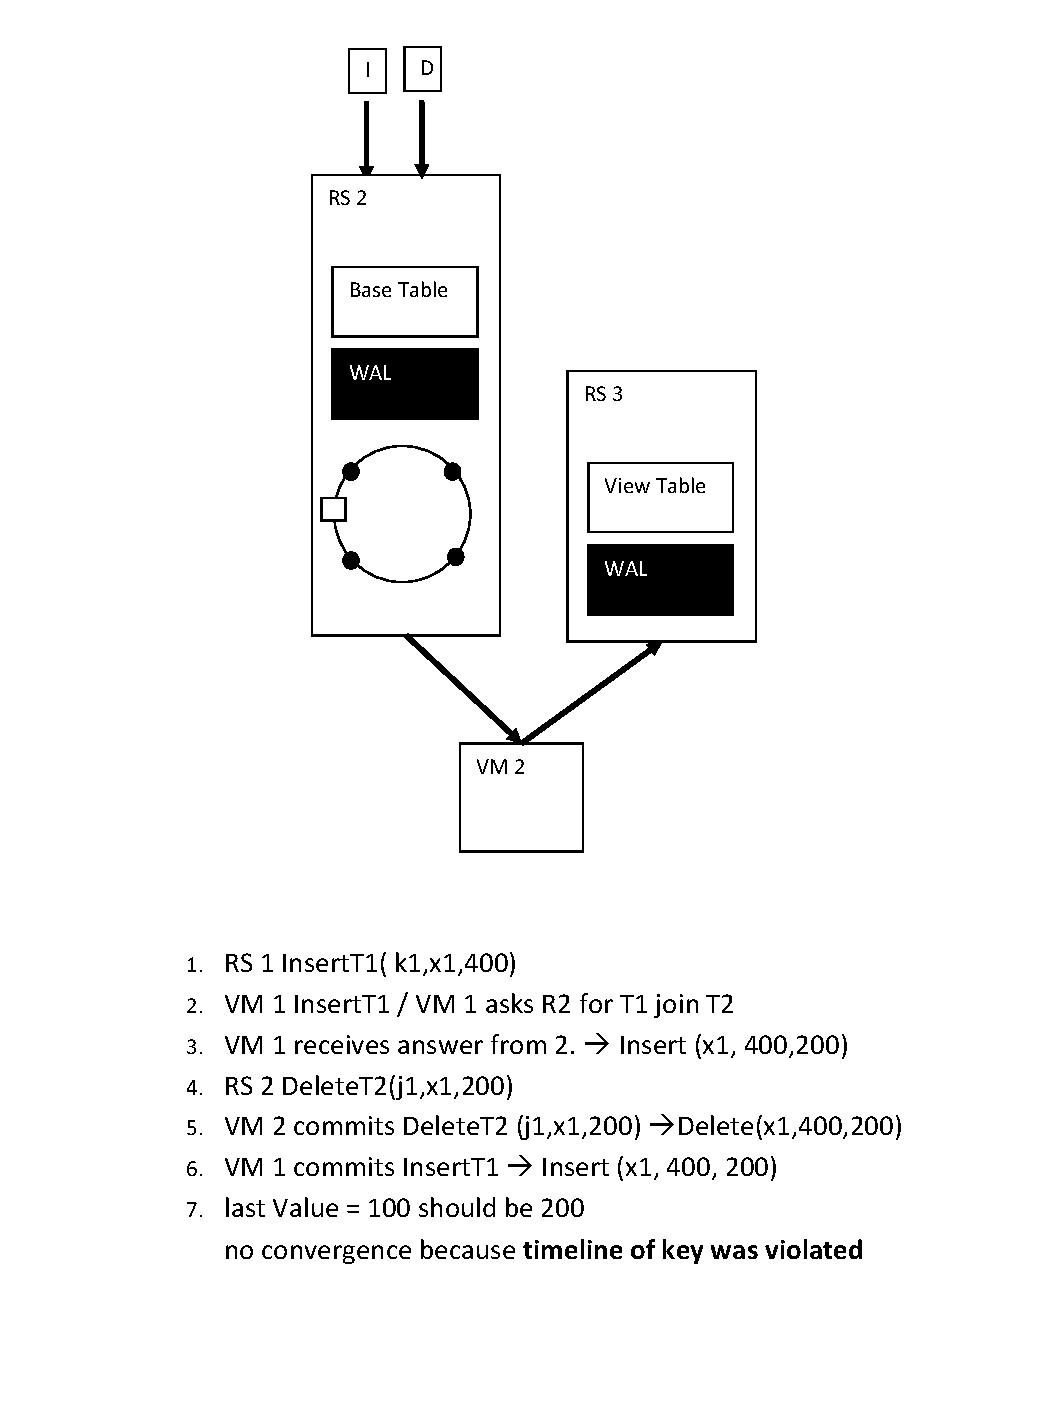
\includegraphics[scale=0.8]{figures/CO_WrongUpdateOrderJoin}
     \caption{Wrong update order join}
    \label{fig:co_wrongupdateorderjoin}
\end{figure}
\newpage
\begin{figure}[h!]
  \centering
    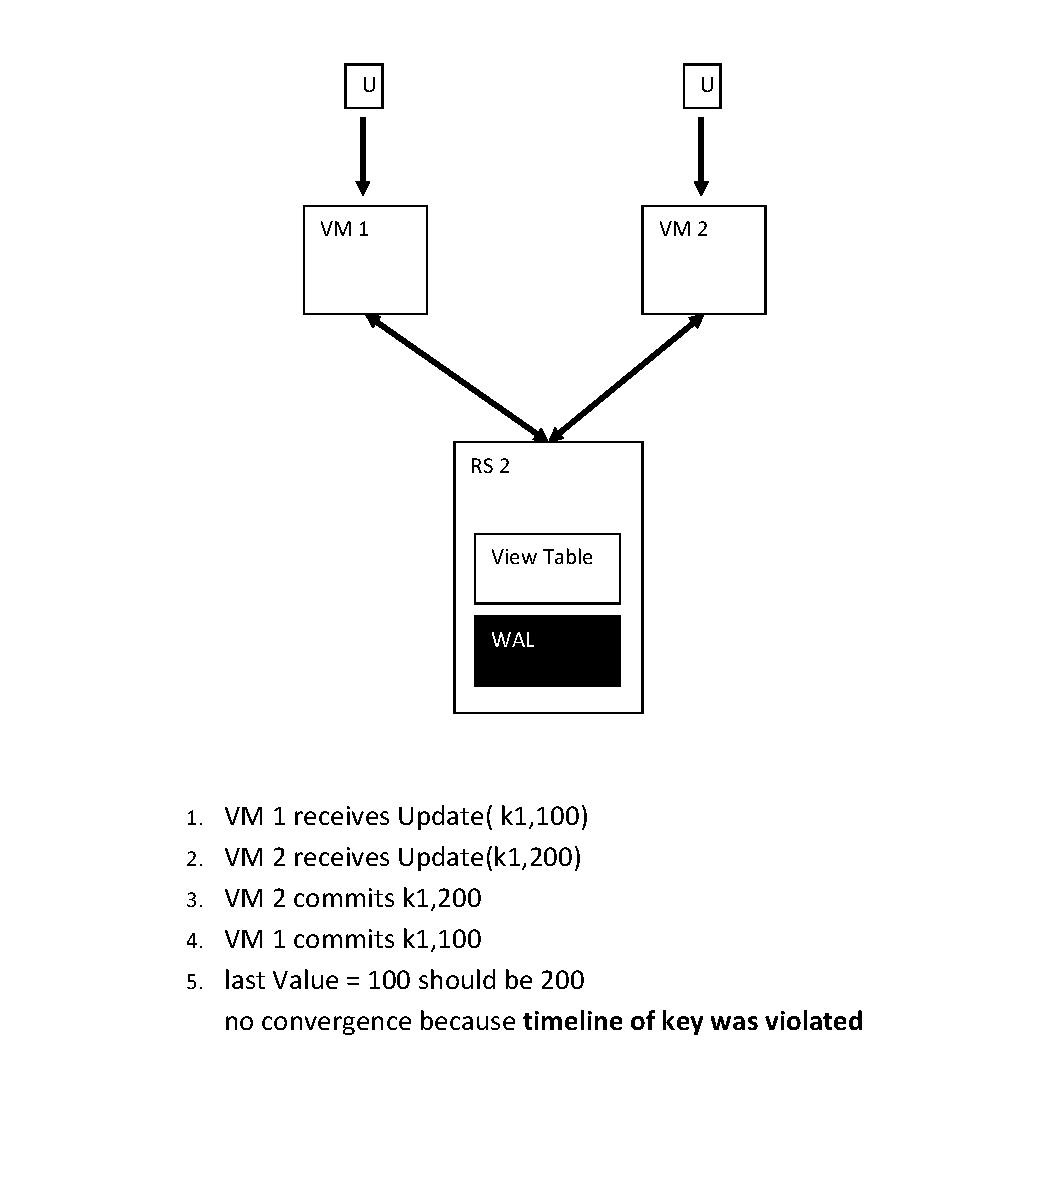
\includegraphics[scale=0.8]{figures/CO_WrongUpdateOrderSelection}
     \caption{Wrong update order Selection}
    \label{fig:co_wrongupdateorderselection}
\end{figure}
\newpage

\subsection{Concurrent commit}
\begin{figure}[h!]
  \centering
    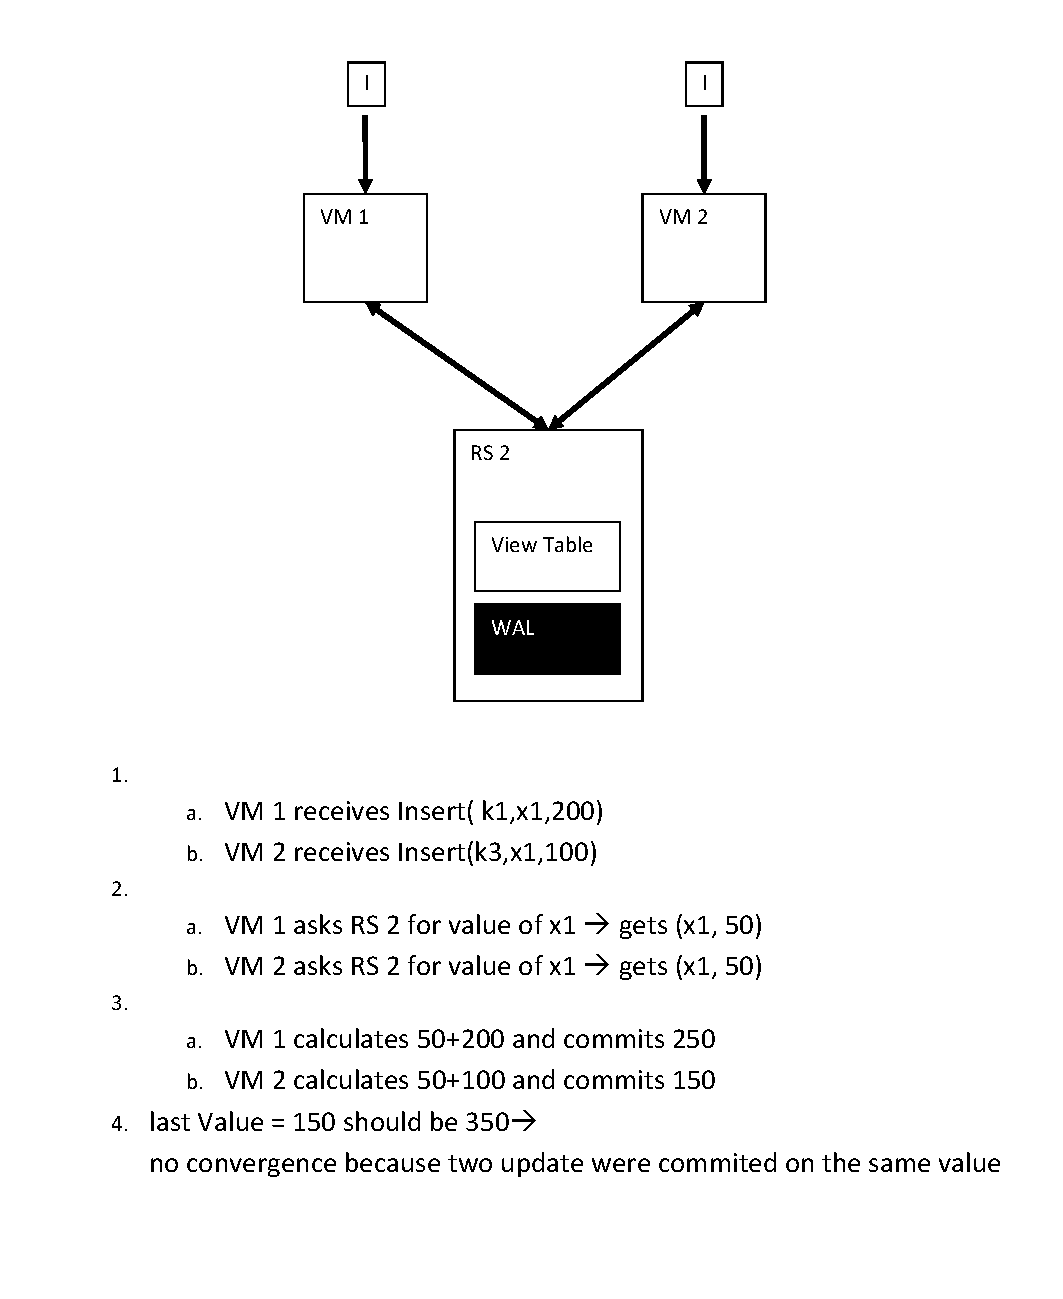
\includegraphics[scale=0.8]{figures/CO_ConcurrentCommitSum}
     \caption{Concurrent commit sum}
    \label{fig:co_concurrentcommitsum}
\end{figure}
\newpage
\begin{figure}[h!]
  \centering
    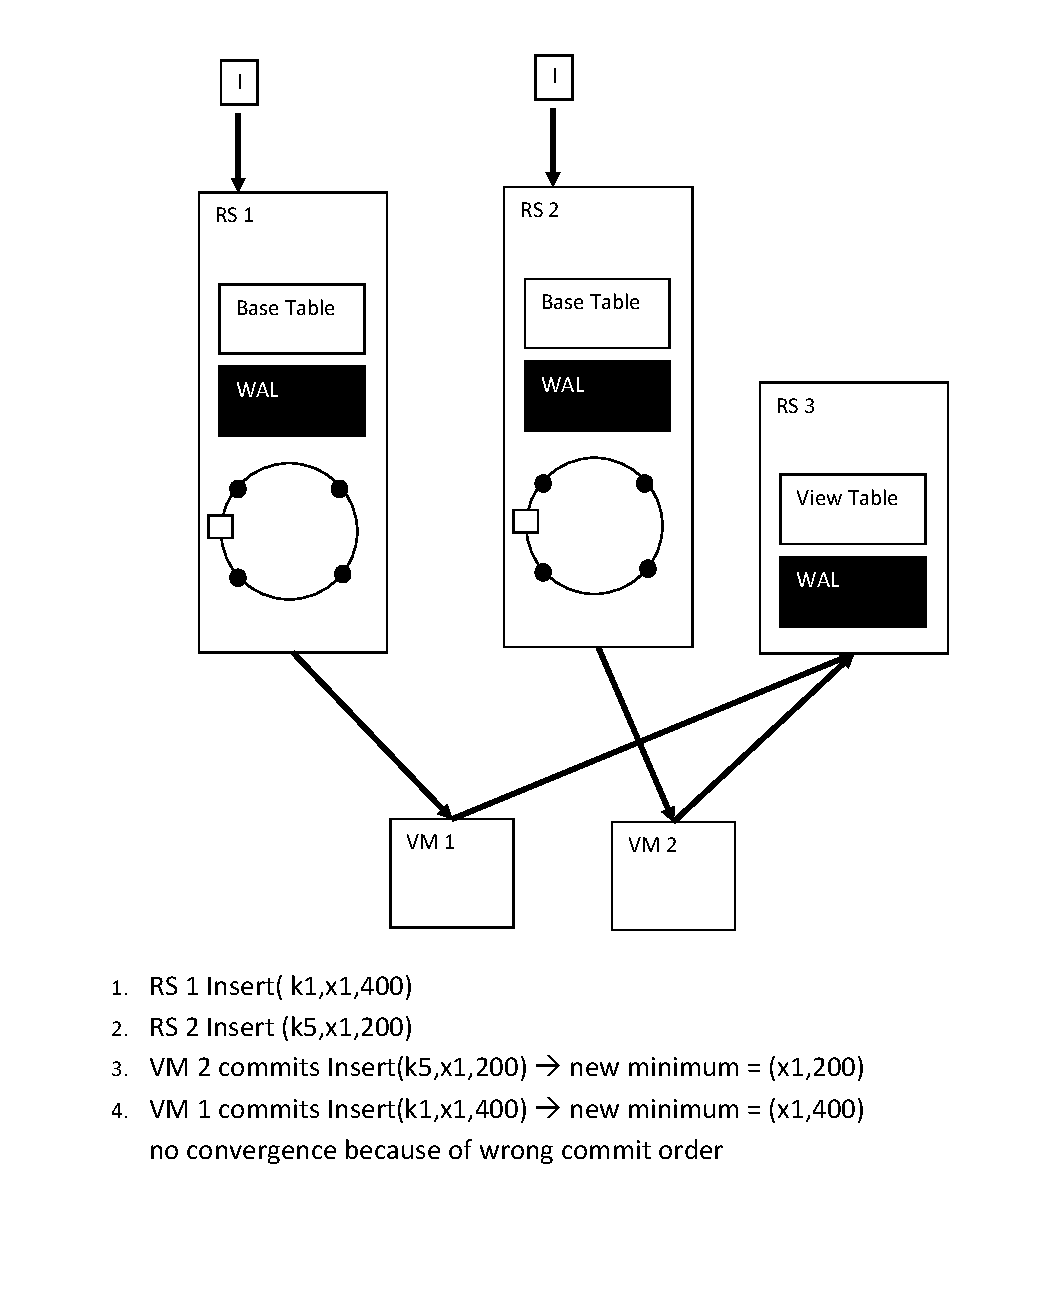
\includegraphics[scale=0.8]{figures/CO_ConcurrentCommitMin}
     \caption{Concurrent commit min}
    \label{fig:co_concurrentcommitmin}
\end{figure}
\newpage

\subsection{Update interference}
\begin{figure}[h!]
  \centering
    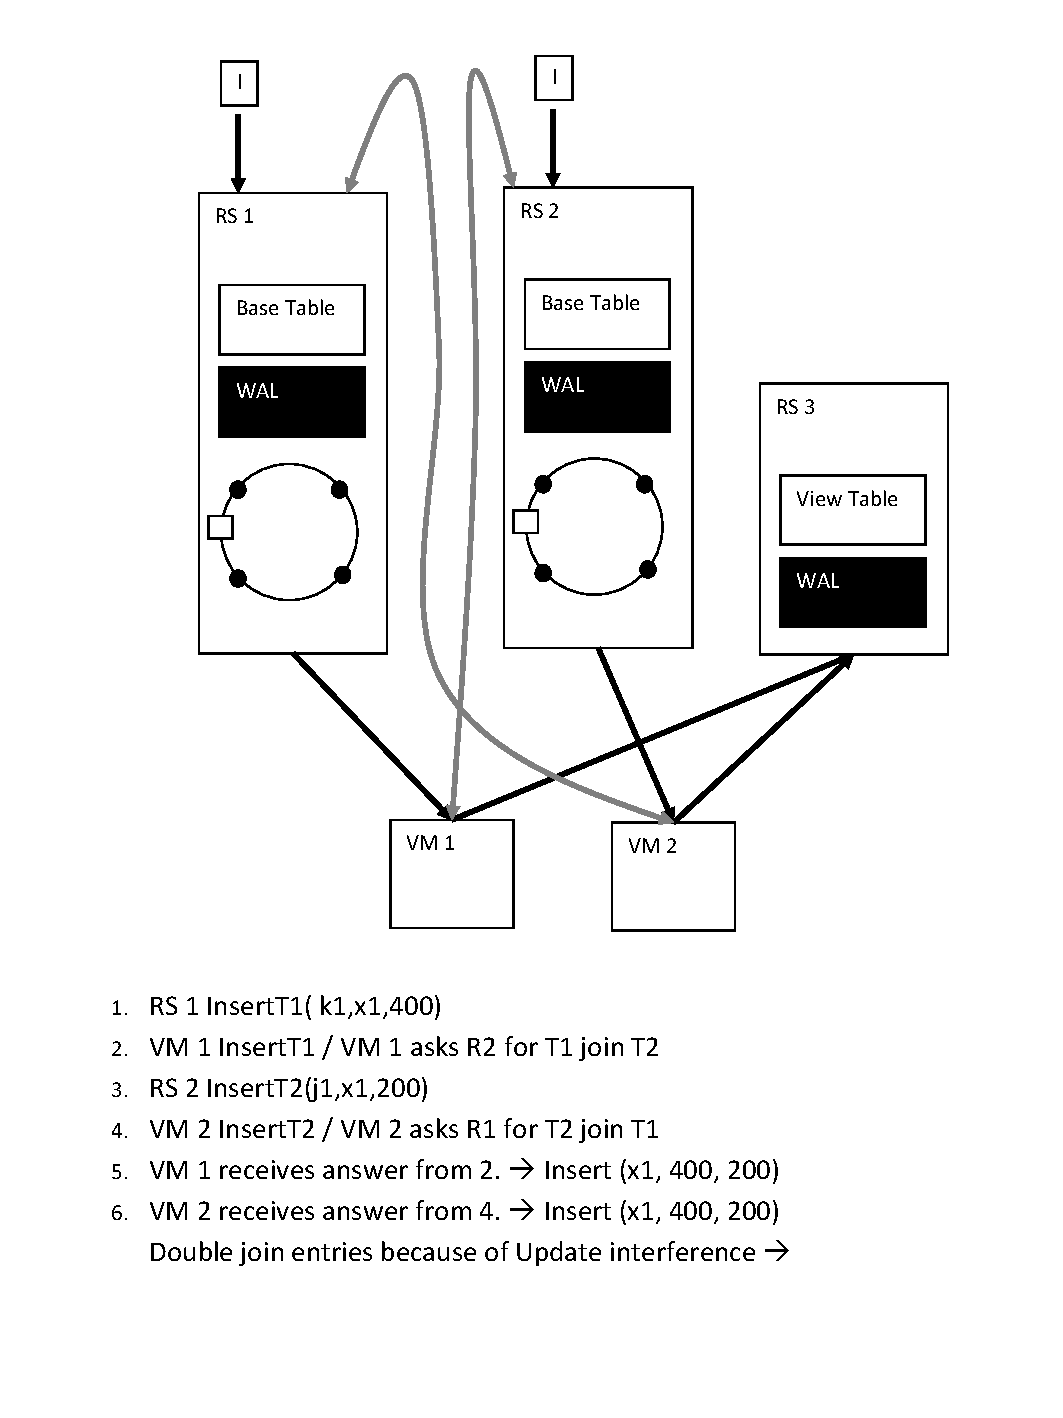
\includegraphics[scale=0.8]{figures/CO_UpdateInterferenceJoin}
     \caption{Update interference join}
    \label{fig:co_updateinterferencejoin}
\end{figure}
\newpage
\begin{figure}[h!]
  \centering
    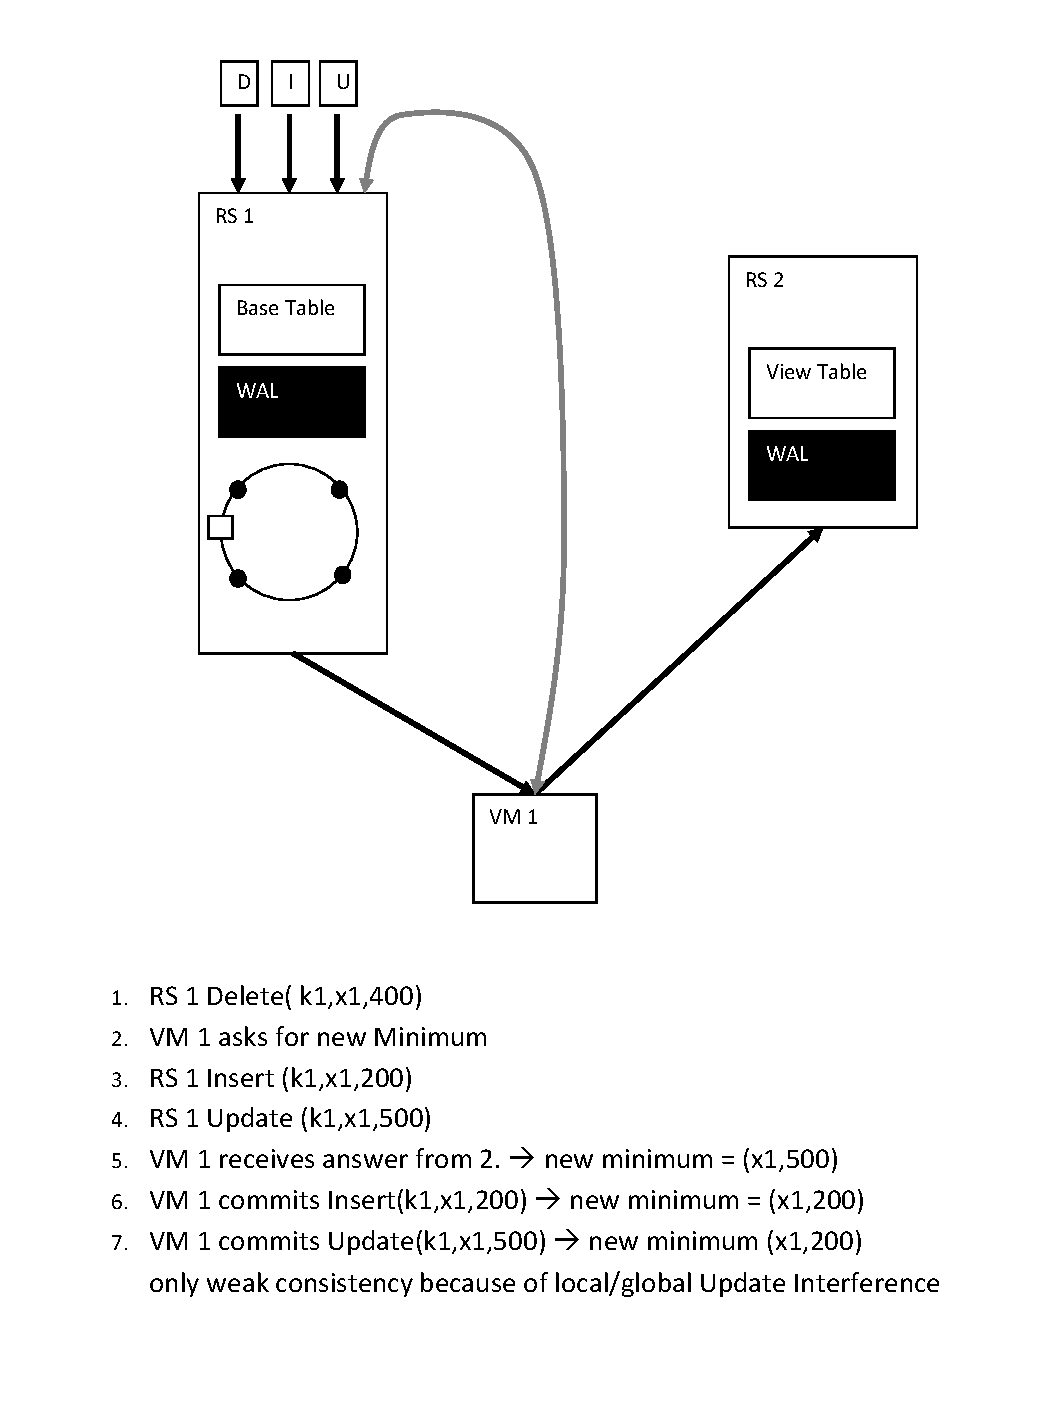
\includegraphics[scale=0.8]{figures/CO_UpdateInterferenceMin}
     \caption{Update interference min}
    \label{fig:co_updateinterferencemin}
\end{figure}
\newpage

\chapter{Load Balancing}
\label{chapter:loadbalancingappendix}


\section{Add View Manager}
\begin{figure}[h!]
  \centering
    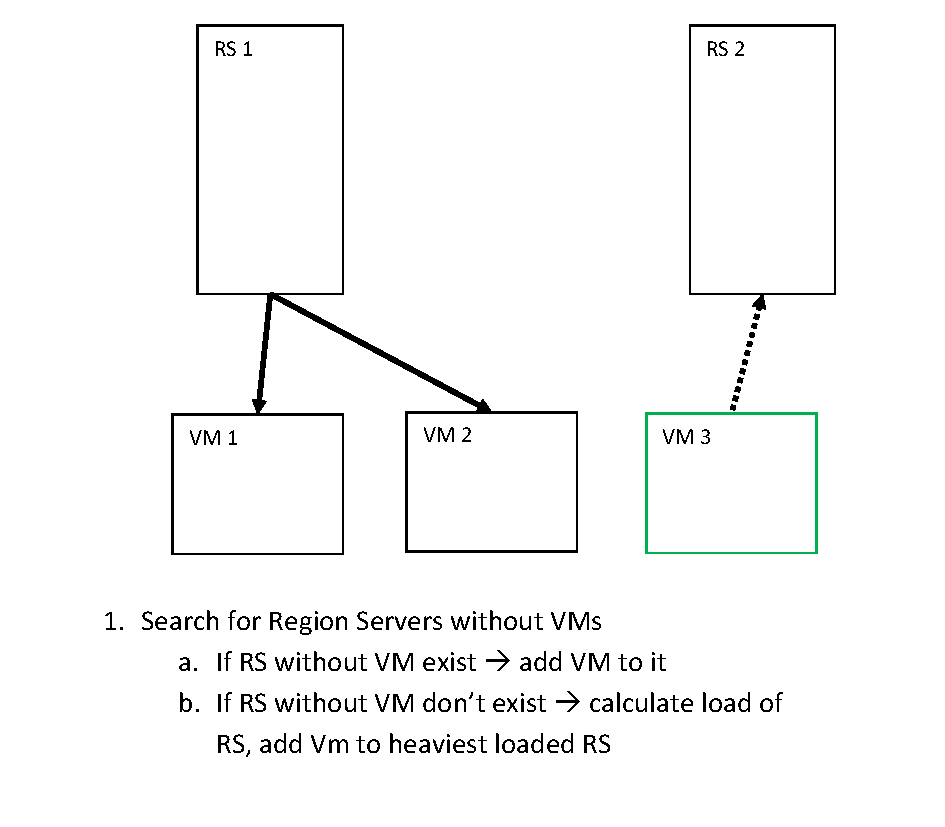
\includegraphics[scale=0.8]{figures/LB_AddViewManager}
     \caption{Add View Manager}
    \label{fig:lb_addviewmanager}
\end{figure}
\newpage

\section{Remove View Manager}
\begin{figure}[h!]
  \centering
    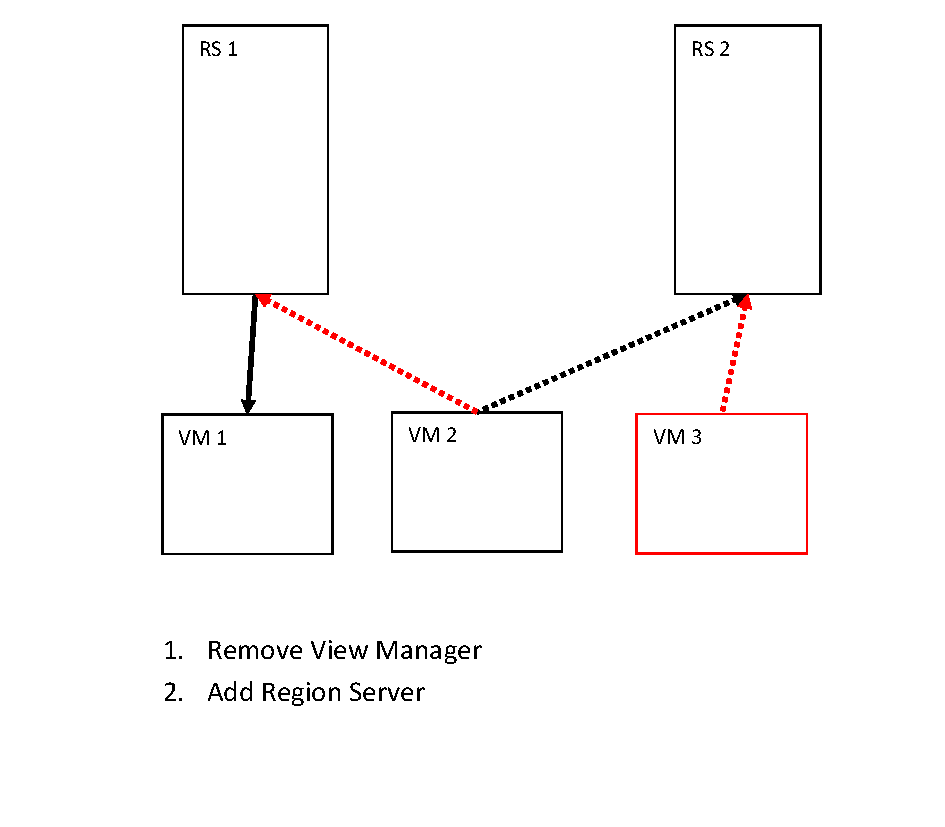
\includegraphics[scale=0.8]{figures/LB_RemoveViewManager}
     \caption{Remove View Manager}
    \label{fig:lb_removeviewmanager}
\end{figure}
\newpage

\section{Add Region Server}
\begin{figure}[h!]
  \centering
    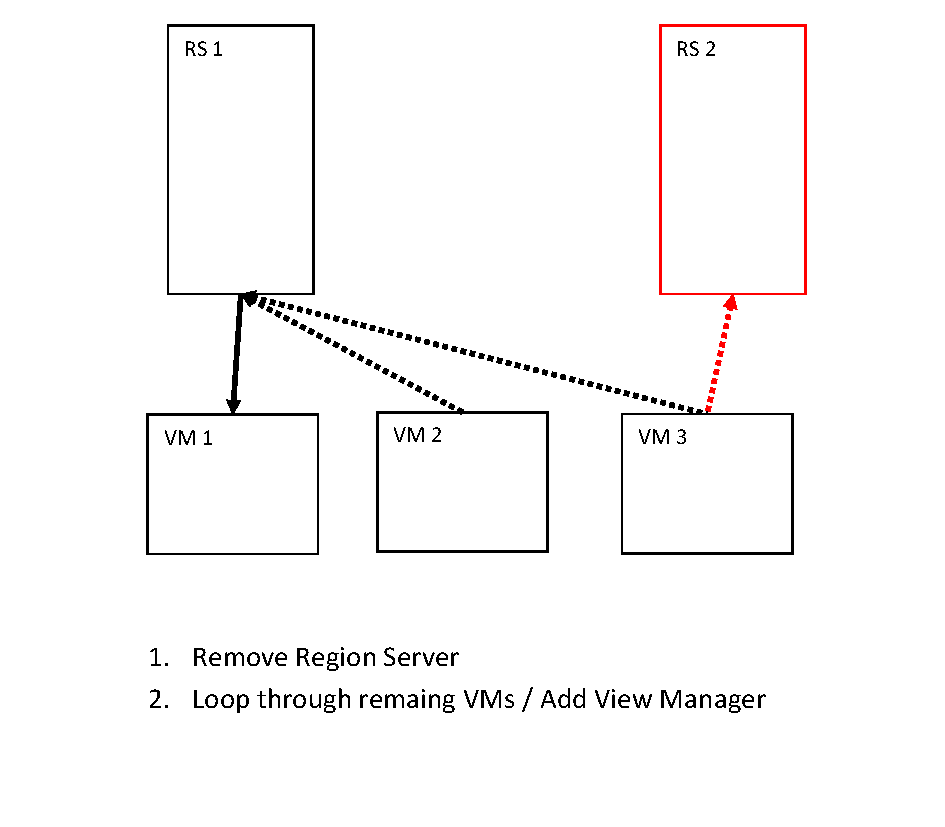
\includegraphics[scale=0.8]{figures/LB_AddRegionServer}
     \caption{Add Region Server}
    \label{fig:lb_addregionserver}
\end{figure}
\newpage

\section{Remove Region Server}
\begin{figure}[h!]
  \centering
    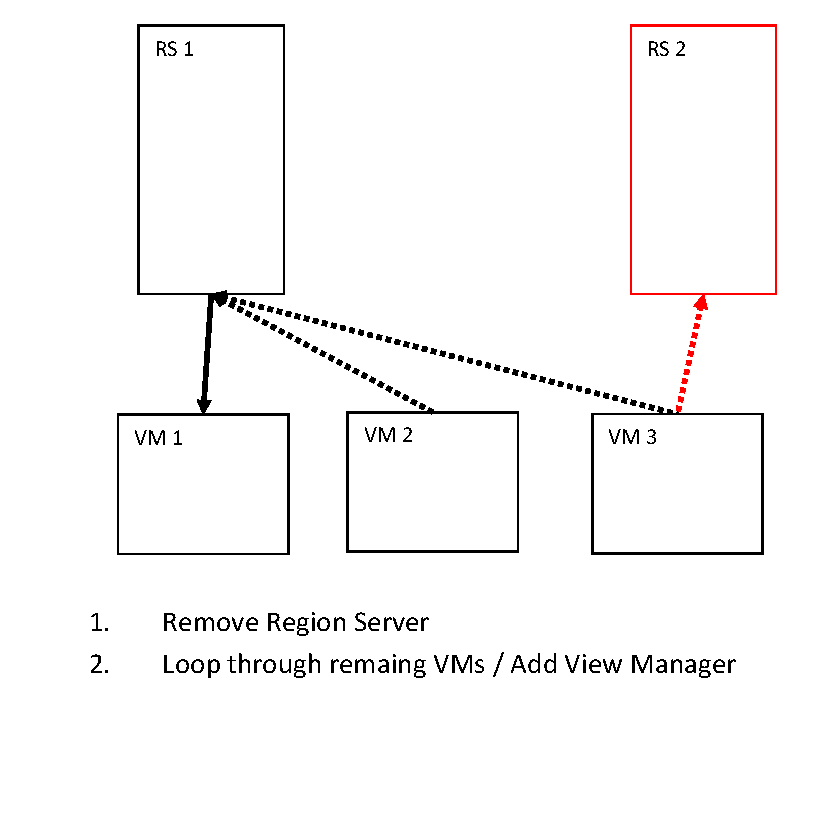
\includegraphics[scale=0.8]{figures/LB_RemoveRegionServer}
    \caption{Remove Region Server}
    \label{fig:lb_removeregionserver}
\end{figure}
\newpage




  \clearemptydoublepage
  
	\bibliography{bibliography/literature}
	
 
\end{document}

